\documentclass[a4paper,12pt,oneside]{book}
\usepackage[T1]{fontenc} % Use 8-bit encoding that has 256 glyphs
\usepackage[utf8]{inputenc}
\usepackage{fourier} % Use the Adobe Utopia font for the document - comment this line to return to the LaTeX default
\usepackage{listings} % para insertar código con formato similar al editor
\usepackage[spanish, es-tabla]{babel} % Selecciona el español para palabras introducidas automáticamente, p.ej. "septiembre" en la fecha y especifica que se use la palabra Tabla en vez de Cuadro
\usepackage{url} % ,href} %para incluir URLs e hipervínculos dentro del texto (aunque hay que instalar href)
\usepackage{graphics,graphicx, float} %para incluir imágenes y colocarlas
\usepackage[gen]{eurosym} %para incluir el símbolo del euro
\usepackage{cite} %para incluir citas del archivo <nombre>.bib
\usepackage{enumerate}
\usepackage{hyperref}
\usepackage{tabularx}
\usepackage{booktabs}
\usepackage{afterpage}
\usepackage{longtable}
\usepackage[stable]{footmisc}
\usepackage[table,xcdraw]{xcolor}
\usepackage[font=small,labelfont=bf,center]{caption}
\usepackage{subcaption}
\usepackage{placeins}
\usepackage{float}
\usepackage{adjustbox}
\usepackage{ragged2e}


% ********************************************************************
% Re-usable information
% ********************************************************************
\newcommand{\myTitle}{API para la gestión de mascotas en adopción\xspace}
\newcommand{\myTitleEn}{API for the management of animals for adoption\xspace}
\newcommand{\myDegree}{Grado en Ingeniería Informática\xspace}
\newcommand{\myName}{Manuel Ángel Rodríguez Segura\xspace}
\newcommand{\myProf}{Marcelino José Cabrera Cuervas\xspace}
\newcommand{\myFaculty}{Escuela Técnica Superior de Ingenierías Informática y de Telecomunicación\xspace}
\newcommand{\myFacultyShort}{E.T.S. de Ingenierías Informática y de Telecomunicación\xspace}
\newcommand{\myDepartment}{Departamento de Lenguajes y Sistemas Informáticos\xspace}
\newcommand{\myProject}{Trabajo Fin de Grado\xspace}
\newcommand{\myUni}{\protect{Universidad de Granada}\xspace}
\newcommand{\myLocation}{Granada\xspace}
\newcommand{\myTime}{\today\xspace}
\newcommand{\myVersion}{Version 0.1\xspace}
\newcommand{\tabitem}{~~\llap{\textbullet}~~}
\newcolumntype{L}{>{\RaggedRight\arraybackslash}X}


\hypersetup{
    colorlinks=true,	% false: boxed links; true: colored links
    linkcolor=black,	% color of internal links
    urlcolor=cyan		% color of external links
}


\renewcommand{\familydefault}{\sfdefault}
\usepackage{fancyhdr} % Custom headers and footers
\pagestyle{fancyplain} % Makes all pages in the document conform to the custom headers and footers
\fancyhf{} % clear existing header/footer entries
% HEADER
\setlength{\headheight}{13.6pt} % Customize the height of the header
\fancyhead[L]{} % Empty left header
\fancyhead[C]{} % Empty center header
\fancyhead[R]{} % Empty right header
\fancyhead[LO]{\leftmark}
\fancyhead[RE]{\rightmark}
\fancyhead[RO,LE]{\thepage}
\renewcommand{\chaptermark}[1]{\markboth{#1}{}}
\renewcommand{\sectionmark}[1]{\markright{\thesection. #1}}
% FOOOTER
\renewcommand{\footrulewidth}{0pt} % Remove footer underlines
\fancyfoot[L]{} % Empty left footer
\fancyfoot[C]{} % Empty center footer

\fancypagestyle{plain}{%
    \fancyhf{}% clear all header and footer fields
    \fancyfoot[C]{\thepage} % except the center
    \renewcommand{\headrulewidth}{0pt}%
    \renewcommand{\footrulewidth}{0pt}%
}

\fancypagestyle{coverpage}{%
    \fancyhf{}% clear all header and footer fields
    \fancyhead[L]{\myProject} % except the center
%    \renewcommand{\headrulewidth}{0pt}%
    \renewcommand{\footrulewidth}{0pt}%
}


\usepackage{titlesec, blindtext, color}
\newcommand{\hsp}{\hspace{20pt}}
\titleformat{\chapter}[hang]{\Huge\bfseries}{\thechapter\hsp{|}\hsp}{0pt}{\Huge\bfseries}
\setcounter{secnumdepth}{3} % Turn off/on section numbers (0=no numbers, 1=numbers in sections, 2=numbers in subsections ...)
\setcounter{tocdepth}{3}
%\usepackage[Lenny]{fncychap}


\newcommand{\HRule}{\rule{\linewidth}{0.5mm}}
\newcommand{\bigrule}{\titlerule[0.5mm]}


%Definimos los tipos teorema, ejemplo y definición podremos usar estos tipos
%simplemente poniendo \begin{teorema} \end{teorema} ...
\newtheorem{teorema}{Teorema}[chapter]
\newtheorem{ejemplo}{Ejemplo}[chapter]
\newtheorem{definicion}{Definición}[chapter]

\definecolor{gray97}{gray}{.97}
\definecolor{gray75}{gray}{.75}
\definecolor{gray45}{gray}{.45}
\definecolor{gray30}{gray}{.94}

\lstset{ frame=Ltb,
    framerule=0.5pt,
    aboveskip=0.5cm,
    framextopmargin=3pt,
    framexbottommargin=3pt,
    framexleftmargin=0.1cm,
    framesep=0pt,
    rulesep=.4pt,
    backgroundcolor=\color{gray97},
    rulesepcolor=\color{black},
%
    stringstyle=\ttfamily,
    showstringspaces = false,
    basicstyle=\scriptsize\ttfamily,
    commentstyle=\color{gray45},
    keywordstyle=\bfseries,
%
    numbers=left,
    numbersep=6pt,
    numberstyle=\tiny,
    numberfirstline = false,
    breaklines=true,
}

% minimizar fragmentado de listados
\lstnewenvironment{listing}[1][]
{\lstset{#1}\pagebreak[0]}{\pagebreak[0]}

\lstdefinestyle{CodigoC}
{
    basicstyle=\scriptsize,
    frame=single,
    language=C,
    numbers=left
}
\lstdefinestyle{CodigoC++}
{
    basicstyle=\small,
    frame=single,
    backgroundcolor=\color{gray30},
    language=C++,
    numbers=left
}


\lstdefinestyle{Consola}
{
    basicstyle=\scriptsize\textbf{\ttfamily},
    backgroundcolor=\color{gray30},
    frame=single,
    numbers=none
}

%Para conseguir que en las páginas en blanco no ponga cabecerass
\makeatletter
\renewcommand{\clearpage}{%
    \ifvmode
    \ifnum \@dbltopnum =\m@ne\ifdim \pagetotal <\topskip
    \hbox{}
    \fi
    \fi
    \fi
    \newpage
    \thispagestyle{empty}
    \write\m@ne{}
    \vbox{}
    \penalty -\@Mi
}
\makeatother

\makeatletter
\newcommand\subsubsubsection{\@startsection{paragraph}{4}{\z@}{-2.5ex\@plus -1ex \@minus -.25ex}{1.25ex \@plus .25ex}{\normalfont\normalsize\bfseries}}
\newcommand\subsubsubsubsection{\@startsection{subparagraph}{5}{\z@}{-2.5ex\@plus -1ex \@minus -.25ex}{1.25ex \@plus .25ex}{\normalfont\normalsize\bfseries}}
\makeatother

\begin{document}

    % Plantilla portada UGR
    \begin{titlepage}
    \newlength{\centeroffset}
    \setlength{\centeroffset}{-0.5\oddsidemargin}
    \addtolength{\centeroffset}{0.5\evensidemargin}
    \thispagestyle{empty}
    \noindent\hspace*{\centeroffset}
    \begin{minipage}{\textwidth}
        \centering
        
\includegraphics[width=0.9\textwidth]{logos/logo_ugr}\\[1.4cm]
        \textsc{\MakeUppercase{ \Large  \myProject}\\[0.2cm]}
        \textsc{\MakeUppercase{\myDegree}}\\[1cm]
        {\Huge\bfseries \myTitle\\}
        \noindent\rule[-1ex]{\textwidth}{3pt}\\[3.5ex]
    \end{minipage}\newpage

    \vspace{2.5cm}
    \noindent\hspace*{\centeroffset}
    \begin{minipage}{\textwidth}
        \thispagestyle{coverpage}
        \centering
        \textbf{Autor}\\ {\myName}\\[2.5ex]
        \textbf{Director}\\ {\myProf}\\[2cm]
        
\includegraphics[width=0.3\textwidth]{logos/etsiit_logo}\\[0.1cm]
        \textsc{\myFaculty}\\
        \textsc{---}\\
        \myLocation, \myTime
    \end{minipage}

\end{titlepage}




    % Plantilla prefacio UGR
    \thispagestyle{empty}

\begin{center}
{\large\bfseries \myTitle}\\
\end{center}
\begin{center}
       \myName\\
\end{center}

\vspace{0.7cm}
\noindent{\textbf{Palabras clave}: API, endpoint, schema, test, backend, frontend, Firebase, token, despliegue}\\

\vspace{0.7cm}
\noindent{\textbf{Resumen}}
\\
\\
El abandono animal es un problema real, serio y cada vez más común en España. Se estima que alrededor de unos 300.000
perros y gatos son recogidos al año por protectoras en todo el territorio estatal. Actualmente, las empresas tecnológicas
prefieren no apostar por proyectos sin ánimo de lucro, por lo que protectoras y asociaciones de animales no cuentan con
recursos suficientes para desarrollar herramientas que les ayuden a gestionar su trabajo. En este contexto, este proyecto
tiene como objetivo implementar una API REST que permita a las organizaciones de protección animal gestionar sus datos,
así como la información de los animales que buscan ser adoptados, y una página web para llevar a cabo dichas gestiones.
Todo ello por medio de tecnologías modernas como Fast API, Firebase y Angular.
\cleardoublepage
\thispagestyle{empty}


\begin{center}
{\large\bfseries \myTitleEn}\\
\end{center}
\begin{center}
       \myName\\
\end{center}

\vspace{0.7cm}
\noindent{\textbf{Keywords}: API, endpoint, schema, test, backend, frontend, Firebase, token, despliegue}\\

\vspace{0.7cm}
\noindent{\textbf{Abstract}}
\\
\\
Animal abandonment is a real, serious and increasingly common problem in Spain. It is estimated that around 300,000 dogs
and cats are picked up each year by shelters throughout the country. Currently, technology companies prefer not to bet
on projects without profit, so shelters and animal associations do not have enough resources to develop tools that help
them manage their work. In this context, this project aims to implement a REST API that allows animal protection
organizations to manage their data, as well as the information of the animals that seek to be adopted and a web page
to carry out these management. All this through modern technologies such as Fast API, Firebase and Angular.

\cleardoublepage
\thispagestyle{empty}

\noindent\rule[-1ex]{\textwidth}{2pt}\\[4.5ex]

Yo, \textbf{Manuel Ángel Rodríguez Segura}, alumno de la titulación Ingeniería Informática de la \textbf{Escuela Técnica Superior
de Ingenierías Informática y de Telecomunicación de la Universidad de Granada}, con DNI 49627033W, autorizo la
ubicación de la siguiente copia de mi Trabajo Fin de Grado en la biblioteca del centro para que pueda ser
consultada por las personas que lo deseen.

\vspace{6cm}

\noindent Fdo: Manuel Ángel Rodríguez Segura

\vspace{2cm}

\begin{flushright}
Granada a 29 de junio de 2023.
\end{flushright}


\cleardoublepage
\thispagestyle{empty}

\noindent\rule[-1ex]{\textwidth}{2pt}\\[4.5ex]

Dº. \textbf{\myProf}, Profesor del \myDepartment de la \myUni.

\vspace{0.5cm}

\textbf{Informa:}

\vspace{0.5cm}

Que el presente trabajo, titulado \textit{\textbf{\myTitle}},
ha sido realizado bajo su supervisión por \textbf{\myName}, y autorizo la defensa de dicho trabajo ante el tribunal
que corresponda.

\vspace{0.5cm}

Y para que conste, expido y firmo el presente informe en \myLocation a \myTime.

\vspace{1cm}

\textbf{El director:}

\vspace{5cm}

\noindent \textbf{\myProf}

\chapter*{Agradecimientos}
\thispagestyle{empty}

       \vspace{1cm}

A mi familia, amigos y pareja por su apoyo emocional y motivacional durante todo el trabajo realizado. Su energía positiva
ha sido un gran impulso para no dejar de lado el proyecto. \\

Por otro lado, agradecer a mi tutor, profesores y compañeros de la Universidad de Granada por hacer todo más fácil y
llevadero. Me habéis ayudado a crecer tanto personal como profesionalmente. \\

Por último, me gustaría dedicar el proyecto a todos aquellos que trabajan de forma voluntaria y sin ánimo de lucro en el mundo animal. Gracias por
vuestro tiempo, esfuerzo, trabajo y dedicación. Sin vosotros, no sería posible la existencia de los refugios y protectoras que cada
vez son más necesarias y que tanto ayudan a los animales que más lo necesitan. \\

Espero que esta idea anime a más desarrolladores a colaborar y aportar su granito de arena para que los animales puedan encontrar
un hogar digno y consigan una vida mejor. \\



    \frontmatter

    % Índice de contenidos
    \newpage
    \tableofcontents

    % Índice de imágenes y tablas
    \newpage
    \listoffigures

    \newpage
    \listoftables

    \mainmatter
    \setlength{\parskip}{5pt}

    \chapter{Introducción}\label{ch:introduccion}

Este proyecto está publicado bajo la licencia GNU General Public License v3~\cite{gplv3}.
Se puede acceder a través de GitHub por medio de estos enlaces: \href{https://github.com/Marodseg/confianza-animal-backend}{API}
y \href{https://github.com/Marodseg/confianza-animal-frontend}{página web}.


\section{Motivación y contexto}\label{sec:motivacion-y-contexto}

La adopción animal es una de las mejores opciones para combatir el gran problema con el que se enfrenta
abandono animal. Sin embargo, en la actualidad, las asociaciones que se dedican a llevar a cabo esta tarea,
cuentan con múltiples dificultades para gestionar toda la información de los animales
que acogen y buscan dar en adopción. El elevado número de mascotas abandonadas a diario, hace que
las organizaciones no puedan ofrecer una atención personalizada a cada una de ellas. Además, la falta de medios
de comunicación y difusión hace que muchas de las mascotas que buscan un nuevo hogar no
puedan ser adoptadas. A todo esto hay que sumarle la falta de voluntarios que puedan contribuir en esta labor y
la falta de recursos económicos que les permitan tener las herramientas necesarias para facilitar y agilizar
todas las gestiones que conlleva mantener a un animal hasta que encuentre un nuevo hogar. \\

Estos motivos han llevado a la creación de este proyecto que, de alguna forma, pretende ayudar a este sector
por medio de la tecnología. Consiste en la creación de una \textbf{API} (\textit{Application Web Interface}) así como de una aplicación web que por medio de
los servicios proporcionados por la \textbf{API}, permita facilitar a las organizaciones y protectoras la gestión de los
animales que acogen, con información detallada de cada uno de ellos, como su edad, raza, estado de salud, entre otros.
Además, la aplicación web permitirá a las organizaciones difundir toda la información necesaria para que sus animales
puedan ser vistos por personas interesadas en su adopción llevando a cabo un seguimiento del proceso. \\


\section{Descripción del problema}\label{sec:descripcion-del-problema}

Datos de la prestigiosa revista \href{https://www.nationalgeographic.es/animales/2021/12/espana-lider-europea-en-abandono-de-animales-700-cada-dia}{National Geographic} o
la conocida \href{https://www.fundacion-affinity.org}{Fundación Affinity} aseguran que España lidera desde años el
ranking europeo de abandono de animales con una media de 700 animales al día. La falta de concienciación en la sociedad y
de recursos económicos en las protectoras y asociaciones, acompañados por la dejadez política, son las principales causas de este problema. \\

\begin{figure}[H]
\centering
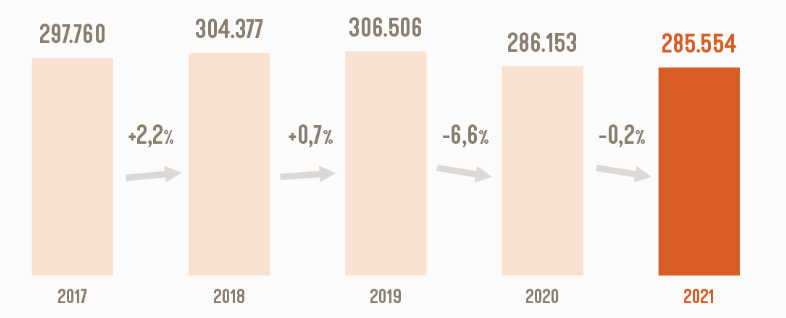
\includegraphics[width=0.5\textwidth]{imgs/grafica_abandonos.png}
    \caption{Gráfica de abandonos de animales en España en los últimos años. Fuente~\cite{affinity}}
    \label{fig:grafica_abandonos}
\end{figure}

Si bien es cierto que podemos observar en la gráfica que el número de animales abandonados ha disminuido en los últimos años, la situación no es tan
alentadora como parece. Los voluntarios de las protectoras y asociaciones de animales han tenido que hacer frente a la
situación de forma altruista para mantener el funcionamiento de las mismas, así como para atender a los animales que
llegan a sus instalaciones.

El paso del COVID ha agravado la situación, ya que muchas personas han tenido que abandonar a sus mascotas por no poder
prestarles atención y cuidarlas. El número de animales acogidos en los últimos años ha disminuido considerablemente, hasta el punto en el que
se ha establecido una etapa llamada generación COVID. \\

Es importante destacar que este problema no yace en la falta de voluntarios o iniciativas, sino en la falta de
concienciación y responsabilidad de la sociedad. Es necesario un compromiso de ciudadanos y autoridades para
apoyar y financiar a todos aquellos que realizan un esfuerzo de forma altruista para mejorar la situación de los
animales. \\

Actualmente, las protectoras y organizaciones se encuentran en una situación delicada y de saturación que genera un problema de
gestión en la información de los animales que acogen y buscan dar un nuevo hogar. A esto, se suma un
sector tecnológico que no ha prestado atención a este problema, ya que no le es rentable y no se encuentra
en su línea de negocio. \\


\section{Objetivos}\label{sec:objetivos}

Durante el desarrollo de este proyecto se han establecido una serie de objetivos que se deben cumplir de forma
progresiva. Estos objetivos se han establecido en función del tiempo de la asignatura, de las herramientas y los
conocimientos que se disponen y de las principales necesidades de las asociaciones y protectoras de animales: \\

\begin{enumerate}
    \item El principal objetivo es crear una \textbf{API} para la gestión de animales en adopción. Dentro de este gran objetivo,
    se puede hacer una subdivisión en los siguientes puntos a cumplir:
    \begin{itemize}
        \item Garantizar la seguridad de la información que circula entre la web, \textbf{API} y base de datos.
        \item Permitir a las organizaciones una gestión de la información de forma clara y sencilla.
        \item Permitir a los usuarios la adopción de un animal así como conocer el progreso y estado de las solicitudes.
        \item Permitir establecer un flujo de comunicación entre las organizaciones y los usuarios durante el proceso de adopción.
    \end{itemize}
    \item Crear una página web enfocada exclusivamente a las organizaciones que permita comprobar el correcto funcionamiento de la \textbf{API}.
    El diseño debe permitir una navegación clara y sencilla así como una gestión de la información rápida y eficiente.
    \item Aprender nuevos paradigmas de desarrollo de software y nuevas tecnologías.
    \item Identificar posibles mejoras y ampliaciones para el proyecto en futuros trabajos.
\end{enumerate}


\section{Metodología y herramientas}\label{sec:metodologia-y-herramientas-de-seguimiento}

Una vez definidos los objetivos del problema a resolver, en este apartado se explica la metodología y herramientas
utilizadas durante el desarrollo del proyecto.

\subsection{Metodología}\label{subsec:metodologia}

Para conseguir los objetivos propuestos, se ha seguido una metodología ágil en la que se ha diferenciado de forma
clara entre la creación de la \textbf{API}, la creación de la web y la propia documentación del proyecto. \\

La elección de la metodología ágil se debe a que permite adaptarse de forma rápida a cualquier cambio que pueda
surgir durante el desarrollo del proyecto y que además se basa en un trabajo incremental y continuo. Esto permite
que el proyecto se pueda llevar a cabo en un tiempo limitado, con una serie de tareas que se agrupan en
diferentes fases y que conforme se van completando de forma progresiva van añadiendo valor al producto final. \\

\begin{figure}[H]
\centering
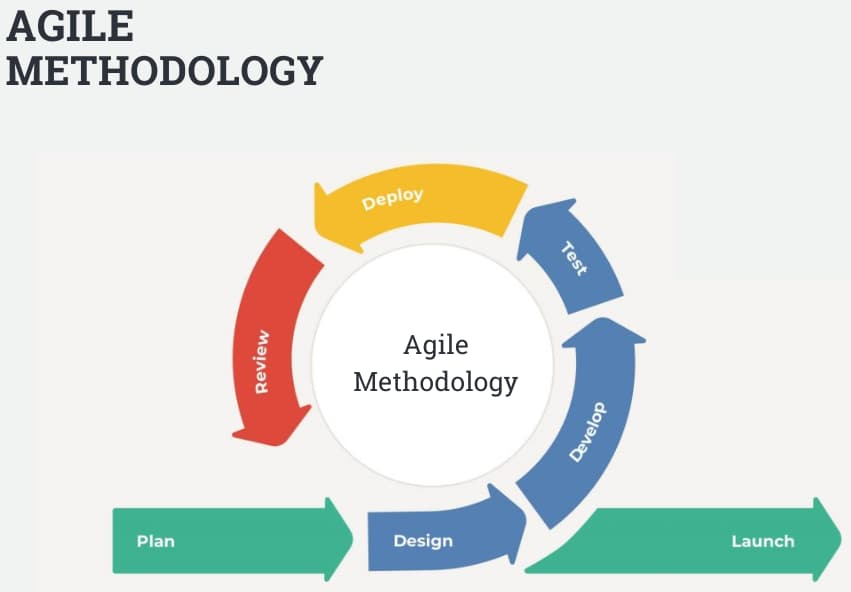
\includegraphics[width=0.5\textwidth]{imgs/metodologia_agil.jpg}
    \caption{Diagrama de la metodología ágil}
    \label{fig:metodologia_agil}
    \caption*{Fuente: \href{https://interqualitybg.com/en/resources/scrum-and-agile-resources/agile-methodology}{Interquality}}
\end{figure}

La metodología ágil que se ha utilizado en este proyecto es \textbf{Scrum}, ya que es una de las más populares en el
desarrollo de software actual, permite de una manera sencilla y ordenada llevar a cabo el desarrollo de un proyecto y
ofrece una gran flexibilidad a la hora de gestionar los cambios que puedan surgir en el proceso. \\

Si bien es verdad que el uso de estas técnicas se llevan a cabo en equipos con más integrantes y cuentan con
diferentes fases que priorizan la comunicación y colaboración en equipo, se ha decidido adaptar para que se pueda
llevar a cabo de forma individual sin dejar atrás los fundamentos y pilares de estas metodologías:

\begin{itemize}
    \item División del proyecto en diferentes fases compuestas por tareas (sprints).
    \item Contabilización de las horas invertidas en cada tarea y en el proyecto en general (medición del progreso).
    \item Fácil adaptación a posibles cambios.
    \item Trabajo incremental y continuo.
\end{itemize}

\subsection{Herramientas de seguimiento}\label{subsec:herramientas-de-seguimiento}

Para llevar a cabo los objetivos marcados por la metodología ágil, se han utilizado diferentes herramientas que
han permitido llevar un seguimiento del progreso del proyecto y de las tareas que se han ido completando
de una forma sencilla y ordenada. \\

Como gestión de control de versiones se ha utilizado \textbf{Git}. Esta herramienta permite el seguimiento de
cambios en el código así como la colaboración de diferentes personas que trabajen o quisieran colaborar en el
proyecto. Además, Git funciona de forma local y permite trabajar de forma offline, dando la posibilidad de
trabajar en cualquier momento y a cualquier hora. \\

Para alojar los proyectos, tanto de la \textbf{API} como de la web, se ha utilizado \textbf{GitHub}. Esta tecnología que
a diferencia de Git necesita de una conexión a internet para poder trabajar, permite el seguimiento y revisiones del
código, colaboración con otros usuarios y múltiples herramientas integradas que facilitan el desarrollo de software de
las cuales se han utilizado las siguientes:

\begin{itemize}
    \item \textbf{GitHub Actions}: permite la automatización de tareas y la integración continua.
    \item \textbf{GitHub Projects}: permite la creación de tableros de tareas y la gestión de los sprints.
    \item \textbf{GitHub Secrets}: permite la gestión de las variables de entorno de forma segura.
\end{itemize}

En los siguientes apartados se profundiza en cada una de estas herramientas y se explican sus usos en el proyecto.

\subsubsection{Historias de usuario (HU)}
GitHub permite la creación de tareas que pueden diferenciarse entre sí por medio de etiquetas clasificatorias o
por medio de una nomenclatura que permita identificarlas de forma rápida como por ejemplo \textbf{HU-1} para
la primera historia de usuario. \\

Las etiquetas que se han utilizado para diferenciar las tareas son las siguientes:

\begin{itemize}
    \item \textbf{task}: para señalar que se trata de una tarea.
    \item \textbf{bug}: para señalar que se trata de un error.
    \item \textbf{documentation}: para señalar que se trata de una tarea de documentación.
    \item \textbf{WIP}: para señalar que se trata de una tarea en progreso (Work In Progress).
    \item \textbf{HU}: para señalar que se trata de una historia de usuario.
    \item \textbf{don't merge}: para señalar que se trata de una tarea que no se debe mezclar con el resto del proyecto.
\end{itemize}

Una vez aclarado el uso de las etiquetas, se procede a explicar las diferentes historias de usuario que se han
desarrollado en el proyecto y que han tratado reflejar las necesidades de los usuarios y las organizaciones:

\begin{itemize}
    \item \textbf{HU-1: Como lector quiero poder conocer las bases del proyecto de manera clara y ordenada a partir de
    la memoria proporcionada}: esta historia de usuario es la asociada a la creación de la documentación del proyecto.
    \item \textbf{HU-2: Como organización quiero poder gestionar mis animales en adopción de manera sencilla}: esta
    historia de usuario cuenta con los siguientes criterios de aceptación:
        \begin{enumerate}
            \item Visualizar todos mis animales (perros/gatos)
            \item Añadir un nuevo animal
            \item Subir imágenes de los animales
            \item Borrar imágenes de los animales (antiguas, borrosas, etc.)
            \item Editar el perfil y los datos de mis animales
            \item Borrar animales que no estén disponibles para la adopción
            \item Visualizar las peticiones de mis animales por parte de los usuarios
            \item Aceptar o rechazar las peticiones de adopción de mis animales realizadas por los usuarios
        \end{enumerate}
    que han de ser cumplidos para que la historia de usuario se considere completada.
    \item \textbf{HU-3: Como organización quiero poder gestionar mi información personal}: esta historia de usuario cuenta
    con los siguientes criterios de aceptación:
        \begin{enumerate}
            \item Visualizar mi perfil
            \item Editar la información de mi perfil
            \item Subir imágenes a mi perfil
        \end{enumerate}
    que han de ser cumplidos para que la historia de usuario se considere completada.
    \item \textbf{HU-4: Como usuario quiero poder adoptar un animal}: esta historia de usuario cuenta con los siguientes
    criterios de aceptación:
        \begin{enumerate}
            \item Visualizar todos los animales disponibles para la adopción
            \item Visualizar los detalles de un animal dentro de una organización concreta
            \item Filtrar la búsqueda de animales con parámetros como raza, tamaño, sexo, etc.
            \item Solicitar la adopción de un animal
        \end{enumerate}
    que han de ser cumplidos para que la historia de usuario se considere completada.
    \item \textbf{HU-5: Como usuario quiero poder gestionar mi información personal}: esta historia de usuario cuenta
    con los siguientes criterios de aceptación:
        \begin{enumerate}
            \item Visualizar mi perfil
            \item Editar la información de mi perfil
            \item Subir imágenes a mi perfil
        \end{enumerate}
    que han de ser cumplidos para que la historia de usuario se considere completada.
\end{itemize}

Algunas de estas tareas y sus historias de usuario se pueden ver en la siguiente imagen:

\begin{figure}[H]
    \centering
    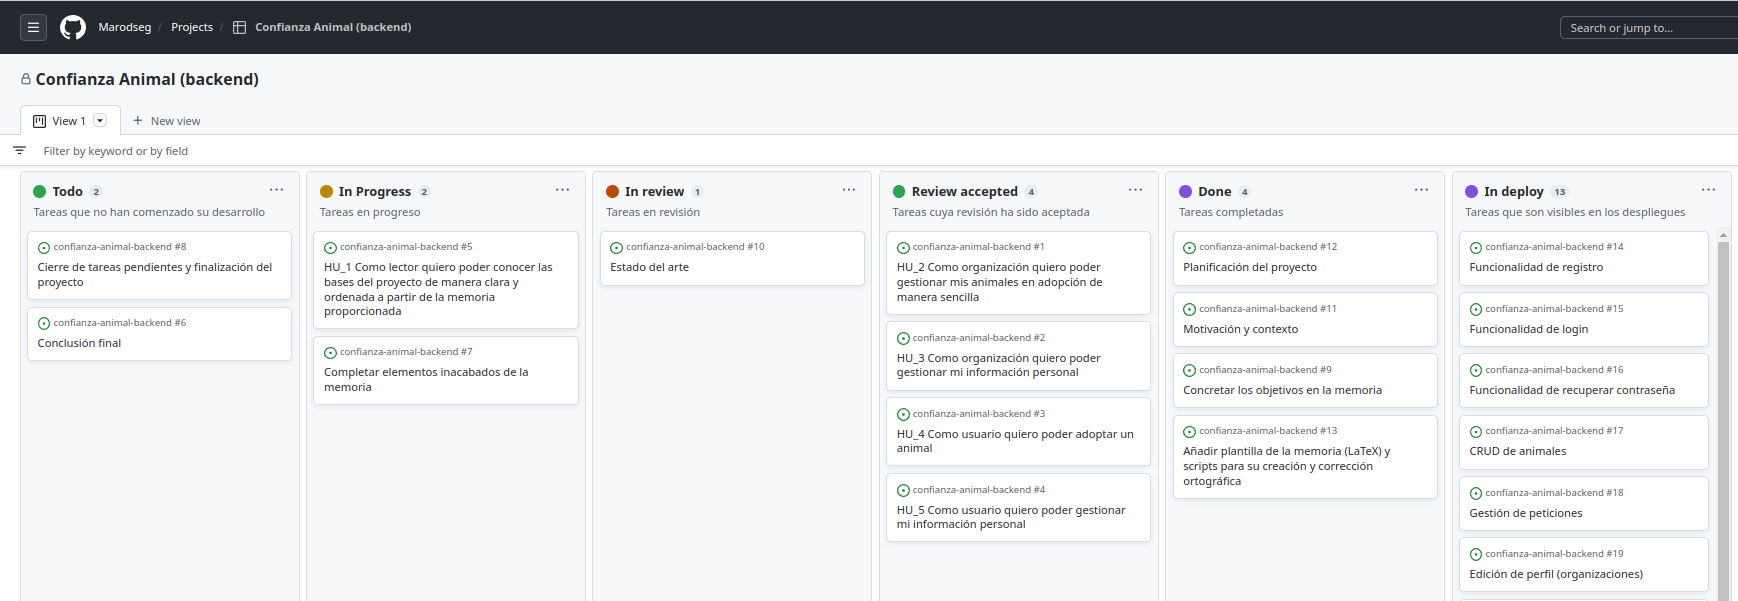
\includegraphics[width=0.9\textwidth]{imgs/tablero-github.png}
    \caption{Tablero de GitHub para el seguimiento de tareas}
    \label{fig:tablero-github}
\end{figure}

\subsubsection{Milestones}

El desarrollo del proyecto se ha dividido en \textit{milestones} (o hitos) que son entregables que marcan
el progreso del proyecto hacia la versión final. Son importantes para mantener un objetivo claro y tener una
forma de medir el éxito del producto a desarrollar. Los \textit{milestones} que se han llevado a cabo son los
siguientes:

\begin{enumerate}
    \item \textbf{Base e introducción}: engloba toda la preparación inicial del proyecto así como del entorno de
    trabajo. Además incluye los primeros pasos en la documentación, teniendo la historia de usuario \textbf{HU-1}
    mencionada anteriormente como objetivo principal de este hito.
    \item \textbf{Gestión de animales en adopción}: en este hito se recogen todos los objetivos relacionados con
    la administración de animales en una entidad de adopción (organización, perrera, asociación, etc.) y los
    usuarios que deseen adoptar alguno de ellos. Esto incluye
    la implementación de servicios que permitan a estas entidades gestionar sus animales, así como llevar un control
    de las peticiones de los usuarios por los mismos. Y servicios que permitan a los usuarios
    visualizar los animales y tener la posibilidad de notificar a la entidad su interés por alguno de ellos.
    \item \textbf{Conclusión}: en este hito se recogen todos los objetivos relacionados con la finalización del
    proyecto, incluyendo el cierre de tareas pendientes, finalización de la documentación y la entrega del proyecto.
\end{enumerate}

\begin{figure}[H]
    \centering
    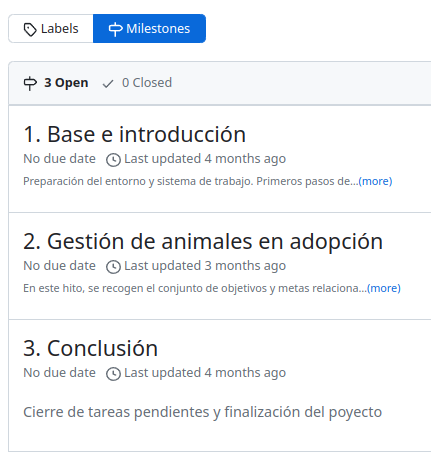
\includegraphics[width=0.5\textwidth]{imgs/milestones.png}
    \caption{Milestones del proyecto}
    \label{fig:milestones}
\end{figure}


\subsubsection{Integración continua}

La integración continua es una práctica llevada a cabo en el desarrollo de software que consiste en la ejecución
automática de pruebas y tareas de compilación cada vez que se realiza un cambio en el código fuente. De esta
forma se pueden detectar errores y permite corregirlos antes de que se produzca un fallo en el sistema. \\

Para llevar a cabo la integración continua se ha utilizado \textit{GitHub Actions}, un servicio que ofrece
GitHub para automatizar tareas en el repositorio. En este caso se ha utilizado para ejecutar diferentes pruebas
de calidad y testing de código así como el despliegue de la aplicación y la \textbf{API}:


\begin{itemize}
    \item \textbf{Estilo de código}: se ha utilizado \textit{Black} para comprobar el estilo de código de la
    \textbf{API} y \textit{Lint y Prettier} para la web. Estos servicios se ejecutan cada vez que se realiza un
    \textit{push} en cada repositorio y no permiten que se mezcle un código que no completa las pruebas con éxito.

    \newpage

    Se puede ver un ejemplo de la ejecución de estos servicios en las siguientes imágenes: \\

    \begin{figure}[H]
        \centering
        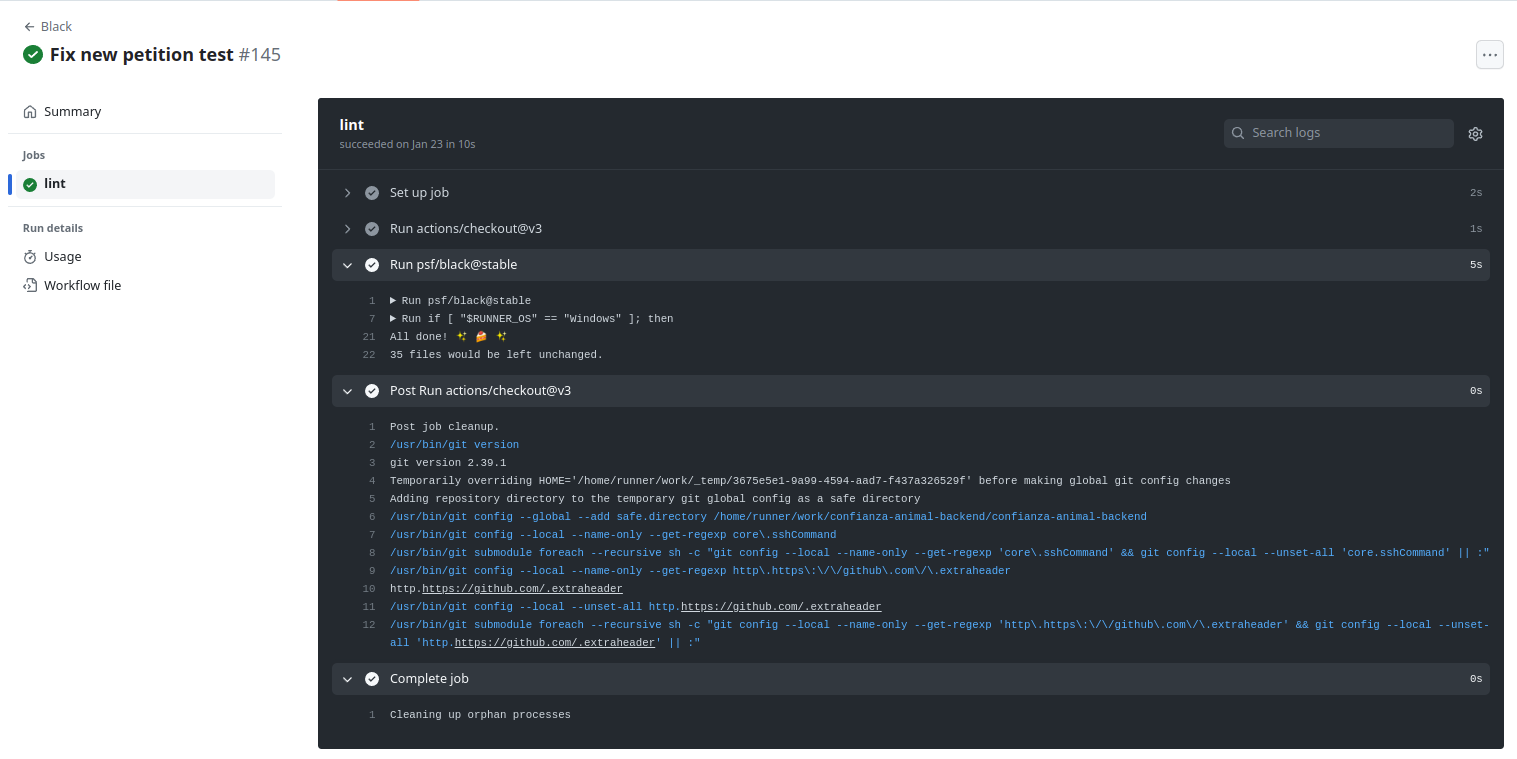
\includegraphics[width=0.9\textwidth]{imgs/black-action.png}
        \caption{GitHub Action Black en API}
        \label{fig:black-action}
    \end{figure}

    \begin{figure}[H]
        \centering
        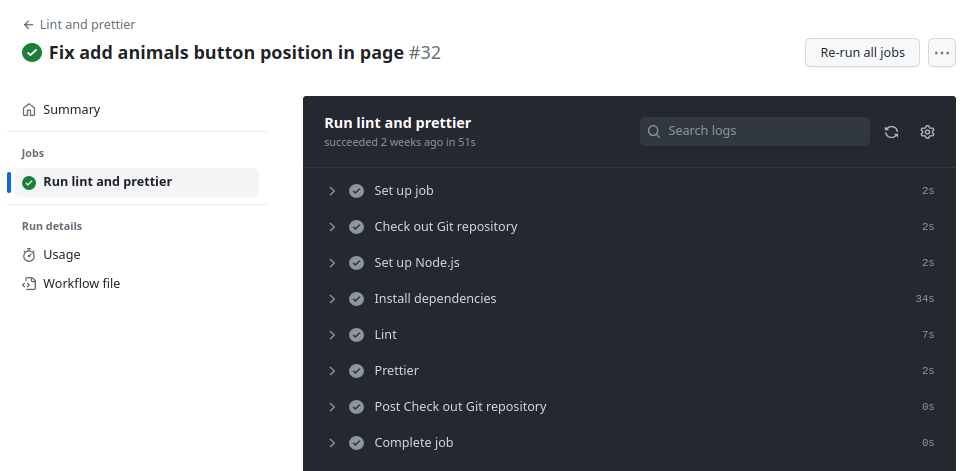
\includegraphics[width=0.9\textwidth]{imgs/lint-prettier-action.png}
        \caption{GitHub Action Lint y Prettier en Web}
        \label{fig:lint-prettier-action}
    \end{figure}

    \newpage

    \item \textbf{Testing}: se ha utilizado \textit{Pytest} para realizar las pruebas de la \textbf{API} y \textit{Karma} y
    \textit{Jasmine} para las pruebas de la web. Estos servicios se ejecutan cada vez que se realiza un
    \textit{push} en cada repositorio y no permiten que se mezcle el código con el resto si alguna de las pruebas falla.
    \item \textbf{Documentación}: para garantizar la calidad en la generación de este documento se ha utilizado un
    servicio que revisa la ortografía de cada cambio que se propone en el documento.
    \item \textbf{Despliegues}: se ha utilizado \textit{Render} para el despliegue de la API y \textit{Firebase Hosting} para
    el despliegue de la web. Estos servicios se ejecutan cada vez que se realiza un \textit{push} en cada repositorio
    sobre la rama principal y permiten el despliegue en un entorno de producción. En ambos repositorios se realiza
    una comprobación previa de que el código cumple con todas las pruebas mencionadas anteriormente para garantizar
    que los despliegues se realizan con éxito.
\end{itemize}



    \chapter{Planificación y presupuesto del proyecto}\label{ch:planificacion-y-presupuesto}

En esta sección se incluyen los aspectos relativos a la planificación del proyecto. Esta se divide en tres partes:
preparación inicial, desarrollo y conclusión. Cada una de estas partes representa una \textit{milestone} del proyecto
que se han realizado organizadas en \textit{sprints} de duración de dos semanas con el fin de poder llevar un control de las tareas realizadas
y alcanzar los objetivos previstos: \\

\textbf{Sprint 1: 1 de febrero - 14 de febrero}: preparación del proyecto. En este \textit{sprint} se abordan tareas únicamente
de la primera \textit{milestone}:

\begin{itemize}
    \item Creación de los repositorios
    \item Creación de la estructura inicial de los repositorios
    \item Creación de la estructura inicial de la memoria
\end{itemize}

\textbf{Sprint 2: 15 de febrero - 28 de febrero}: primeros pasos en la documentación. En este \textit{sprint} se pretende
avanzar en la documentación del proyecto de cara a cumplimentar la historia de usuario asociada a la primera \textit{milestone}:
\textbf{Como lector quiero poder conocer las bases del proyecto de manera clara y ordenada a partir de la documentación proporcionada}:
\begin{itemize}
    \item Motivación y contexto
    \item Estado del arte
\end{itemize}

\newpage

\textbf{Sprint 3: 1 de marzo - 14 de marzo}: requisitos del proyecto. En este \textit{sprint} se pretende establecer
los objetivos del proyecto una vez conociendo el contexto y el estado del arte y comenzar a definir los requisitos
del mismo:

\begin{itemize}
    \item Objetivos del proyecto
    \item Requisitos funcionales
    \item Requisitos no funcionales
\end{itemize}

\textbf{Sprint 4: 15 de marzo - 28 de marzo}: diseño del proyecto. En este \textit{sprint} se pretende comenzar a
diseñar el proyecto a partir de los requisitos establecidos en el \textit{sprint} anterior incluyendo las
tecnologías a utilizar:

\begin{itemize}
    \item Arquitectura del proyecto
    \item Diseño de la \textbf{API}
    \item Diseño de la base de datos
    \item Diseño de la aplicación web
\end{itemize}

\textbf{Sprint 5: 29 de marzo - 11 de abril}: implementación de la \textbf{API}. En este \textit{sprint} se pretende comenzar
con la implementación de la \textbf{API} y por tanto a cumplimentar diferentes tareas asociadas a la segunda \textit{milestone}:
\textbf{Gestión de animales en adopción}:

\begin{itemize}
    \item CRUD de animales
    \item CRUD de usuarios
    \item CRUD de organizaciones
    \item CRUD de peticiones de adopción
\end{itemize}

\textbf{Sprint 6: 12 de abril - 25 de abril}: implementación de la \textbf{API}. En este \textit{sprint} se pretende continuar
con la implementación de la \textbf{API}:

\begin{itemize}
    \item Registro y login de usuarios
    \item Registro y login de organizaciones
    \item Funcionalidad de reestablecimiento de contraseña
    \item Gestión de fotos de animales, usuarios y organizaciones
\end{itemize}

\textbf{Sprint 7: 26 de abril - 9 de mayo}: implementación de la \textbf{API}. En este \textit{sprint} se pretende finalizar
con la implementación de las tareas asociadas a la segunda \textit{milestone}:

\begin{itemize}
    \item Gestión de peticiones de adopción
    \item Visualización y filtrado de búsqueda de animales
\end{itemize}

\textbf{Sprint 8: 10 de mayo - 23 de mayo}: implementación de \textit{tests} y despliegues. En este \textit{sprint}
se pretende realizar la implementación de los \textit{tests} de la \textbf{API} y realizar el despliegue de la misma.

\textbf{Sprint 9: 24 de mayo - 6 de junio}: finalización de \textit{tests} e inicio de página web. En este \textit{sprint}
se pretende finalizar con la implementación de los \textit{tests} de la \textbf{API} y comenzar con la implementación de la página web.

\textbf{Sprint 10: 7 de junio - 20 de junio}: finalización de página web y despliegues. En este \textit{sprint} se pretende
dejar finalizados los despliegues de la \textbf{API} y la página web, comprobar su correcto funcionamiento y realizar los ajustes
necesarios. Se cierra a su vez la segunda \textit{milestone} del proyecto.

\textbf{Sprint 11: 21 de junio - 4 de julio}: finalización de la documentación y entrega del proyecto. En este \textit{sprint} se
pretende finalizar con la documentación del proyecto y realizar la entrega del mismo. Se cierra a su vez la tercera y
última \textit{milestone} del proyecto: \textbf{Conclusión}:

\begin{itemize}
    \item Cierre de tareas pendientes
    \item Conclusiones y finalización de la documentación
    \item Entrega del proyecto
\end{itemize}

\newpage

Durante los diferentes \textit{sprints} se han ido resolviendo las dudas presentadas con el tutor del proyecto
y se han completado los apartados correspondientes de la documentación en cada fase realizada. \\

En la siguiente tabla se muestra un resumen de las tareas en la
que se incluye el tiempo estimado para cada una de ellas:

\begin{table}[!ht]
  \centering
  \begin{tabular}{|l|l|}
    \hline
    \textbf{Tarea} & \textbf{Tiempo (horas)} \\
    \hline
    Planificación del proyecto & 90 \\
    Diseño de la API & 50 \\
    Implementación de la API & 150 \\
    Pruebas de la API & 50 \\
    Diseño de la página web & 20 \\
    Implementación de la página web & 50 \\
    Pruebas de la página web & 20 \\
    Diseño de la base de datos & 10 \\
    Pruebas de la base de datos & 20 \\
    Conclusiones & 10 \\
    \hline
    Total & 470 \\
    \hline
  \end{tabular}
  \caption{Planificación del proyecto}
  \label{tab:planificacion}
\end{table}

\newpage

\section{Diagrama de Gantt}\label{sec:diagrama-de-gantt}

El Diagrama de Gantt se usa para representar las tareas que se deben realizar en un proyecto, así como las fechas
en las que se deben realizar. En la siguiente figura se muestra el diagrama de Gantt del proyecto en el que, de forma
visual y clara, se puede ver la planificación de las tareas mencionadas anteriormente: \\

\begin{figure}[H]
    \centering
    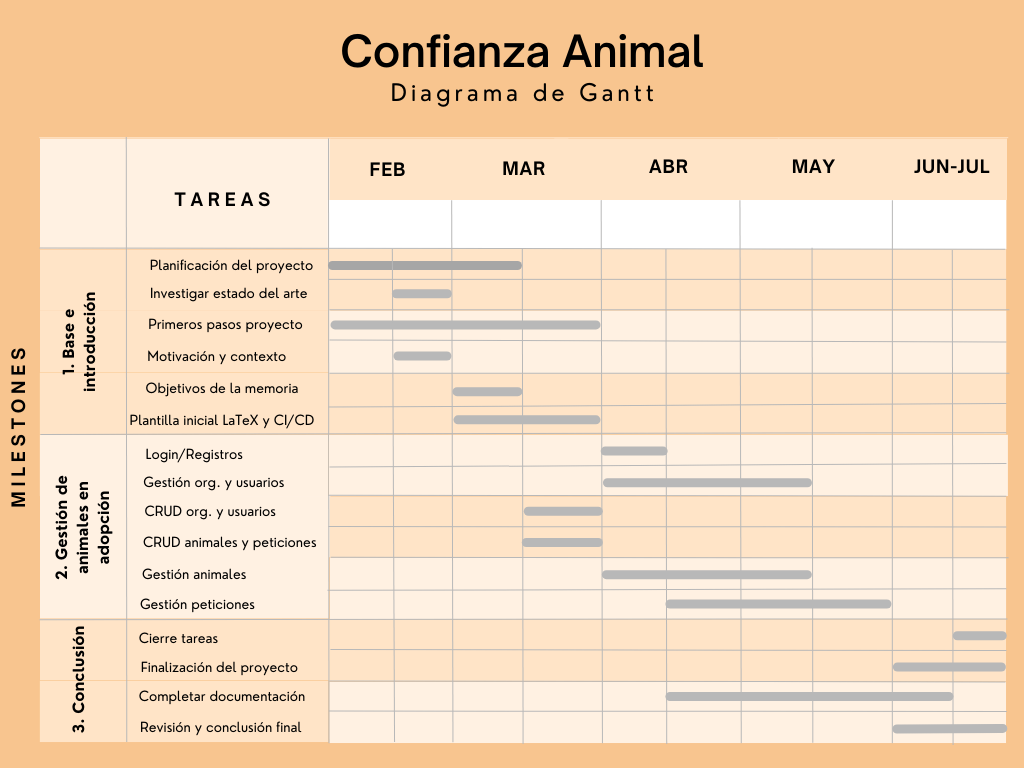
\includegraphics[width=\textwidth]{imgs/gantt}
    \caption{Diagrama de Gantt}
    \label{fig:diagrama-gantt}
\end{figure}

\newpage

\section{Elección de herramientas y tecnologías}\label{sec:eleccion-de-herramientas-y-tecnologias}

Antes de comenzar con el desarrollo del proyecto es necesario elegir las herramientas y tecnologías que se van a
utilizar para llevar a cabo el mismo. Para ello se han tenido en cuenta los requisitos del proyecto así como su
planificación y se ha llevado a cabo una investigación de las diferentes herramientas y tecnologías
existentes para cada una de las partes del proyecto que ha permitido elegir las más apropiadas para el desarrollo
del proyecto. Esto también nos ayudará a la hora de realizar la estimación de los costes del proyecto que se
explican en profundidad en la siguiente sección \ref{sec:presupuesto}.

\subsection{Framework web de API}\label{subsec:framework-web-de-api}

Para el desarrollo de la API se ha elegido \textbf{FastAPI}. Este framework por medio del lenguaje
de programación \textbf{Python} permite crear APIs de forma rápida y sencilla. Los motivos por los que
se ha elegido son los siguientes:

\begin{itemize}
    \item Es un framework moderno y rápido. El motivo de su alto rendimiento se debe a que hace uso de un sistema
    de tipado estático y un enfoque basado en declaraciones.
    \item Permite realizar operaciones de forma asíncrona. Gracias a la librería estándar \textbf{asyncio} permite que
    la API pueda realizar múltiples operaciones al mismo tiempo y de forma concurrente sin bloquear el hilo principal
    de ejecución dando una mayor velocidad de respuesta y escalabilidad.
    \item Permite realizar validaciones de datos. Por medio de la librería \textbf{Pydantic} se pueden
    validar y serializar los datos de forma automática aportando una mayor velocidad de ejecución y seguridad a la API.
    \item Permite realizar documentación de la API. FastAPI genera automáticamente una documentación interactiva
    basada en \textbf{OpenAPI} y \textbf{SwaggerUI} que facilita las pruebas de la API y la comprensión de la misma.
    \item Permite realizar la conexión con la base de datos. Uno de los puntos más importantes a la hora de elegir un
    framework es la facilidad de conexión con la base de datos. Debido a que su lenguaje de programación es \textbf{Python}
    y a día de hoy es uno de los lenguajes más utilizados en el mundo, la comunidad de desarrolladores ha creado
    una gran cantidad de librerías que permiten realizar conexiones con diferentes bases de datos. En este proyecto se ha
    usado la librería \textbf{Pyrebase}, que facilita la conexión con \textbf{Firebase} y permite realizar operaciones
    básicas como la autenticación, el almacenamiento de archivos, etc.
\end{itemize}

La gran cantidad de ventajas que ofrece \textbf{FastAPI} junto a su fácil aprendizaje sumado al interés personal
por aprender un nuevo framework hace que sea una de las mejores opciones para el desarrollo de este proyecto
frente a otras más comunes como pueden ser \textbf{Django} o \textbf{Flask}.

\subsection{Framework web de página web}\label{subsec:framework-web-de-pagina-web}

Para el desarrollo de la página web se ha elegido \textbf{Angular} en su versión 15 junto con \textbf{TypeScript}.
Angular es uno de los frameworks más utilizados en la actualidad para el desarrollo de aplicaciones web. Fue creado
por Google y su alta popularidad se debe a que es un framework muy robusto y escalable. Está basado en el patrón
de diseño \textbf{MVC} y permite realizar aplicaciones web de forma rápida y sencilla. \\

Pensando en el largo plazo, Angular es una de las mejores opciones posibles para el desarrollo de este proyecto. Cada 6 meses
Google aparece con una nueva versión que aporta nuevas características y mejoras, sigue una
arquitectura modular basada en componentes lo que proporciona una gran robustez, escalabilidad y mantenibilidad. El hecho
de que sea un framework de código abierto y que su comunidad sea muy activa hace que sea muy sencillo encontrar
soluciones a los problemas que se puedan presentar o componentes que se puedan reutilizar. \\

Angular necesita de un lenguaje de programación que se compile a JavaScript para poder
funcionar. En este proyecto se ha utilizado \textbf{TypeScript} ya que es un lenguaje que cumple con el requisito y además
tiene la peculiaridad de que es tipado estáticamente. Esto significa que el compilador de TypeScript comprueba que los
tipos de datos de las variables y funciones son correctos proporcionando así una mayor robustez y seguridad al código. \\

En los siguientes subapartados se mencionan en mayor profundidad los \textit{frameworks} CSS y bibliotecas empleadas que
han facilitado el diseño y creación de componentes de la página web como son \textbf{Angular Material}, \textbf{Bootstrap} y \textbf{Tailwind CSS}:

\subsubsection{Angular Material}\label{subsubsec:angular-material}

Angular Material es una biblioteca de componentes de diseño de código abierto para Angular que proporciona
una gran cantidad de componentes reutilizables y que ayudan a crear interfaces de usuario atractivas y funcionales. \\

Se basa en el diseño Material Design de Google, centrada en la simplicidad y la legibilidad. Entre su amplia gama de
componentes predefinidos se encuentran botones, barras de navegación, menús, listas, cuadros de diálogo, tablas, etc. \\

Algunas de las razones por las que se ha elegido Angular Material son:

\begin{itemize}
    \item \textbf{Responsive}: los componentes de Angular Material se adaptan a los diferentes tamaños de pantalla
    de forma automática y sin necesidad de escribir código adicional para ello.
    \item \textbf{Fácil de usar}: los componentes son muy fáciles de implementar y de usar ya que se basan en
    directivas de Angular y se pueden personalizar fácilmente mediante clases CSS y atributos.
    \item \textbf{Personalizable}: al ser código abierto, se puede ver el código fuente de los componentes y
    modificarlos a nuestro gusto para adaptarlos a nuestras necesidades.
    \item \textbf{Documentación}: la documentación de Angular Material es muy completa y detallada, además
    de que cuenta con ejemplos de uso de cada componente.
    \item \textbf{Accesibilidad}: los componentes de Angular Material cumplen con las normas de accesibilidad W3C~\cite{W3C} y
    están diseñados para que sean usados por personas con discapacidad visual, auditiva o motora.
\end{itemize}

\subsubsection{Bootstrap}\label{subsubsec:bootstrap}

Bootstrap es a día de hoy uno de los frameworks de CSS más populares y utilizados. Es un framework de código abierto
que permite la creación de interfaces de usuario \textit{responsive} por medio de componentes predefinidos, de
la misma forma que ocurre con Angular Material. \\

Usar Bootstrap junto a Angular Material ha permitido una serie de ventajas adicionales para el proyecto:

\begin{itemize}
    \item \textbf{Mayor variedad de componentes}: al combinar los componentes de Angular Material con los de Bootstrap,
    se ha conseguido una mayor variedad para la creación de las interfaces de usuario.
    \item \textbf{Ahorro de tiempo}: de la mano del punto anterior, el hecho de contar con un amplia gama de componentes predefinidos,
    se ha ahorrado tiempo en la creación de los componentes de la página web desde cero.
    \item \textbf{Compatibilidad}: Bootstrap asegura que sus componentes funcionan correctamente con los diferentes
    navegadores y dispositivos, lo cual garantiza una mayor experiencia de usuario y una interfaz más consistente.
    \item \textbf{Estilos por defecto}: Bootstrap cuenta con una gran cantidad de estilos CSS que permiten la personalización
    de los componentes de forma sencilla y rápida. Un ejemplo de esto podría ser la clase de estilo \texttt{mr-2} que
    añade automáticamente un margen a la derecha de 2 unidades a un elemento en vez de tener que escribir el código CSS correspondiente.
\end{itemize}

\subsubsection{Tailwind CSS}\label{subsubsec:tailwind-css}

Tailwind CSS es un framework de diseño web que se centra mayormente en proporcionar una amplia gama de clases CSS
personalizables para ayudar a crear interfaces de usuario de forma rápida y sencilla. A diferencia de Bootstrap, que
ya hemos viso que ofrece estilos predefinidos para los componentes, Tailwind CSS no proporciona ningún estilo por defecto,
sino que se basa en clases CSS que se pueden combinar para crear estilos personalizados. \\

Uno de los principales motivos por los que se ha añadido Tailwind CSS al proyecto es para probar un framework
moderno y que se está empezando a popularizar. Además, se ha elegido por su facilidad de uso, por la gran cantidad
de clases CSS que ofrece y por reducir las líneas de código CSS que se pueden llegar a escribir en un proyecto de
esta envergadura.

\subsection{Base de datos no relacional}\label{subsec:base-de-datos-no-relacional}

Para el almacenamiento de datos se ha elegido la base de datos de \textbf{Firebase}. Esta base de datos, tal y como
indica el apartado, es no relacional y se basa en colecciones y documentos. Cada documento es un objeto JSON que
contiene una serie de pares clave-valor. Los documentos se almacenan en colecciones que son como tablas en una base de datos
relacional. \\

Las bases de datos no relacionales, también conocidas como \textbf{NoSQL} se caracterizan por no tener que definir un
esquema de datos fijo previamente en el que se relacionen entre sí por medio de claves primarias o foráneas tal y
como ocurre en las bases de datos relacionales. Esto hace que las bases de datos no relacionales sean más flexibles
y escalables y no requieran de grandes consultas para obtener los datos. \\

Para este proyecto este tipo de base de datos es ideal ya que los animales pueden tener diferentes características
y sea necesario modificar el esquema de datos en cualquier momento. Además, se espera trabajar con una gran cantidad
de información e imágenes que requieren de un gran almacenamiento y para estos casos las bases de datos no relacionales
que escalan horizontalmente ofrecen un gran rendimiento en la lectura y escritura de datos. \\

En el siguiente subapartado se explicará con más detalle las características de \textbf{Firebase} y los motivos por
los que se ha elegido esta base de datos:

\subsubsection{Firebase}\label{subsubsec:firebase}
Firebase es una plataforma de Google que ofrece una amplia gama de servicios
para desarrollar aplicaciones web y móviles de una forma rápida, eficiente y de alta calidad. \\

La base de datos propia de Firebase es una base de datos no relacional que permite almacenar datos en forma de documentos JSON,
realizar consultas en tiempo real o añadir índices para mejorar la velocidad de las consultas. \\

No sólo se ha elegido Firebase para la base de datos, sino que también se ha elegido para el hosting de la
aplicación web del cual hablaremos más adelante en el capítulo~\ref{ch:implementacion-y-despliegues}, para la
autenticación de usuarios mediante el servicio de autenticación de Firebase, para la creación de notificaciones
push mediante el servicio de Cloud Messaging, para el almacenamiento de imágenes de los usuarios, organizaciones
y animales mediante el servicio de Cloud Storage y para la visualización de analíticas de la aplicación mediante
el servicio de Analytics. \\

Cabe señalar que la base de datos de Firebase permite la creación de reglas de seguridad que permiten controlar
el acceso a los datos de la base de datos. Estas reglas se pueden aplicar a la base de datos completa o a una
colección concreta. Además, se pueden aplicar reglas de seguridad a los documentos de la base de datos, de forma
que se puede controlar el acceso a los datos de forma más detallada. \\

Junto a estos motivos, se elige \textbf{Firebase} por ser una plataforma que se encuentra en la nube y al igual que pasa con Angular,
también es gestionada por Google lo cual nos da la seguridad de que los datos están protegidos y no tenemos que preocuparnos por la
gestión de servidores o la sincronización y comunicación entre herramientas. También ofrece una gran escalabilidad y
rendimiento de forma automática y permite la creación de índices dinámicos para mejorar la velocidad de las consultas
de una forma sencilla y rápida. Todo esto convierte \textbf{Firebase} como una herramienta ideal para el desarrollo
de este proyecto.

\section{Presupuesto}\label{sec:presupuesto}

A la hora de conformar un presupuesto para un proyecto se deben tener en cuenta los recursos que se necesitan para
llevar a cabo el mismo. Estos recursos pueden ser de diferente tipo como recursos humanos, recursos software o
recursos hardware:

\begin{itemize}
    \item \textbf{Recursos humanos}: son los costos asociados a los miembros del equipo de desarrollo. En este caso
    el equipo lo forma un único miembro, pero se han divido en diferentes roles para poder calcular el coste
    de cada uno de ellos.
    \item \textbf{Recursos software}: son los costos asociados a los recursos software que se necesitan en el proyecto
    como licencias, sistemas operativos, editores de código, etc.
    \item \textbf{Recursos hardware}: son los costos asociados a los recursos hardware que se necesitan en el proyecto
    como servidores, ordenadores, mantenimiento, etc.
\end{itemize}

\newpage

\subsection{Recursos humanos}\label{subsec:recursos-humanos}

Los recursos humanos necesarios para realizar el proyecto se muestran en la siguiente tabla: \\

\begin{table}[h]
    \centering
    \begin{tabular}{|l|l|l|l|}
        \hline
        \textbf{Rol} & \textbf{Precio por hora (€)} & \textbf{Tiempo (horas)} & \textbf{Coste total (€)} \\ \hline
        Manager & 100 & 130 & 13000 \\ \hline
        Programador & 80 & 300 & 24000 \\ \hline
        Diseñador & 60 & 10 & 600 \\ \hline
        QA Tester & 70 & 10 & 700 \\ \hline
        \hline
        \textbf{Total} & & 450 & 50000 \\ \hline
    \end{tabular}
    \caption{Recursos humanos}
    \label{tab:tabla_recursos_humanos}
\end{table}

\subsection{Recursos software}\label{subsec:recursos-software}

Los recursos software necesarios para realizar el proyecto se diferencian en dos tablas. La primera refleja
el coste personal que ha supuesto el proyecto y la segunda el coste real que supondría mantener el proyecto
en producción con sus correspondientes licencias. \\

\begin{table}[h]
    \centering
    \begin{tabular}{|l|c|}
        \hline
        \textbf{Recurso} & \textbf{Precio por mes (€)} \\ \hline
        Licencias de software & 0 \\ \hline
        Sistemas operativos & 0 \\ \hline
        Bibliotecas y frameworks & 0 \\ \hline
        Servidores & 0 \\ \hline
        Base de datos & 0 \\ \hline
        \hline
        \textbf{Total} & 0 \\ \hline
    \end{tabular}
    \caption{Recursos software}
    \label{tab:tabla_recursos_software_propios}
\end{table}

\begin{table}[h]
    \centering
    \begin{tabular}{|l|c|}
        \hline
        \textbf{Recurso} & \textbf{Precio por mes (€)} \\ \hline
        Licencias de software & 200 \\ \hline
        Sistemas operativos & 50 \\ \hline
        Bibliotecas y frameworks & 100 \\ \hline
        Servidores & 300 \\ \hline
        Base de datos & 100 \\ \hline
        \hline
        \textbf{Total} & 750 \\ \hline
    \end{tabular}
    \caption{Recursos software producción}
    \label{tab:tabla_recursos_software_producion}
\end{table}

\newpage

Como vemos en la primera tabla, el coste de los recursos software es de 0€ ya que se han utilizado herramientas
de código abierto y gratuitas. \\

Sin embargo, en la segunda tabla se reflejan precios que se tendrían que pagar si se quisiera mantener el proyecto
a nivel de producción. En este caso, se ha supuesto el precio licencias de software (programas de edición de imágenes,
editores de código, etc), el precio de los servidores (web y API) y el precio de la base de datos. Hay que tener en cuenta que
estos precios son orientativos y que pueden variar dependiendo de la necesidad de la aplicación. Si se necesitara
más capacidad de almacenamiento, más potencia en los servidores o más licencias de software, el precio aumentaría.

\subsection{Recursos hardware}\label{subsec:recursos-hardware}

Los recursos hardware necesarios para realizar el proyecto se muestran en la siguiente tabla: \\

\begin{table}[h]
    \centering
    \begin{tabular}{|l|l|c|c|c|}
        \hline
        \textbf{Recurso} & \textbf{Modelo} & \textbf{Coste (€)} & \textbf{Vida útil (años)} & \textbf{Amortización (€)} \\ \hline
        Ordenador & MSI GE63 Raider & 1700 & 6 & 283.33 \\ \hline
        \hline
        \textbf{Total} & & 1700 & &  283.33 \\ \hline
    \end{tabular}
    \caption{Recursos hardware}
    \label{tab:tabla_recursos_hardware}
\end{table}

A este presupuesto se le podrían añadir otros recursos hardware como un servidor web o un servidor de base de datos,
pero en este caso se ha optado por utilizar servicios en la nube que no requieren de un hardware específico para su
funcionamiento y que su precio se incluye en el apartado de recursos software.

\subsection{Presupuesto final}\label{subsec:presupuesto-final}

Para el cálculo del presupuesto final se ha tenido en cuenta el coste de los recursos humanos, software y hardware que
se han detallado en las tablas anteriores sin tener en cuenta el costo real que supondría mantener el proyecto en producción.
El resultado se muestra en la siguiente tabla: \\

\begin{table}[h]
    \centering
    \begin{tabular}{|l|c|c|}
        \hline
        \textbf{Recurso} & \textbf{Coste total (€)} \\ \hline
        Recursos humanos & 50000 \\ \hline
        Recursos software & 750/mes (producción) \\ \hline
        Recursos hardware & 1700 \\ \hline
        \hline
        \textbf{Total} & 51700 + 750/mes \\ \hline
    \end{tabular}
    \caption{Presupuesto final del proyecto}
    \label{tab:tabla_presupuesto_final}
\end{table}

    \chapter{Estado del arte}\label{ch:estado-del-arte}

En este apartado se analizará el estado del arte en el sector animal, más concretamente en la adopción de mascotas.
Primeramente se hará un análisis de las principales aplicaciones web que ofrecen la posibilidad de realizar
este proceso de forma interna y posteriormente se hará una conclusión en la que se justifique la necesidad de realizar
este trabajo.

\section{Miwuki Pet Shelter}\label{sec:miwuki}

\href{https://petshelter.miwuki.com/}{Miwuki} es una aplicación para facilitar el proceso de adopción de mascotas que
cuenta con la colaboración de la prestigiosa fundación Affinity. Además de contar con una versión móvil, tiene una
versión web que será la analizada a mayor profundidad en esta sección. \\

La web consiste en una página principal en la que se muestran las mascotas disponibles para su adopción así como
las diferentes protectoras que hay registradas en la aplicación. Gracias a una búsqueda personalizada se puede
encontrar la mascota que más se ajuste a las necesidades del usuario como por ejemplo el tamaño, la raza, el sexo,
la zona geográfica en España, etc. Además cuenta con una funcionalidad \textit{"Busca tu match!"} que permite encontrar
mascotas que se adapten a las características y estilo de vida del usuario, el cual necesitará estar registrado
en la aplicación. \\

Otra funcionalidad que ofrece es la posibilidad de dar en adopción una mascota con un límite máximo de 3 casos por cuenta.
Para ello, el usuario deberá registrarse en la aplicación y rellenar un formulario con los datos de la mascota para
publicitar el anuncio en la página principal. Además especifica que queda totalmente prohibida la venta y en caso de
detectar alguna publicación de este tipo, se procederá a su eliminación así como a la suspensión de la cuenta del
usuario. \\

Por último, podemos encontrar un apartado \textit{"Bolsa de pienso"} que redirige a una página que permite
realizar donaciones las cuales destinan el 90\% de su valor a las alimentos y el resto a los gastos de la
aplicación. \\

En la siguiente tabla se reflejan las características principales, ventajas y desventajas de la aplicación web
para tener una visión general de la misma: \\

\begin{table}[h]
\centering
\begin{tabular}{|p{6cm}|p{4cm}|p{4cm}|}
\hline
\textbf{Características principales} & \textbf{Pros} & \textbf{Contras} \\
\hline
Plataforma dedicada a la adopción de mascotas. &
Amplia variedad de animales para adoptar. &
Limitado a la adopción de mascotas. \\
\hline
Posibilidad de difundir la adopción de mascotas. &
Posibilidad de añadir a favoritos los animales que más te gusten. &
No existe un registro específico para las organizaciones. \\
\hline
Posibilidad de realizar donaciones. &
Posibilidad de dar en adopción una mascota. &
No existe un buscador de organizaciones. \\
\hline
\end{tabular}
\caption{Resumen de Miwuki Pet Shelter}
\label{tab:miwuki}
\end{table}


\section{Kerubi}\label{sec:kerubi}

\href{https://kerubi.es}{Kerubi} es una aplicación web para la adopción de mascotas. En su página principal se muestra
un buscador para encontrar el tipo de mascota que se desea adoptar (perros, gatos, conejos\ldots) y un seleccionador de
provincia. En la misma página en la parte inferior podemos ver los últimos animales que se han añadido a la aplicación
y tener la posibilidad de añadirlos a favoritos. \\

Los usuarios registrados tendrán la posibilidad de difundir la adopción de sus mascotas en la página principal por medio
de un formulario que deberá rellenar con los datos de la mascota. Además, los usuarios podrán realizar donaciones
para ayudar a las protectoras. \\

Por último, existe un registro específico para las organizaciones que deseen colaborar con la aplicación. En este caso,
las organizaciones deberán rellenar un formulario con los datos de la protectora y una vez aprobada, podrán publicar
los animales que deseen publicar en la web. \\

En la siguiente tabla se reflejan las características principales, ventajas y desventajas de la aplicación web
para tener una visión general de la misma: \\

\begin{table}[h]
\centering
\begin{tabular}{|p{6cm}|p{4cm}|p{4cm}|}
\hline
\textbf{Características principales} & \textbf{Pros} & \textbf{Contras} \\
\hline
Plataforma de adopción y difusión de mascotas. &
Amplia variedad de animales para adoptar. &
Algunas funcionalidades requieren registro. \\
\hline
Contacto con criadores y particulares. &
Opciones de adopción y difusión de mascotas. &
Falta de control en la gestión de adopción. \\
\hline
Amplio catálogo de animales. &
Posibilidad de encontrar razas específicas. &
Costos adicionales asociados a la adopción. \\
\hline
Funcionalidad de búsqueda avanzada con filtros personalizables. &
Interfaz intuitiva y fácil de usar. &
Exceso de publicidad en la plataforma. \\
\hline
\end{tabular}
\caption{Resumen de Kerubi}
\label{tab:kerubi}
\end{table}

\section{Kiwoko adopta}\label{sec:kiwoko}

\href{https://kiwokoadopta.org}{Kiwoko} es una aplicación web para la adopción de mascotas. En su página principal se muestra
una lista de enlaces con búsquedas rápidas como "Perros en Granada" o "Roedores en Albacete", un buscador para encontrar
el tipo de mascota que se desea adoptar (perros, gatos o roedores) y un seleccionador de tamaño, edad y provincia.
También se ven algunos resultados por defectos que van cambiando según se vayan realizando búsquedas. \\

Kiwoko se encarga de verificar que las organizaciones que se dan de alta en la plataforma cumplan con los requisitos
legales y consten como una protectora de animales oficial. Una vez verificadas, podrán publicar los animales que
deseen en la web. \\

En esta ocasión no contamos con una funcionalidad para que los usuarios puedan difundir la adopción de sus mascotas,
ni tampoco con la opción de añadir a favoritos los animales por los que más estés interesado. Esto permite
que los anuncios que aparecen en la web sean de organizaciones y no de particulares y cuenten con la verificación
de la aplicación. \\

En la siguiente tabla se reflejan las características principales, ventajas y desventajas de la aplicación web
para tener una visión general de la misma: \\

\begin{table}[h]
\centering
\begin{tabular}{|p{6cm}|p{4cm}|p{4cm}|}
\hline
\textbf{Características principales} & \textbf{Pros} & \textbf{Contras} \\
\hline
Plataforma dedicada a la adopción de mascotas. &
Amplia variedad de animales para adoptar. &
Funcionalidades limitadas. \\
\hline
Gran cantidad de detalles de cada animal en adopción. &
Alta verificación de las organizaciones. &
Interfaz con un diseño poco atractivo. \\
\hline
Posibilidad de búsqueda por ubicación y categoría de animales. &
Facilidad para contactar directamente con las organizaciones. &
Falta de añadir a favoritos los animales que más te gusten. \\
\hline
Enlace a la web de la organización para más información. &
Registro de organizaciones verificado. &
Falta de información actualizada sobre animales disponibles. \\
\hline
\end{tabular}
\caption{Resumen de Kiwoko Adopta}
\label{tab:kiwoko-adopta}
\end{table}


\section{Mascostas adopción}\label{sec:mascostas}

\href{https://mascotasadopcion.com}{Mascostas adopción} es una aplicación web sencilla para la adopción de mascotas.
A diferencia de las ya mencionadas anteriormente, esta aplicación no requiere de un registro para poder adoptar una
mascota. En su página principal se muestran las mascotas disponibles para su adopción y un buscador de provincia,
animal y sexo. Si estás interesado por un animal, puedes rellenar un formulario con datos personales y de contacto
para que la protectora se ponga en contacto contigo y avanzar en el proceso de adopción. \\

En caso de estar registrado como usuario, puedes añadir a favoritos los animales que más te gusten y así poder
tener un acceso más rápido a ellos. Además, puedes realizar donaciones para ayudar a las protectoras, ver los animales
que ya han sido adoptados o difundir la adopción de tus mascotas. \\

En esta aplicación no contamos con el rol de organización, por lo que los anuncios que aparecen en la web son
de particulares y no se puede garantizar que todos los animales que se publican sean reales o que cumplan con las
condiciones legales para su adopción. \\

En la siguiente tabla se reflejan las características principales, ventajas y desventajas de la aplicación web
para tener una visión general de la misma: \\

\begin{table}[h]
\centering
\begin{tabular}{|p{6cm}|p{4cm}|p{4cm}|}
\hline
\textbf{Características principales} & \textbf{Pros} & \textbf{Contras} \\
\hline
Plataforma dedicada a la adopción de mascotas. &
Amplia variedad de animales para adoptar. &
Falta de control en el proceso de adopción. \\
\hline
Posibilidad de búsqueda por ubicación y categoría de animales. &
Interfaz intuitiva, moderna y fácil de usar. &
Costos adicionales asociados a la adopción. \\
\hline
Posibilidad de difundir la adopción de mascotas. &
Posibilidad de realizar donaciones. &
Falta de filtrado de organizaciones. \\
\hline
Posibilidad de añadir a favoritos los animales que más te gusten. &
Posibilidad de ver los animales que ya han sido adoptados. &
Falta de información actualizada sobre animales disponibles. \\
\hline
\end{tabular}
\caption{Resumen de Mascostas en adopción}
\label{tab:mascotas-adopcion}
\end{table}

\section{Webs de protectoras y ayuntamientos}\label{sec:protectoras-ayuntamientos}

Además de las aplicaciones web que hemos analizado anteriormente, existen otras webs que ofrecen la posibilidad
de realizar la adopción de mascotas por medio de formularios en vez de en la propia aplicación. Estas webs
suelen ser de protectoras de animales o de ayuntamientos y suelen tener un diseño más sencillo que las aplicaciones
mencionadas anteriormente. Su objetivo es fomentar y difundir la adopción de animales pero debido a la falta de
interacción con los usuarios y de los bajos recursos que tienen, no suelen ser muy utilizadas. \\

Ejemplo de estas webs son:

\begin{itemize}
    \item \href{https://www.lasrozas.es/sanidad-y-servicios-sociales/adoptar-animales}{Ayuntamiento de Las Rozas}
    \item \href{https://csmpa.palma.cat/portal/PALMA/csmpa/contenedor1.jsp?seccion=s_fdes_d4_v1.jsp&codbusqueda=1720&language=es&codResi=1&layout=contenedor1.jsp&codAdirecto=981}{Ajuntament de Palma}
    \item \href{https://www.valladolid.es/es/programa-adopta}{Ayuntamiento de Valladolid}
    \item \href{https://protectorabcn.es/adopta/}{Protectora de Barcelona}
    \item \href{https://elrefugio.org/adopta/}{El Refugio}
    \item \href{https://nuevavida-adopciones.org/}{Nueva Vida Adopciones}
    \item \href{https://www.anaaweb.org/}{Asociación Nacional de Amigos de los Animales}
\end{itemize}

En la siguiente tabla se reflejan las características principales, ventajas y desventajas de este tipo de webs
para tener una visión general de las mismas: \\

\begin{table}[h]
\centering
\begin{tabular}{|p{6cm}|p{4cm}|p{4cm}|}
\hline
\textbf{Características principales} & \textbf{Pros} & \textbf{Contras} \\
\hline
Plataformas informativas sobre la adopción de mascotas. &
Amplia variedad de información de animales en adopción. &
Falta de posibilidad de adopción. \\
\hline
Posibilidad de búsqueda por ubicación y categoría de animales. &
Amplia variedad de información sobre protectoras. &
Interfaces poco atractivas y poco intuitivas. \\
\hline
Posibilidad de difundir la adopción de mascotas. &
Posibilidad de realizar donaciones. &
Falta de filtrado de organizaciones. \\
\hline
Toda la información se encuentra actualizada. &
Posibilidad de ver los animales que ya han sido adoptados. &
Fallos de seguridad. \\
\hline
\end{tabular}
\caption{Resumen de webs de protectoras y ayuntamientos}
\label{tab:protectoras-ayuntamientos}
\end{table}

\section{Conclusiones}\label{sec:conclusiones-estado-del-arte}

Una vez analizadas las principales aplicaciones web para la adopción de mascotas, podemos concluir que ninguna de las
mencionadas cuenta con una web privada para las organizaciones con el fin de ayudarlas a gestionar
toda la información con la que tratan y que se genera a diario. Además, ninguna de las aplicaciones permite la
gestión de las peticiones que se realizan a través de las mismas, por lo que las organizaciones no pueden mantener
una comunicación fluida con los usuarios que desean adoptar una mascota. También cabe destacar que algunas de las
webs no cuentan con un diseño atractivo y moderno, lo que puede provocar que los usuarios no se sientan atraídos
por la aplicación y no la utilicen sumando a esto la falta de información actualizada sobre los animales disponibles
para la adopción y en algunos casos la imposibilidad de realizar la adopción a través de la propia aplicación. \\

En este proyecto se pretende desarrollar una API que permita a las organizaciones gestionar toda la información
pertinente a su actividad y que les ayude a controlar todas las peticiones que se realizan a través de la aplicación, es
decir, crear un flujo de comunicación entre las organizaciones y los usuarios que deseen adoptar una mascota a través
de diferentes estados de la petición con información relevante para ambos y con mensajes que permitan mantener
una comunicación fluida y actualizada. \\

La página web que se desarrollará para el proyecto contará con una interfaz de usuario que permita a las organizaciones
un control claro y sencillo de toda la información y de las peticiones que se realicen a través de la aplicación móvil
que se encargará de desarrollar mi compañero de proyecto Alejandro y que haciendo uso de la API, implementará todas
las funcionalidades haciendo hincapié en mejorar los defectos que hemos encontrado en las aplicaciones analizadas
anteriormente. \\

    \chapter{Análisis del problema}\label{ch:analisis-del-problema}

Para realizar cualquier proyecto de Ingeniería del Software es necesario llevar a cabo un análisis del problema,
en el que se definen los requisitos del sistema, se describen los actores que interactúan con el sistema y se
realizan los diagramas de caso de uso. El objetivo es conseguir un producto que cumpla con los requisitos y
necesidades que requiere el cliente.

\section{Ingeniería de requisitos}\label{sec:ingenieria-de-requisitos}

La ingeniería de requisitos consiste en la definición delos requisitos del sistema, es decir, las características
que debe tener el sistema para que sea aceptado por el cliente. Durante esta fase se llevan a cabo una serie
de actividades que permiten obtener un producto de calidad:

\begin{itemize}
    \item \textbf{Identificación de requisitos}: se recopila información sobre el sistema y se identifican
    las necesidades de usuarios, organizaciones y partes interesadas.
    \item \textbf{Análisis de requisitos}: se realiza una descripción detallada de los requisitos del sistema,
    se definen los casos de uso y se identifican los actores que interactúan con el sistema así como los
    requisitos funcionales y no funcionales.
    \item \textbf{Viabilidad del sistema}: se comprueba que el sistema es viable, es decir, que se pueda
    desarrollar cumpliendo los requisitos y se comprueba que estos sean consistentes, completos y no contradictorios.
\end{itemize}

\newpage

\subsection{Requisitos funcionales}\label{subsec:requisitos-funcionales}

Los requisitos funcionales son aquellos que definen las funciones que debe realizar el sistema. Describen la
interacción entre el sistema y el usuario, es decir, lo que el usuario puede hacer con el sistema. En este caso,
a pesar de tener como actores a los usuarios y a la organización, los requisitos funcionales se centran en
las funciones que puede realizar la organización ya que es la que va a utilizar el sistema que se va a desarrollar.
Los requisitos referidos a los usuarios se describen en la aplicación móvil que desarrollará mi compañero de
trabajo.

\begin{itemize}
    \item \textbf{RF-1.} Gestión de la organización
    \begin{itemize}
        \item \textbf{RF-1.1.} Alta de organización
        \item \textbf{RF-1.2.} Subir foto de perfil
        \item \textbf{RF-1.3.} Modificar información de la organización
        \item \textbf{RF-1.4.} Recuperar contraseña
        \item \textbf{RF-1.5.} Desactivar cuenta
        \item \textbf{RF-1.6.} Activar cuenta
    \end{itemize}
    \item \textbf{RF-2.} Gestión de animales
    \begin{itemize}
        \item \textbf{RF-2.1.} Alta de animales
        \item \textbf{RF-2.2.} Baja de animales
        \item \textbf{RF-2.3.} Modificación de la información de los animales
        \item \textbf{RF-2.4.} Subir fotos de los animales
        \item \textbf{RF-2.5.} Eliminar fotos de los animales
    \end{itemize}
    \item \textbf{RF-3.} Gestión de peticiones
    \begin{itemize}
        \item \textbf{RF-3.1.} Actualizar estado
        \item \textbf{RF-3.2.} Aprobar información del usuario
        \item \textbf{RF-3.3.} Rechazar información del usuario
        \item \textbf{RF-3.4.} Aprobar documentación del usuario
        \item \textbf{RF-3.5.} Rechazar documentación del usuario
        \item \textbf{RF-3.6.} Aprobar petición
        \item \textbf{RF-3.7.} Rechazar petición
    \end{itemize}
\end{itemize}

\subsection{Requisitos no funcionales}\label{subsec:requisitos-no-funcionales}

Los requisitos no funcionales son aquellos que describen las restricciones o características que debe cumplir el
sistema. A diferencia de los funcionales, estos requisitos no se centran en las funciones que debe realizar el sistema.

\begin{table}[H]
    \centering
    \begin {tabular} {| l | l |}
        \hline
        \textbf {RFN-1}
        & \underline{Usabilidad} \\
        & \tabitem El sistema debe ser fácil de usar \\
        & \tabitem El sistema debe ser intuitivo \\
        \hline

        \textbf {RFN-2}
        & \underline{Seguridad} \\
        & \tabitem El sistema debe tener un sistema de autenticación \\
        & \tabitem El sistema debe tener un sistema de verificación de la identidad \\
        & \tabitem El sistema debe proteger la información de los usuarios y organizaciones \\
        \hline

        \textbf {RFN-3}
        & \underline{Fiabilidad} \\
        & \tabitem El sistema debe ser resistente a fallos \\
        & \tabitem El sistema debe ser resistente a ataques externos \\
        \hline

        \textbf {RFN-4}
        & \underline{Rendimiento} \\
        & \tabitem El sistema debe ser rápido \\
        & \tabitem El sistema debe ser escalable \\
        \hline

        \textbf {RFN-5}
        & \underline{Eficiencia} \\
        & \tabitem El sistema debe ser eficiente en el uso de los recursos \\
        & \tabitem El sistema debe ser capaz de soportar un gran número de usuarios \\
        & \tabitem El sistema debe ser capaz de soportar un gran número de peticiones \\
        & \tabitem El sistema debe ser capaz de soportar un gran número de animales \\
        & \tabitem El sistema debe ser capaz de soportar un gran número de imágenes \\
        \hline

        \textbf {RFN-6}
        & \underline{Compatibilidad} \\
        & \tabitem El sistema debe ser compatible con los navegadores más utilizados \\
        & \tabitem El sistema debe ser compatible con los dispositivos más utilizados \\
        \hline

        \textbf {RFN-7}
        & \underline{Disponibilidad} \\
        & \tabitem El sistema debe estar disponible el mayor tiempo posible \\
        \hline

        \textbf {RFN-8}
        & \underline{Mantenibilidad} \\
        & \tabitem El sistema debe ser fácil de mantener \\
        & \tabitem El sistema debe ser fácil de actualizar \\
        \hline

        \textbf {RFN-9}
        & \underline{Ética} \\
        & \tabitem El sistema debe cumplir con la normativa vigente de protección de datos \\
        & \tabitem El sistema debe cumplir con la normativa vigente de protección de animales \\
        \hline

    \end {tabular}
    \caption {Requisitos no funcionales}
    \label {tab:requisitos-no-funcionales}
\end {table}

\newpage

\subsection{Requisitos de información}\label{subsec:requisitos-de-informacion}

Los requisitos de información son aquellos que describen la información que debe almacenar el sistema (aplicación web).

\begin{table}[H]
    \centering
    \begin {tabular} {| l | l |}
        \hline
        \textbf {RI-1}
        & \underline{Organizaciones} \\
        & \tabitem Información para el registro en la aplicación \\
        & \tabitem Información de contacto: nombre, teléfono, email, foto de perfil, dirección\ldots \\
        & \textbf{Requisitos funcionales:} RF-2. \\
        \hline

        \textbf {RI-2}
        & \underline{Usuarios} \\
        & \tabitem Información para el registro en la aplicación \\
        & \tabitem Información de contacto: nombre, teléfono, email, foto de perfil, dirección\ldots \\
        & \tabitem Información de las mascotas guardadas en favoritos \\
        & \tabitem Información de las peticiones realizadas \\
        \hline

        \textbf {RI-3}
        & \underline{Animales} \\
        & \tabitem Información del animal: nombre, raza, edad, sexo, tamaño\ldots \\
        & \tabitem Imágenes del animal \\
        & \textbf{Requisitos funcionales:} RF-1. \\
        \hline

        \textbf {RI-4}
        & \underline{Peticiones} \\
        & \tabitem Información de la petición: animal, descripción, fecha de creación, estado\ldots \\
        & \textbf{Requisitos funcionales:} RF-3. \\
        \hline

    \end {tabular}
    \caption {Requisitos de información}
    \label {tab:requisitos-informacion}
\end {table}

\newpage

\section{Descripción de actores}\label{sec:descripcion-de-actores}

Los actores son los elementos que interactúan con el sistema. En este caso, los actores son las organizaciones y los usuarios.
También existe un actor \textbf{admin} que es el encargado de gestionar la aplicación pero no interactúa con ella directamente.
No se ha considerado como un actor externo ya que coincide con el propio desarrollador del proyecto y se obvia que
tiene todos los privilegios sobre la aplicación y la base de datos y por tanto puede realizar cualquier acción.

En la siguiente tabla se describe únicamente la información relevante a la organización ya que el usuario no
pertenece a la aplicación web, sino que participa en la aplicación móvil y no tiene información relevante para esta
documentación.


\subsection{Organización}\label{subsec:organizacion}

\begin{table}[H]
\begin{center}
    \begin{adjustbox}{width=\textwidth}
    \begin{tabular}{ | l | l | l | l | c | c | }
        \hline
        \textbf{Actor} & \multicolumn{4}{l|}{Organización} & \cellcolor{gray!50} \textbf{ACT-1}\\
        \hline
        \textbf{Descripción} & \multicolumn{5}{p{0.9\linewidth}|}{Representa a una
        organización que se registra en la aplicación (asociación, protectora, refugio\ldots).} \\
        \hline
        \textbf{Características} & \multicolumn{5}{p{0.5\linewidth}|}{Está registrada
        en el sistema y por tanto puede publicar animales y gestionar la información de los animales y las peticiones.} \\
        \hline
        \textbf{Relaciones} & \multicolumn{5}{p{0.5\linewidth}|}{ } \\
        \hline
        \textbf{Referencias} & \multicolumn{5}{p{0.5\linewidth}|}{CU-1.1, CU-1.2, CU-1.3, CU-1.4, CU-1.5, CU-1.6,
        CU-2.1, CU-2.2, CU-2.3, CU-2.4, CU-2.5, CU-3.1, CU-3.2, CU-3.3, CU-3.4, CU-3.5, CU-3.6, CU-3.7 } \\
        \hline
        \textbf{Autor} & \multicolumn{1}{p{0.25\linewidth}|}{Manuel Ángel Rodríguez Segura} & \textbf{Fecha} &
        08-04-2023     & \textbf{Versión}                                                      & 1.0\\
        \hline
    \end{tabular}
    \end{adjustbox}
    \caption{Actor: Organización}
    \label{tab:organizacion}
\end{center}
\end{table}

\newpage

\section{Diagramas de Caso de Uso}\label{sec:diagramas-de-caso-de-uso}

Los diagramas de caso de uso son una representación gráfica que nos permite visualizar los actores y las acciones que
pueden realizar sobre el sistema. En el desarrollo de software son una herramienta muy útil para la comunicación entre
el cliente y el desarrollador ya que permiten mostrar de forma sencilla las funcionalidades del sistema. \\

Para la realización de los diagramas de caso de uso se ha utilizado la herramienta de Google \textbf{draw.io}.
A continuación se muestran los diferentes diagramas involucrados en el sistema:

\subsection{Gestión de organización}\label{subsec:gestion-de-organizacion}

\begin{figure}[H]
    \centering
    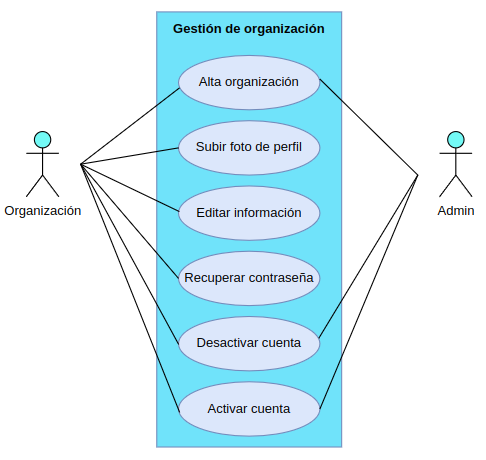
\includegraphics[width=0.8\textwidth]{imgs/gestion-organizacion}
    \caption{Gestión de organización}
    \label{fig:diagrama-caso-uso-gestion-organizacion}
\end{figure}

\subsubsection{Caso de Uso 1.1: Alta organización}\label{subsubsec:alta-organizacion}

\begin{table}[H]
    \begin{center}
        \begin{adjustbox}{width=\textwidth}
            \begin{tabular}{ | l | l | l | l | c | c | }
                \hline
                \textbf{Caso de uso} & \multicolumn{4}{l|}{Alta organización} & \cellcolor{gray!50} \textbf{CU-1.1}\\
                \hline
                \textbf{Actores} & \multicolumn{5}{p{0.5\linewidth}|}{Organización, admin} \\
                \hline
                \textbf{Tipo} & \multicolumn{5}{l|}{Primario y esencial} \\
                \hline
                \textbf{Referencias} & \multicolumn{3}{l|}{RF-1.1} & \multicolumn{2}{l|}{ }\\
                \hline
                \textbf{Precondición} & \multicolumn{5}{l|}{La organización no puede estar registrada previamente} \\
                \hline
                \textbf{Postcondición} & \multicolumn{5}{l|}{La organización es registrada y puede usar la aplicación en su totalidad} \\
                \hline
                \textbf{Autor} & \multicolumn{1}{p{0.25\linewidth}|}{Manuel Ángel Rodríguez Segura} & \textbf{Fecha} &
                08-04-2023     & \textbf{Versión}                                                      & 1.0\\
                \hline
            \end{tabular}
        \end{adjustbox}
        \caption{CU-1.1: Alta organización}
        \label{tab:alta-organizacion}
    \end{center}
\end{table}

\begin{table}[H]
    \centering
    \begin{tabularx}{\textwidth}{@{} |L |@{}} \hline
        \rowcolor{gray!50}
        \textbf{Propósito} \\
        \hline
        Permite a una organización registrarse en el sistema. \\
        \hline
    \end{tabularx}
\end{table}

\begin{table}[H]
    \centering
    \begin{tabularx}{\textwidth}{@{} |L |@{}} \hline
        \rowcolor{gray!50}
        \textbf{Resumen} \\
        \hline
        Permite a una organización registrarse en el sistema y acceder a todas las funcionalidades de la aplicación. \\
        \hline
    \end{tabularx}
\end{table}

\subsubsection{Caso de Uso 1.2: Subir foto de perfil}\label{subsubsec:subir-foto-perfil}

\begin{table}[H]
    \begin{center}
        \begin{adjustbox}{width=\textwidth}
            \begin{tabular}{ | l | l | l | l | c | c | }
                \hline
                \textbf{Caso de uso} & \multicolumn{4}{l|}{Subir foto de perfil} & \cellcolor{gray!50} \textbf{CU-1.2}\\
                \hline
                \textbf{Actores} & \multicolumn{5}{p{0.5\linewidth}|}{Organización} \\
                \hline
                \textbf{Tipo} & \multicolumn{5}{l|}{Primario y esencial} \\
                \hline
                \textbf{Referencias} & \multicolumn{3}{l|}{RF-1.2} & \multicolumn{2}{l|}{ }\\
                \hline
                \textbf{Precondición} & \multicolumn{5}{l|}{La organización debe estar registrada previamente} \\
                \hline
                \textbf{Postcondición} & \multicolumn{5}{l|}{La organización tiene una foto de perfil} \\
                \hline
                \textbf{Autor} & \multicolumn{1}{p{0.25\linewidth}|}{Manuel Ángel Rodríguez Segura} & \textbf{Fecha} &
                08-04-2023     & \textbf{Versión}                                                      & 1.0\\
                \hline
            \end{tabular}
        \end{adjustbox}
        \caption{CU-1.2: Subir foto de perfil}
        \label{tab:subir-foto-perfil}
    \end{center}
\end{table}

\begin{table}[H]
    \centering
    \begin{tabularx}{\textwidth}{@{} |L |@{}} \hline
        \rowcolor{gray!50}
        \textbf{Propósito} \\
        \hline
        Permite a una organización subir una foto de perfil. \\
        \hline
    \end{tabularx}
\end{table}

\begin{table}[H]
    \centering
    \begin{tabularx}{\textwidth}{@{} |L |@{}} \hline
        \rowcolor{gray!50}
        \textbf{Resumen} \\
        \hline
        Permite a una organización subir y actualizar su foto de perfil. \\
        \hline
    \end{tabularx}
\end{table}

\subsubsection{Caso de Uso 1.3: Editar información}\label{subsubsec:editar-informacion}

\begin{table}[H]
    \begin{center}
        \begin{adjustbox}{width=\textwidth}
            \begin{tabular}{ | l | l | l | l | c | c | }
                \hline
                \textbf{Caso de uso} & \multicolumn{4}{l|}{Editar información} & \cellcolor{gray!50} \textbf{CU-1.3}\\
                \hline
                \textbf{Actores} & \multicolumn{5}{p{0.5\linewidth}|}{Organización} \\
                \hline
                \textbf{Tipo} & \multicolumn{5}{l|}{Primario y esencial} \\
                \hline
                \textbf{Referencias} & \multicolumn{3}{l|}{RF-1.3} & \multicolumn{2}{l|}{ }\\
                \hline
                \textbf{Precondición} & \multicolumn{5}{l|}{La organización debe estar registrada previamente} \\
                \hline
                \textbf{Postcondición} & \multicolumn{5}{l|}{La organización tiene una foto de perfil} \\
                \hline
                \textbf{Autor} & \multicolumn{1}{p{0.25\linewidth}|}{Manuel Ángel Rodríguez Segura} & \textbf{Fecha} &
                08-04-2023     & \textbf{Versión}                                                      & 1.0\\
                \hline
            \end{tabular}
        \end{adjustbox}
        \caption{CU-1.3: Editar información}
        \label{tab:editar-organizacion}
    \end{center}
\end{table}

\begin{table}[H]
    \centering
    \begin{tabularx}{\textwidth}{@{} |L |@{}} \hline
        \rowcolor{gray!50}
        \textbf{Propósito} \\
        \hline
        Permite a una organización editar su información. \\
        \hline
    \end{tabularx}
\end{table}

\begin{table}[H]
    \centering
    \begin{tabularx}{\textwidth}{@{} |L |@{}} \hline
        \rowcolor{gray!50}
        \textbf{Resumen} \\
        \hline
        Permite a una organización editar su información (teléfono, dirección, etc.). \\
        \hline
    \end{tabularx}
\end{table}

\subsubsection{Caso de Uso 1.4: Recuperar contraseña}\label{subsubsec:recuperar-contrasena}

\begin{table}[H]
    \begin{center}
        \begin{adjustbox}{width=\textwidth}
            \begin{tabular}{ | l | l | l | l | c | c | }
                \hline
                \textbf{Caso de uso} & \multicolumn{4}{l|}{Recuperar contraseña} & \cellcolor{gray!50} \textbf{CU-1.4}\\
                \hline
                \textbf{Actores} & \multicolumn{5}{p{0.5\linewidth}|}{Organización} \\
                \hline
                \textbf{Tipo} & \multicolumn{5}{l|}{Primario y esencial} \\
                \hline
                \textbf{Referencias} & \multicolumn{3}{l|}{RF-1.4} & \multicolumn{2}{l|}{ }\\
                \hline
                \textbf{Precondición} & \multicolumn{5}{l|}{La organización debe estar registrada previamente} \\
                \hline
                \textbf{Postcondición} & \multicolumn{5}{l|}{La organización recupera su contraseña} \\
                \hline
                \textbf{Autor} & \multicolumn{1}{p{0.25\linewidth}|}{Manuel Ángel Rodríguez Segura} & \textbf{Fecha} &
                08-04-2023     & \textbf{Versión}                                                      & 1.0\\
                \hline
            \end{tabular}
        \end{adjustbox}
        \caption{CU-1.4: Recuperar contraseña}
        \label{tab:recuperar-contrasena}
    \end{center}
\end{table}

\begin{table}[H]
    \centering
    \begin{tabularx}{\textwidth}{@{} |L |@{}} \hline
        \rowcolor{gray!50}
        \textbf{Propósito} \\
        \hline
        Permite a una organización recuperar su contraseña por medio de un correo electrónico. \\
        \hline
    \end{tabularx}
\end{table}

\begin{table}[H]
    \centering
    \begin{tabularx}{\textwidth}{@{} |L |@{}} \hline
        \rowcolor{gray!50}
        \textbf{Resumen} \\
        \hline
        Permite a una organización recuperar su contraseña por medio de un correo electrónico. \\
        \hline
    \end{tabularx}
\end{table}

\subsubsection{Caso de Uso 1.5: Editar información}\label{subsubsec:editar-informacion-org}

\begin{table}[H]
    \begin{center}
        \begin{adjustbox}{width=\textwidth}
            \begin{tabular}{ | l | l | l | l | c | c | }
                \hline
                \textbf{Caso de uso} & \multicolumn{4}{l|}{Desactivar cuenta} & \cellcolor{gray!50} \textbf{CU-1.5}\\
                \hline
                \textbf{Actores} & \multicolumn{5}{p{0.5\linewidth}|}{Organización} \\
                \hline
                \textbf{Tipo} & \multicolumn{5}{l|}{Primario y esencial} \\
                \hline
                \textbf{Referencias} & \multicolumn{3}{l|}{RF-1.5} & \multicolumn{2}{l|}{ }\\
                \hline
                \textbf{Precondición} & \multicolumn{5}{l|}{La organización debe estar registrada previamente} \\
                \hline
                \textbf{Postcondición} & \multicolumn{5}{l|}{La organización desactiva su cuenta} \\
                \hline
                \textbf{Autor} & \multicolumn{1}{p{0.25\linewidth}|}{Manuel Ángel Rodríguez Segura} & \textbf{Fecha} &
                08-04-2023     & \textbf{Versión}                                                      & 1.0\\
                \hline
            \end{tabular}
        \end{adjustbox}
        \caption{CU-1.5: Desactivar cuenta}
        \label{tab:desactivar-cuenta}
    \end{center}
\end{table}

\begin{table}[H]
    \centering
    \begin{tabularx}{\textwidth}{@{} |L |@{}} \hline
        \rowcolor{gray!50}
        \textbf{Propósito} \\
        \hline
        Permite a una organización desactivar su cuenta. \\
        \hline
    \end{tabularx}
\end{table}

\begin{table}[H]
    \centering
    \begin{tabularx}{\textwidth}{@{} |L |@{}} \hline
        \rowcolor{gray!50}
        \textbf{Resumen} \\
        \hline
        Permite a una organización desactivar su cuenta temporalmente y reactivarla cuando lo desee. Mientras
        la cuenta esté desactivada, no podrá acceder a la aplicación. \\
        \hline
    \end{tabularx}
\end{table}

\subsubsection{Caso de Uso 1.6: Activar cuenta}\label{subsubsec:activar-cuenta-org}

\begin{table}[H]
    \begin{center}
        \begin{adjustbox}{width=\textwidth}
            \begin{tabular}{ | l | l | l | l | c | c | }
                \hline
                \textbf{Caso de uso} & \multicolumn{4}{l|}{Activar cuenta} & \cellcolor{gray!50} \textbf{CU-1.6}\\
                \hline
                \textbf{Actores} & \multicolumn{5}{p{0.5\linewidth}|}{Organización} \\
                \hline
                \textbf{Tipo} & \multicolumn{5}{l|}{Primario y esencial} \\
                \hline
                \textbf{Referencias} & \multicolumn{3}{l|}{RF-1.6} & \multicolumn{2}{l|}{ }\\
                \hline
                \textbf{Precondición} & \multicolumn{5}{l|}{La organización debe estar desactivada previamente} \\
                \hline
                \textbf{Postcondición} & \multicolumn{5}{l|}{La organización activa su cuenta} \\
                \hline
                \textbf{Autor} & \multicolumn{1}{p{0.25\linewidth}|}{Manuel Ángel Rodríguez Segura} & \textbf{Fecha} &
                08-04-2023     & \textbf{Versión}                                                      & 1.0\\
                \hline
            \end{tabular}
        \end{adjustbox}
        \caption{CU-1.6: Activar cuenta}
        \label{tab:activar-cuenta}
    \end{center}
\end{table}

\begin{table}[H]
    \centering
    \begin{tabularx}{\textwidth}{@{} |L |@{}} \hline
        \rowcolor{gray!50}
        \textbf{Propósito} \\
        \hline
        Permite a una organización activar su cuenta. \\
        \hline
    \end{tabularx}
\end{table}

\begin{table}[H]
    \centering
    \begin{tabularx}{\textwidth}{@{} |L |@{}} \hline
        \rowcolor{gray!50}
        \textbf{Resumen} \\
        \hline
        Permite a una organización activar su cuenta y acceder a la aplicación de nuevo. \\
        \hline
    \end{tabularx}
\end{table}

\subsection{Gestión de animales}\label{subsec:gestion-de-animales}

\begin{figure}[H]
    \centering
    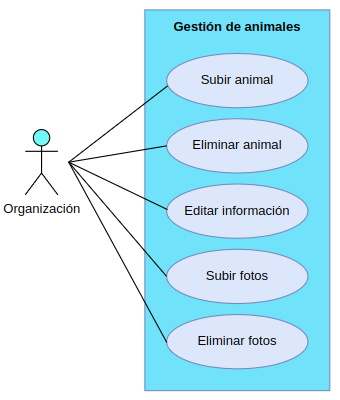
\includegraphics[width=0.8\textwidth]{imgs/gestion-animales}
    \caption{Gestión de animales}
    \label{fig:diagrama-caso-uso-gestion-animales}
\end{figure}

\subsubsection{Caso de Uso 2.1: Crear animal}\label{subsubsec:crear-animal}

\begin{table}[H]
    \begin{center}
        \begin{adjustbox}{width=\textwidth}
            \begin{tabular}{ | l | l | l | l | c | c | }
                \hline
                \textbf{Caso de uso} & \multicolumn{4}{l|}{Subir animal} & \cellcolor{gray!50} \textbf{CU-1.7}\\
                \hline
                \textbf{Actores} & \multicolumn{5}{p{0.5\linewidth}|}{Organización} \\
                \hline
                \textbf{Tipo} & \multicolumn{5}{l|}{Primario y esencial} \\
                \hline
                \textbf{Referencias} & \multicolumn{3}{l|}{RF-2.1} & \multicolumn{2}{l|}{ }\\
                \hline
                \textbf{Precondición} & \multicolumn{5}{l|}{La organización debe estar registrada previamente} \\
                \hline
                \textbf{Postcondición} & \multicolumn{5}{l|}{La organización sube un animal a la plataforma} \\
                \hline
                \textbf{Autor} & \multicolumn{1}{p{0.25\linewidth}|}{Manuel Ángel Rodríguez Segura} & \textbf{Fecha} &
                08-04-2023     & \textbf{Versión}                                                      & 1.0\\
                \hline
            \end{tabular}
        \end{adjustbox}
        \caption{CU-2.1: Subir animal}
        \label{tab:subir-animal}
    \end{center}
\end{table}

\begin{table}[H]
    \centering
    \begin{tabularx}{\textwidth}{@{} |L |@{}} \hline
        \rowcolor{gray!50}
        \textbf{Propósito} \\
        \hline
        Permite a una organización subir un animal a la plataforma. \\
        \hline
    \end{tabularx}
\end{table}

\begin{table}[H]
    \centering
    \begin{tabularx}{\textwidth}{@{} |L |@{}} \hline
        \rowcolor{gray!50}
        \textbf{Resumen} \\
        \hline
        Permite a una organización subir un animal a la aplicación para que pueda ser visto por los usuarios y adoptado
        por ellos. \\
        \hline
    \end{tabularx}
\end{table}

\subsubsection{Caso de Uso 2.2: Eliminar animal}\label{subsubsec:eliminar-animal}

\begin{table}[H]
    \begin{center}
        \begin{adjustbox}{width=\textwidth}
            \begin{tabular}{ | l | l | l | l | c | c | }
                \hline
                \textbf{Caso de uso} & \multicolumn{4}{l|}{Eliminar animal} & \cellcolor{gray!50} \textbf{CU-1.8}\\
                \hline
                \textbf{Actores} & \multicolumn{5}{p{0.5\linewidth}|}{Organización} \\
                \hline
                \textbf{Tipo} & \multicolumn{5}{l|}{Primario y esencial} \\
                \hline
                \textbf{Referencias} & \multicolumn{3}{l|}{RF-2.2} & \multicolumn{2}{l|}{ }\\
                \hline
                \textbf{Precondición} & \multicolumn{5}{l|}{El animal debe estar registrado en la plataforma previamente} \\
                \hline
                \textbf{Postcondición} & \multicolumn{5}{l|}{La organización elimina un animal de la plataforma} \\
                \hline
                \textbf{Autor} & \multicolumn{1}{p{0.25\linewidth}|}{Manuel Ángel Rodríguez Segura} & \textbf{Fecha} &
                08-04-2023     & \textbf{Versión}                                                      & 1.0\\
                \hline
            \end{tabular}
        \end{adjustbox}
        \caption{CU-2.2: Eliminar animal}
        \label{tab:eliminar-animal}
    \end{center}
\end{table}

\begin{table}[H]
    \centering
    \begin{tabularx}{\textwidth}{@{} |L |@{}} \hline
        \rowcolor{gray!50}
        \textbf{Propósito} \\
        \hline
        Permite a una organización eliminar un animal de la plataforma. \\
        \hline
    \end{tabularx}
\end{table}


\begin{table}[H]
    \centering
    \begin{tabularx}{\textwidth}{@{} |L |@{}} \hline
        \rowcolor{gray!50}
        \textbf{Resumen} \\
        \hline
        Permite a una organización eliminar un animal de la aplicación para que no pueda ser visto por los usuarios bien
    sea porque ya ha sido adoptado o porque no se desea que se vea. \\
        \hline
    \end{tabularx}
\end{table}

\subsubsection{Caso de Uso 2.3: Editar información}\label{subsubsec:editar-informacion-animal}

\begin{table}[H]
    \begin{center}
        \begin{adjustbox}{width=\textwidth}
            \begin{tabular}{ | l | l | l | l | c | c | }
                \hline
                \textbf{Caso de uso} & \multicolumn{4}{l|}{Editar información} & \cellcolor{gray!50} \textbf{CU-1.9}\\
                \hline
                \textbf{Actores} & \multicolumn{5}{p{0.5\linewidth}|}{Organización} \\
                \hline
                \textbf{Tipo} & \multicolumn{5}{l|}{Primario y esencial} \\
                \hline
                \textbf{Referencias} & \multicolumn{3}{l|}{RF-2.3} & \multicolumn{2}{l|}{ }\\
                \hline
                \textbf{Precondición} & \multicolumn{5}{l|}{El animal debe estar registrado en la plataforma previamente} \\
                \hline
                \textbf{Postcondición} & \multicolumn{5}{l|}{La organización edita la información de un animal de la plataforma} \\
                \hline
                \textbf{Autor} & \multicolumn{1}{p{0.25\linewidth}|}{Manuel Ángel Rodríguez Segura} & \textbf{Fecha} &
                08-04-2023     & \textbf{Versión}                                                      & 1.0\\
                \hline
            \end{tabular}
        \end{adjustbox}
        \caption{CU-2.3: Editar información}
        \label{tab:editar-animal}
    \end{center}
\end{table}

\begin{table}[H]
    \centering
    \begin{tabularx}{\textwidth}{@{} |L |@{}} \hline
        \rowcolor{gray!50}
        \textbf{Propósito} \\
        \hline
        Permite a una organización editar la información de un animal de la plataforma. \\
        \hline
    \end{tabularx}
\end{table}

\begin{table}[H]
    \centering
    \begin{tabularx}{\textwidth}{@{} |L |@{}} \hline
        \rowcolor{gray!50}
        \textbf{Resumen} \\
        \hline
        Permite a una organización editar la información de un animal de la aplicación para que los datos
    sean correctos y actualizados. \\
        \hline
    \end{tabularx}
\end{table}

\subsubsection{Caso de Uso 2.4: Subir fotos}\label{subsubsec:subir-fotos-animal}

\begin{table}[H]
    \begin{center}
        \begin{adjustbox}{width=\textwidth}
            \begin{tabular}{ | l | l | l | l | c | c | }
                \hline
                \textbf{Caso de uso} & \multicolumn{4}{l|}{Subir fotos} & \cellcolor{gray!50} \textbf{CU-1.10}\\
                \hline
                \textbf{Actores} & \multicolumn{5}{p{0.5\linewidth}|}{Organización} \\
                \hline
                \textbf{Tipo} & \multicolumn{5}{l|}{Primario y esencial} \\
                \hline
                \textbf{Referencias} & \multicolumn{3}{l|}{RF-2.4} & \multicolumn{2}{l|}{ }\\
                \hline
                \textbf{Precondición} & \multicolumn{5}{l|}{El animal debe estar registrado en la plataforma previamente} \\
                \hline
                \textbf{Postcondición} & \multicolumn{5}{l|}{La organización sube fotos de un animal de la plataforma} \\
                \hline
                \textbf{Autor} & \multicolumn{1}{p{0.25\linewidth}|}{Manuel Ángel Rodríguez Segura} & \textbf{Fecha} &
                08-04-2023     & \textbf{Versión}                                                      & 1.0\\
                \hline
            \end{tabular}
        \end{adjustbox}
        \caption{CU-2.4: Subir fotos}
        \label{tab:subir-fotos}
    \end{center}
\end{table}

\begin{table}[H]
    \centering
    \begin{tabularx}{\textwidth}{@{} |L |@{}} \hline
        \rowcolor{gray!50}
        \textbf{Propósito} \\
        \hline
        Permite a una organización subir fotos de un animal de la plataforma. \\
        \hline
    \end{tabularx}
\end{table}

\begin{table}[H]
    \centering
    \begin{tabularx}{\textwidth}{@{} |L |@{}} \hline
        \rowcolor{gray!50}
        \textbf{Resumen} \\
        \hline
        Permite a una organización subir fotos de un animal que esté registrado en la aplicación para que
    los usuarios puedan verlas. \\
        \hline
    \end{tabularx}
\end{table}

\subsubsection{Caso de Uso 2.5: Eliminar fotos}\label{subsubsec:eliminar-fotos-animal}

\begin{table}[H]
    \begin{center}
        \begin{adjustbox}{width=\textwidth}
            \begin{tabular}{ | l | l | l | l | c | c | }
                \hline
                \textbf{Caso de uso} & \multicolumn{4}{l|}{Eliminar fotos} & \cellcolor{gray!50} \textbf{CU-1.11}\\
                \hline
                \textbf{Actores} & \multicolumn{5}{p{0.5\linewidth}|}{Organización} \\
                \hline
                \textbf{Tipo} & \multicolumn{5}{l|}{Primario y esencial} \\
                \hline
                \textbf{Referencias} & \multicolumn{3}{l|}{RF-2.5} & \multicolumn{2}{l|}{ }\\
                \hline
                \textbf{Precondición} & \multicolumn{5}{l|}{El animal debe tener fotos subidas previamente} \\
                \hline
                \textbf{Postcondición} & \multicolumn{5}{l|}{La organización elimina fotos de un animal de la plataforma} \\
                \hline
                \textbf{Autor} & \multicolumn{1}{p{0.25\linewidth}|}{Manuel Ángel Rodríguez Segura} & \textbf{Fecha} &
                08-04-2023     & \textbf{Versión}                                                      & 1.0\\
                \hline
            \end{tabular}
        \end{adjustbox}
        \caption{CU-2.5: Eliminar fotos}
        \label{tab:eliminar-fotos}
    \end{center}
\end{table}

\begin{table}[H]
    \centering
    \begin{tabularx}{\textwidth}{@{} |L |@{}} \hline
        \rowcolor{gray!50}
        \textbf{Propósito} \\
        \hline
        Permite a una organización eliminar fotos de un animal de la plataforma. \\
        \hline
    \end{tabularx}
\end{table}

\begin{table}[H]
    \centering
    \begin{tabularx}{\textwidth}{@{} |L |@{}} \hline
        \rowcolor{gray!50}
        \textbf{Resumen} \\
        \hline
        Permite a una organización eliminar fotos de un animal que esté registrado en la aplicación para que las
    fotos estén actualizadas y con la información más reciente. \\
        \hline
    \end{tabularx}
\end{table}

\subsection{Gestión de peticiones}\label{subsec:gestion-de-peticiones}

\begin{figure}[H]
    \centering
    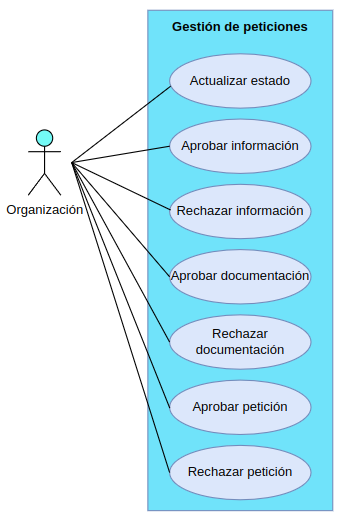
\includegraphics[width=0.8\textwidth]{imgs/gestion-peticiones}
    \caption{Gestión de peticiones}
    \label{fig:diagrama-caso-uso-gestion-peticiones}
\end{figure}

\subsubsection{Caso de Uso 3.1: Actualizar estado}\label{subsubsec:actualizar-estado-peticion}

\begin{table}[H]
    \begin{center}
        \begin{adjustbox}{width=\textwidth}
            \begin{tabular}{ | l | l | l | l | c | c | }
                \hline
                \textbf{Caso de uso} & \multicolumn{4}{l|}{Actualizar estado} & \cellcolor{gray!50} \textbf{CU-1.12}\\
                \hline
                \textbf{Actores} & \multicolumn{5}{p{0.5\linewidth}|}{Organización} \\
                \hline
                \textbf{Tipo} & \multicolumn{5}{l|}{Primario y esencial} \\
                \hline
                \textbf{Referencias} & \multicolumn{3}{l|}{RF-3.1} & \multicolumn{2}{l|}{ }\\
                \hline
                \textbf{Precondición} & \multicolumn{5}{l|}{La petición debe estar registrada en la plataforma previamente} \\
                \hline
                \textbf{Postcondición} & \multicolumn{5}{l|}{La organización actualiza el estado de una petición de la plataforma} \\
                \hline
                \textbf{Autor} & \multicolumn{1}{p{0.25\linewidth}|}{Manuel Ángel Rodríguez Segura} & \textbf{Fecha} &
                08-04-2023     & \textbf{Versión}                                                      & 1.0\\
                \hline
            \end{tabular}
        \end{adjustbox}
        \caption{CU-3.1: Actualizar estado}
        \label{tab:actualizar-estado}
    \end{center}
\end{table}

\begin{table}[H]
    \centering
    \begin{tabularx}{\textwidth}{@{} |L |@{}} \hline
        \rowcolor{gray!50}
        \textbf{Propósito} \\
        \hline
        Permite a una organización actualizar el estado de una petición de la plataforma. \\
        \hline
    \end{tabularx}
\end{table}

\begin{table}[H]
    \centering
    \begin{tabularx}{\textwidth}{@{} |L |@{}} \hline
        \rowcolor{gray!50}
        \textbf{Resumen} \\
        \hline
        Permite a una organización actualizar el estado de una petición que se haya realizado en la aplicación para
    que el usuario cuente con la información más reciente. \\
        \hline
    \end{tabularx}
\end{table}

\subsubsection{Caso de Uso 3.2: Eliminar petición}\label{subsubsec:eliminar-peticion}

\begin{table}[H]
    \begin{center}
        \begin{adjustbox}{width=\textwidth}
            \begin{tabular}{ | l | l | l | l | c | c | }
                \hline
                \textbf{Caso de uso} & \multicolumn{4}{l|}{Aprobar información} & \cellcolor{gray!50} \textbf{CU-1.13}\\
                \hline
                \textbf{Actores} & \multicolumn{5}{p{0.5\linewidth}|}{Organización} \\
                \hline
                \textbf{Tipo} & \multicolumn{5}{l|}{Primario y esencial} \\
                \hline
                \textbf{Referencias} & \multicolumn{3}{l|}{RF-3.2} & \multicolumn{2}{l|}{ }\\
                \hline
                \textbf{Precondición} & \multicolumn{5}{l|}{La petición debe estar registrada en la plataforma previamente
                y la información no puede estar rechazada} \\
                \hline
                \textbf{Postcondición} & \multicolumn{5}{l|}{La organización aprueba la información de una petición de la plataforma} \\
                \hline
                \textbf{Autor} & \multicolumn{1}{p{0.25\linewidth}|}{Manuel Ángel Rodríguez Segura} & \textbf{Fecha} &
                08-04-2023     & \textbf{Versión}                                                      & 1.0\\
                \hline
            \end{tabular}
        \end{adjustbox}
        \caption{CU-3.2: Aprobar información}
        \label{tab:aprobar-informacion}
    \end{center}
\end{table}

\newpage

\begin{table}[H]
    \centering
    \begin{tabularx}{\textwidth}{@{} |L |@{}} \hline
        \rowcolor{gray!50}
        \textbf{Propósito} \\
        \hline
        Permite a una organización aprobar la información de una petición de la plataforma. \\
        \hline
    \end{tabularx}
\end{table}

\begin{table}[H]
    \centering
    \begin{tabularx}{\textwidth}{@{} |L |@{}} \hline
        \rowcolor{gray!50}
        \textbf{Resumen} \\
        \hline
        Permite a una organización aprobar la información que ha proporcionado un usuario en una petición que se haya
    realizado en la aplicación previamente. \\
        \hline
    \end{tabularx}
\end{table}

\subsubsection{Caso de Uso 3.3: Rechazar información}\label{subsubsec:rechazar-informacion}

\begin{table}[H]
    \begin{center}
        \begin{adjustbox}{width=\textwidth}
            \begin{tabular}{ | l | l | l | l | c | c | }
                \hline
                \textbf{Caso de uso} & \multicolumn{4}{l|}{Rechazar información} & \cellcolor{gray!50} \textbf{CU-1.14}\\
                \hline
                \textbf{Actores} & \multicolumn{5}{p{0.5\linewidth}|}{Organización} \\
                \hline
                \textbf{Tipo} & \multicolumn{5}{l|}{Primario y esencial} \\
                \hline
                \textbf{Referencias} & \multicolumn{3}{l|}{RF-3.3} & \multicolumn{2}{l|}{ }\\
                \hline
                \textbf{Precondición} & \multicolumn{5}{l|}{La petición debe estar registrada en la plataforma previamente y
                la información no puede estar aprobada} \\
                \hline
                \textbf{Postcondición} & \multicolumn{5}{l|}{La organización rechaza la información de una petición de la plataforma} \\
                \hline
                \textbf{Autor} & \multicolumn{1}{p{0.25\linewidth}|}{Manuel Ángel Rodríguez Segura} & \textbf{Fecha} &
                08-04-2023     & \textbf{Versión}                                                      & 1.0\\
                \hline
            \end{tabular}
        \end{adjustbox}
        \caption{CU-3.3: Rechazar información}
        \label{tab:rechazar-informacion}
    \end{center}
\end{table}

\begin{table}[H]
    \centering
    \begin{tabularx}{\textwidth}{@{} |L |@{}} \hline
        \rowcolor{gray!50}
        \textbf{Propósito} \\
        \hline
        Permite a una organización rechazar la información de una petición de la plataforma. \\
        \hline
    \end{tabularx}
\end{table}

\begin{table}[H]
    \centering
    \begin{tabularx}{\textwidth}{@{} |L |@{}} \hline
        \rowcolor{gray!50}
        \textbf{Resumen} \\
        \hline
        Permite a una organización rechazar la información que ha proporcionado un usuario en una petición que se haya
    realizado en la aplicación previamente. \\
        \hline
    \end{tabularx}
\end{table}

\newpage

\subsubsection{Caso de Uso 3.4: Aprobar documentación}\label{subsubsec:aprobar-documentacion}

\begin{table}[H]
    \begin{center}
        \begin{adjustbox}{width=\textwidth}
            \begin{tabular}{ | l | l | l | l | c | c | }
                \hline
                \textbf{Caso de uso} & \multicolumn{4}{l|}{Aprobar documentación} & \cellcolor{gray!50} \textbf{CU-1.15}\\
                \hline
                \textbf{Actores} & \multicolumn{5}{p{0.5\linewidth}|}{Organización} \\
                \hline
                \textbf{Tipo} & \multicolumn{5}{l|}{Primario y esencial} \\
                \hline
                \textbf{Referencias} & \multicolumn{3}{l|}{RF-3.4} & \multicolumn{2}{l|}{ }\\
                \hline
                \textbf{Precondición} & \multicolumn{5}{l|}{La petición debe estar registrada en la aplicación,
                el usuario debe haber enviado la documentación previamente y no puede estar rechazada} \\
                \hline
                \textbf{Postcondición} & \multicolumn{5}{l|}{La organización aprueba la documentación de una petición de la plataforma} \\
                \hline
                \textbf{Autor} & \multicolumn{1}{p{0.25\linewidth}|}{Manuel Ángel Rodríguez Segura} & \textbf{Fecha} &
                08-04-2023     & \textbf{Versión}                                                      & 1.0\\
                \hline
            \end{tabular}
        \end{adjustbox}
        \caption{CU-3.4: Aprobar documentación}
        \label{tab:aprobar-documentacion}
    \end{center}
\end{table}

\begin{table}[H]
    \centering
    \begin{tabularx}{\textwidth}{@{} |L |@{}} \hline
        \rowcolor{gray!50}
        \textbf{Propósito} \\
        \hline
        Permite a una organización aprobar la documentación que ha enviado un usuario en una petición. \\
        \hline
    \end{tabularx}
\end{table}

\begin{table}[H]
    \centering
    \begin{tabularx}{\textwidth}{@{} |L |@{}} \hline
        \rowcolor{gray!50}
        \textbf{Resumen} \\
        \hline
        Permite a una organización aprobar la documentación que ha proporcionado un usuario en una petición que se haya
    realizado en la aplicación previamente. \\
        \hline
    \end{tabularx}
\end{table}

\subsubsection{Caso de Uso 3.5: Rechazar documentación}\label{subsubsec:rechazar-documentacion}

\begin{table}[H]
    \begin{center}
        \begin{adjustbox}{width=\textwidth}
            \begin{tabular}{ | l | l | l | l | c | c | }
                \hline
                \textbf{Caso de uso} & \multicolumn{4}{l|}{Rechazar documentación} & \cellcolor{gray!50} \textbf{CU-1.16}\\
                \hline
                \textbf{Actores} & \multicolumn{5}{p{0.5\linewidth}|}{Organización} \\
                \hline
                \textbf{Tipo} & \multicolumn{5}{l|}{Primario y esencial} \\
                \hline
                \textbf{Referencias} & \multicolumn{3}{l|}{RF-3.5} & \multicolumn{2}{l|}{ }\\
                \hline
                \textbf{Precondición} & \multicolumn{5}{l|}{La petición debe estar registrada en la aplicación,
                el usuario debe haber enviado la documentación previamente y no puede estar aprobada.} \\
                \hline
                \textbf{Postcondición} & \multicolumn{5}{l|}{La organización rechaza la documentación de una petición de la plataforma} \\
                \hline
                \textbf{Autor} & \multicolumn{1}{p{0.25\linewidth}|}{Manuel Ángel Rodríguez Segura} & \textbf{Fecha} &
                08-04-2023     & \textbf{Versión}                                                      & 1.0\\
                \hline
            \end{tabular}
        \end{adjustbox}
        \caption{CU-3.5: Rechazar documentación}
        \label{tab:rechazar-documentacion}
    \end{center}
\end{table}

\begin{table}[H]
    \centering
    \begin{tabularx}{\textwidth}{@{} |L |@{}} \hline
        \rowcolor{gray!50}
        \textbf{Propósito} \\
        \hline
        Permite a una organización rechazar la documentación que ha enviado un usuario en una petición. \\
        \hline
    \end{tabularx}
\end{table}

\begin{table}[H]
    \centering
    \begin{tabularx}{\textwidth}{@{} |L |@{}} \hline
        \rowcolor{gray!50}
        \textbf{Resumen} \\
        \hline
        Permite a una organización rechazar la documentación que ha proporcionado un usuario en una petición que se haya
    realizado en la aplicación previamente. \\
        \hline
    \end{tabularx}
\end{table}

\subsubsection{Caso de Uso 3.6: Aprobar petición}\label{subsubsec:aprobar-peticion}

\begin{table}[H]
    \begin{center}
        \begin{adjustbox}{width=\textwidth}
            \begin{tabular}{ | l | l | l | l | c | c | }
                \hline
                \textbf{Caso de uso} & \multicolumn{4}{l|}{Aprobar petición} & \cellcolor{gray!50} \textbf{CU-1.17}\\
                \hline
                \textbf{Actores} & \multicolumn{5}{p{0.5\linewidth}|}{Organización} \\
                \hline
                \textbf{Tipo} & \multicolumn{5}{l|}{Primario y esencial} \\
                \hline
                \textbf{Referencias} & \multicolumn{3}{l|}{RF-3.6} & \multicolumn{2}{l|}{ }\\
                \hline
                \textbf{Precondición} & \multicolumn{5}{l|}{La petición debe estar registrada en la aplicación y
                la información y documentación del usuario deben estar aprobadas previamente} \\
                \hline
                \textbf{Postcondición} & \multicolumn{5}{l|}{La organización aprueba la petición de la plataforma} \\
                \hline
                \textbf{Autor} & \multicolumn{1}{p{0.25\linewidth}|}{Manuel Ángel Rodríguez Segura} & \textbf{Fecha} &
                08-04-2023     & \textbf{Versión}                                                      & 1.0\\
                \hline
            \end{tabular}
        \end{adjustbox}
        \caption{CU-3.6: Aprobar petición}
        \label{tab:aprobar-peticion}
    \end{center}
\end{table}

\begin{table}[H]
    \centering
    \begin{tabularx}{\textwidth}{@{} |L |@{}} \hline
        \rowcolor{gray!50}
        \textbf{Propósito} \\
        \hline
        Permite a una organización aprobar una petición. \\
        \hline
    \end{tabularx}
\end{table}

\begin{table}[H]
    \centering
    \begin{tabularx}{\textwidth}{@{} |L |@{}} \hline
        \rowcolor{gray!50}
        \textbf{Resumen} \\
        \hline
        Permite a una organización aprobar una petición que se haya realizado en la aplicación previamente. \\
        \hline
    \end{tabularx}
\end{table}

\subsubsection{Caso de Uso 3.7: Rechazar petición}\label{subsubsec:rechazar-peticion}

\begin{table}[H]
    \begin{center}
        \begin{adjustbox}{width=\textwidth}
            \begin{tabular}{ | l | l | l | l | c | c | }
                \hline
                \textbf{Caso de uso} & \multicolumn{4}{l|}{Rechazar petición} & \cellcolor{gray!50} \textbf{CU-1.18}\\
                \hline
                \textbf{Actores} & \multicolumn{5}{p{0.5\linewidth}|}{Organización} \\
                \hline
                \textbf{Tipo} & \multicolumn{5}{l|}{Primario y esencial} \\
                \hline
                \textbf{Referencias} & \multicolumn{3}{l|}{RF-3.7} & \multicolumn{2}{l|}{ }\\
                \hline
                \textbf{Precondición} & \multicolumn{5}{l|}{La petición debe estar registrada en la aplicación previamente} \\
                \hline
                \textbf{Postcondición} & \multicolumn{5}{l|}{La organización rechaza la petición de la plataforma} \\
                \hline
                \textbf{Autor} & \multicolumn{1}{p{0.25\linewidth}|}{Manuel Ángel Rodríguez Segura} & \textbf{Fecha} &
                08-04-2023     & \textbf{Versión}                                                      & 1.0\\
                \hline
            \end{tabular}
        \end{adjustbox}
        \caption{CU-3.7: Rechazar petición}
        \label{tab:rechazar-peticion}
    \end{center}
\end{table}

\begin{table}[H]
    \centering
    \begin{tabularx}{\textwidth}{@{} |L |@{}} \hline
        \rowcolor{gray!50}
        \textbf{Propósito} \\
        \hline
        Permite a una organización rechazar una petición. \\
        \hline
    \end{tabularx}
\end{table}

\begin{table}[H]
    \centering
    \begin{tabularx}{\textwidth}{@{} |L |@{}} \hline
        \rowcolor{gray!50}
        \textbf{Resumen} \\
        \hline
        Permite a una organización rechazar una petición que se haya realizado en la aplicación previamente. \\
        \hline
    \end{tabularx}
\end{table}

Para entender de forma gráfica cómo funciona el flujo de una petición de adopción desde que se crea por el usuario hasta que se acepta
por parte de la organización, se puede consultar la siguiente figura: \\

\begin{figure}[H]
    \centering
    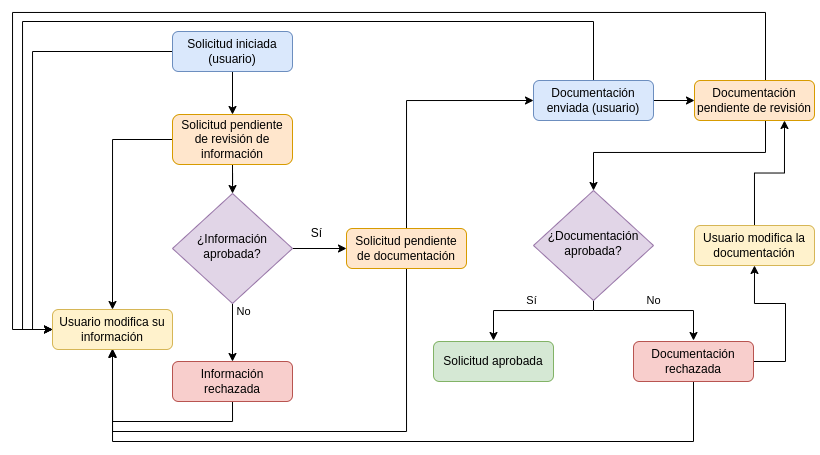
\includegraphics[width=1.0\textwidth]{imgs/estados-peticion.png}
    \caption{Flujo de una petición de adopción}
    \label{fig:flujo-peticion}
\end{figure}

    \chapter{Arquitectura y diseño}\label{ch:arquitectura-y-diseno}

En este capítulo se detallan los aspectos de diseño y arquitectura del proyecto. Para la realización de este proyecto
se han utilizado diferentes herramientas y tecnologías que se detallan en los siguientes apartados.

\section{Arquitectura}\label{sec:arquitectura}

De forma visual, la arquitectura de todo el proyecto se puede contemplar en la siguiente imagen:

\begin{figure}[H]
    \centering
    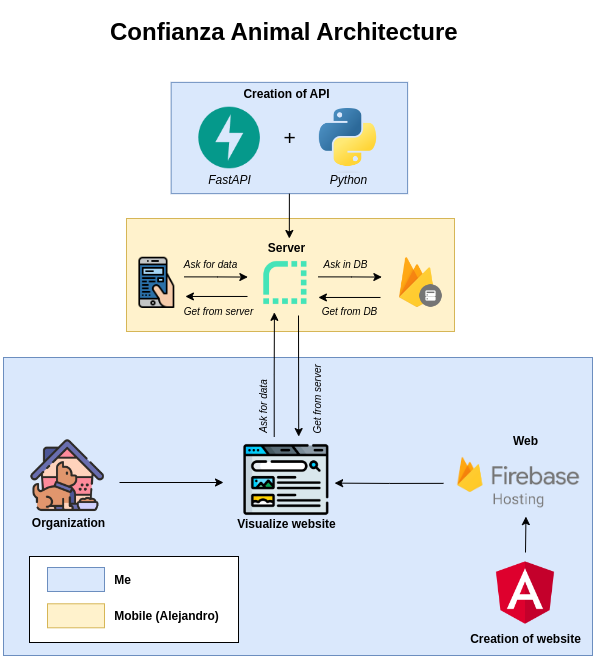
\includegraphics[width=1\textwidth]{imgs/arquitectura2.png}
    \caption{Arquitectura del proyecto}
    \label{fig:arquitectura}
\end{figure}

A primera vista, vemos que el diagrama de la arquitectura se trata de un modelo
\textbf{cliente/servidor} en el que tanto el usuario mobile (parte amarilla que referencia la arquitectura de mi compañero Alejandro)
como las organizaciones, se comunican con el servidor por medio de una \textbf{API}. En concreto,
la arquitectura consta de los siguientes elementos:

\newpage

\begin{itemize}
    \item \textbf{Cliente}: se trata de la página web que se comunica con la \textbf{API} para obtener los datos de la aplicación.
    \item \textbf{Servidor}: se trata de la \textbf{API} que se comunica con los servicios y la base de datos de Firebase.
    \item \textbf{Base de datos}: se trata de la base de datos en la nube de Firebase que almacena los datos de la aplicación.
    \item \textbf{Servicios}: se trata de los servicios de Firebase que se utilizan para la autenticación, el almacenamiento
    de archivos, el envío de notificaciones, etc.
\end{itemize}

El hecho de escoger esta arquitectura se debe a que es la más utilizada en la actualidad para el desarrollo de aplicaciones
web y móviles y ofrece una mayor serie de ventajas con respecto a otras alternativas como puede ser la arquitectura \textbf{peer-to-peer}
en la que los clientes se comunican entre sí sin necesidad de un servidor. Para realizar la comunicación entre el cliente
y el servidor se utiliza el protocolo HTTP. Por medio de este protocolo el cliente y el servidor pueden
intercambiar información por medio de peticiones y respuestas HTTP. \\

Al ser HTTP un protocolo sin estado, es decir, que no mantiene la información de las peticiones anteriores, permite
manejar las peticiones de forma concurrente y así mejorar el rendimiento y la escalabilidad de la aplicación. Estos
motivos hacen que su uso se haya extendido a la mayoría de las aplicaciones web y móviles. \\

Además, este tipo de arquitectura permite separar la lógica de negocio de la aplicación del cliente y alojarla en el
servidor. Esto permite que el cliente no tenga acceso a la información sensible de la aplicación y que la lógica de
negocio pueda ser reutilizada en otros clientes. También permite que el cliente pueda autenticarse para acceder a la
información del servidor y que no tenga que realizar ninguna operación de procesamiento de datos dando lugar a una
aplicación más rápida y con mejor rendimiento.

\newpage

\section{Diseño}\label{sec:diseno}

Para llevar a cabo el diseño de la aplicación se van a utilizar una serie de herramientas y tecnologías de las cuales
se ha justificado su elección en el apartado~\ref{sec:eleccion-de-herramientas-y-tecnologias}. Vamos a ver en detalle
cómo se ha planteado el diseño para la página web, la \textbf{API} y la base de datos:

\begin{enumerate}
    \item \textbf{Diseño de la página web}:
    \begin{itemize}
        \item En base a los requisitos del sistema, se definen los componentes y servicios que se van a utilizar en la
        aplicación.
        \item Para establecer las rutas de la aplicación se utiliza el enrutador de Angular.
        \item Para la comunicación con la \textbf{API} se utilizan los servicios creados y un servicio propio de Angular llamado
        \textbf{HttpClient} que permite realizar peticiones HTTP al servidor.
    \end{itemize}
    \item \textbf{Diseño de la API}:
    \begin{itemize}
        \item En base a los requisitos del sistema, se definen los endpoints que se van a utilizar en la \textbf{API}.
        \item Se definen los modelos de datos que se van a utilizar en la \textbf{API}.
        \item Se implementan los \textit{endpoints} que van a ser utilizados por la aplicación y que van
        a interactuar con la base de datos.
    \end{itemize}
    \item \textbf{Diseño de la base de datos}:
    \begin{itemize}
        \item En base a los requisitos del sistema, se definen las colecciones y estructuras de datos que se van a utilizar
        en la base de datos.
        \item Se definen las reglas de seguridad de la base de datos para que los datos estén protegidos e impedir
        accesos no autorizados.
    \end{itemize}
\end{enumerate}

Todos los detalles de implementación y despliegues que han permitido llevar a cabo la arquitectura y diseño de la aplicación se
detallan en el capítulo:~\ref{ch:implementacion-y-despliegues}.

\newpage

\section{Patrones de diseño}\label{subsec:patrones-de-diseno}

Una vez definida la arquitectura y el diseño de la aplicación, se han implementado una serie de patrones de diseño que
han ayudado a solucionar los problemas. Un patrón de diseño es una solución general y reutilizable a un problema que
ocurre con frecuencia dentro de un contexto dado en el diseño de software. Son una serie de buenas prácticas que se
pueden aplicar a cualquier proyecto de software y que permiten resolver problemas de forma más eficiente. \\

En este proyecto se han utilizado los siguientes patrones de diseño:

\begin{itemize}
    \item \textbf{Inyección de dependencias}: Se trata de un patrón de diseño que consiste en insertar las dependencias
    de un objeto en el momento de su creación. Esto permite que el objeto sea independiente de las dependencias que
    necesita para funcionar y que pueda ser reutilizado en cualquiera otra parte del código sin necesidad de crear
    una nueva instancia. Este patrón se ha utilizado para inyectar los servicios que se utilizan
    en los componentes de Angular.

    \item \textbf{Observable}: Es un patrón de diseño que permite la comunicación entre objetos de forma reactiva.
    Esto significa que cuando un objeto emite un evento, los objetos que están suscritos a ese evento son notificados
    y pueden realizar una acción. Este patrón se ha utilizado para comunicar los componentes de la web con
    los servicios y viceversa.

    \newpage

    \item \textbf{Redux}: Por medio de la librería \textbf{NgRx} se ha implementado el patrón de diseño \textbf{Redux} en la
    página web. Este patrón de diseño se basa en el concepto de \textbf{almacén centralizado} en el que se almacenan
    los datos de la aplicación. Los componentes de Angular se suscriben a los datos del almacén y cuando estos cambian
    se actualizan automáticamente. Este patrón de diseño permite que la aplicación sea escalable y que los datos
    se puedan compartir entre diferentes componentes de forma sencilla y muy rápida:
        \begin{figure}[H]
            \centering
            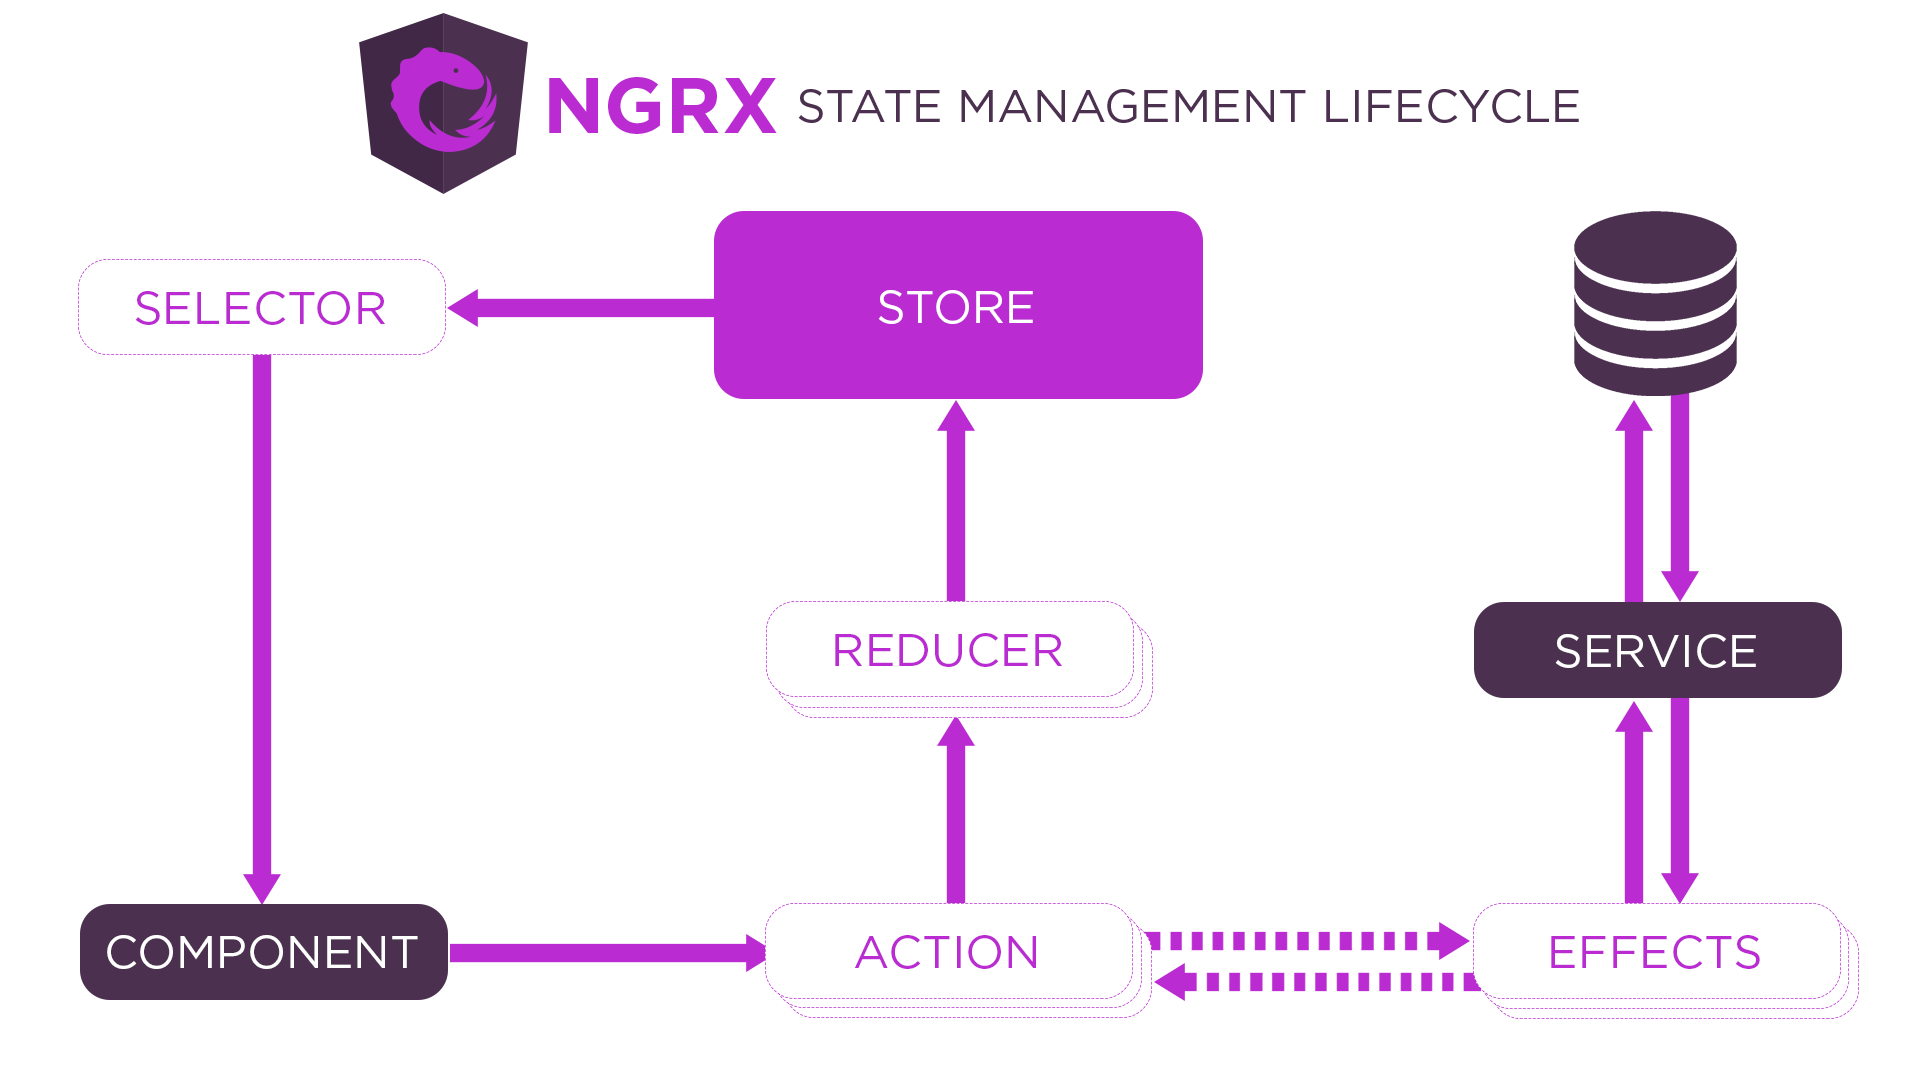
\includegraphics[width=0.9\textwidth]{imgs/ngrx.png}
            \caption{Patrón Redux con NgRx. Fuente~\cite{ngrx}}
            \label{fig:redux}
        \end{figure}
    \item \textbf{Factory method}: Este patrón de diseño se utiliza para crear objetos de una misma clase de forma
    sencilla y rápida y encapsular la lógica de creación de los objetos.

    \newpage

    \item \textbf{MVC}: Este patrón de diseño divide la aplicación en tres capas: modelo, vista y
    controlador (MVC). El modelo representa la lógica de negocio de la aplicación, la vista es la interfaz de usuario
    y el controlador es el encargado de gestionar las peticiones del usuario y comunicar los datos del modelo con la vista.
    La mejor forma de conocer el funcionamiento de este patrón de diseño es a través de una imagen explicativa:
        \begin{figure}[H]
            \centering
            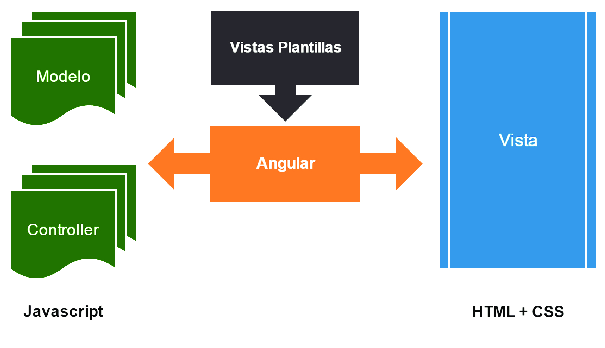
\includegraphics[width=0.9\textwidth]{imgs/mvc.png}
            \caption{Patrón MVC. Fuente~\cite{mvc}}
            \label{fig:mvc}
        \end{figure}
    \item \textbf{Composite}: Este patrón de diseño se utiliza para crear estructuras jerárquicas de objetos. En este
    proyecto se ha utilizado para crear la estructura jerárquica de los diferentes tipos de animales que se pueden
    englobar en una categoría denominada \textit{Animal}.
\end{itemize}

    \chapter{Implementación y despliegues}\label{ch:implementacion-y-despliegues}

En este capítulo se profundiza en los detalles de la implementación de la página web y la API a lo largo de los diferentes
\textit{sprints} que se han realizado durante el desarrollo del proyecto. Además, se explican los detalles de los despliegues
de la página web y la API así como las herramientas y tecnologías que se han utilizado para llevarlos a cabo.

\section{Desarrollo basado en sprints}\label{sec:desarrollo-basado-en-sprints}

Tal y como se ha mencionado en la subsección:~\ref{subsec:metodologia}, el desarrollo del proyecto se ha
realizado siguiendo una metodología ágil basada en \textit{sprints}. En este caso, se han ido completando los diferentes hitos del proyecto a lo largo de los
\textit{sprints} en los que se han incluidos tareas más específicas que permiten que el desarrollo sea más rápido y
eficiente.

\subsection{Sprints 1-4}\label{subsec:sprints-1-4}

En los cuatro primeros \textit{sprints} se han llevado a cabo las tareas que han permitido preparar los entornos de desarrollo
para la creación de la página web y la API. En concreto, se han llevado a cabo las siguientes tareas:

\begin{itemize}
    \item Creación de los repositorios de la página web y la API.
    \item Creación de la estructura de los proyectos y de la base de datos.
    \item Creación de la estructura inicial de la documentación del proyecto en \textit{LaTeX}.
    \item Fijación de objetivos y alcance del proyecto.
    \item Fijación de la metodología de desarrollo y requisitos del proyecto.
    \item Arquitectura del proyecto.
    \item Diseño de la API, página web y base de datos.
\end{itemize}

\subsubsection{Creación de la API}\label{subsubsec:creacion-de-la-api}

Para la creación de la API se ha usado el framework \textit{FastAPI} por medio del lenguaje de programación \textit{Python} el cual
se ha explicado en profundidad en la subsección:~\ref{subsec:framework-web-de-api}. Todo el código de la API se ha desarrollado
siguiendo la documentación oficial de \textit{FastAPI} que se puede consultar en la siguiente dirección: \url{https://fastapi.tiangolo.com/} y
las buenas prácticas de desarrollo de APIs que se pueden consultar en la siguiente dirección: \url{https://docs.microsoft.com/en-us/azure/architecture/best-practices/api-design}.
A continuación se van a mostrar los pasos que se han seguido en concreto para la creación de la API del proyecto:

\begin{enumerate}
    \item Instalar \textit{FastAPI} y \textit{uvicorn} por medio de \textit{pip} con el comando
    \textit{pip install fastapi uvicorn}.
    \item Crear un fichero \textit{main.py} que contendrá el código de la API que se ejecutará con el comando
    \textit{uvicorn main:app --reload}. El parámetro \textit{--reload} permite que cada vez que se realice un cambio
    en el código, el servidor se reinicie automáticamente.
    \item Definir las clases y esquemas de datos que se van a utilizar en la API.
    \item Definir las rutas que tendrá la API. En este proyecto se han definido las siguientes:
        \begin{itemize}
            \item \textbf{/auth}: ruta para reestablecer la contraseña de un usuario u organización
            \item \textbf{/organizations}: ruta que engloba todos los endpoints relacionados con las organizaciones
            \item \textbf{/users}: ruta que engloba todos los endpoints relacionados con los usuarios
            \item \textbf{/animals}: ruta que engloba todos los endpoints relacionados con los animales
            \item \textbf{/petitions}: ruta que engloba todos los endpoints relacionados con las peticiones
            \item \textbf{/filters}: ruta que engloba todos los endpoints relacionados con los filtros de búsqueda
        \end{itemize}
    \item Implementar los diferentes \textit{endpoints} dentro de cada ruta.
    \item Crear los tests para cada uno de los \textit{endpoints} de la API. Estos tests se pueden consultar en la
    subsección de testing:~\ref{subsubsec:tests}.
\end{enumerate}

\subsubsection{Clases}\label{subsubsec:clases}

Antes de iniciar con la implementación de los \textit{endpoints} de la API es necesario definir las clases y esquemas de datos
que se van a utilizar. En la siguiente imagen se puede ver de forma esquemática las clases que se han definido para el proyecto:

\begin{figure}[H]
    \centering
    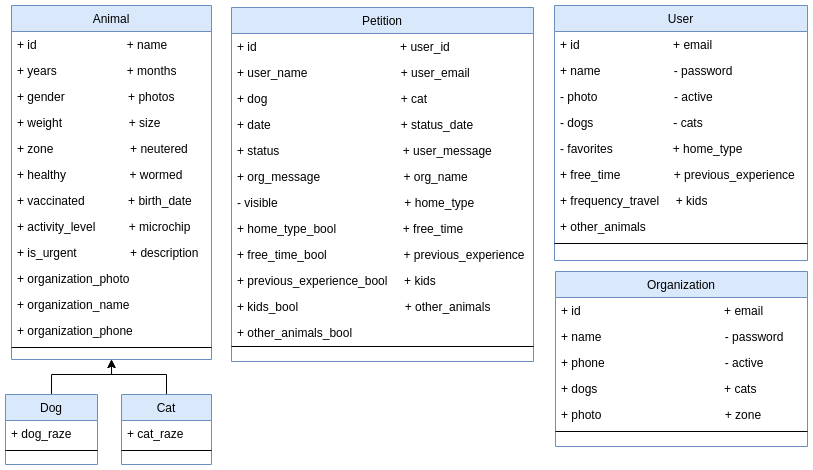
\includegraphics[width=0.9\textwidth]{imgs/clases.png}
    \caption{Clases}
    \label{fig:clases}
\end{figure}

Como vemos se han definido las siguientes clases:

\begin{itemize}
    \item \textbf{Animal}: con sus respectivos atributos (id, años, nombre, fotos, etc.)
    \item \textbf{Dog}: que hereda de la clase \textit{Animal} y que añade su propio atributo (raza)
    \item \textbf{Cat}: que hereda de la clase \textit{Animal} y que añade su propio atributo (raza)
    \item \textbf{Petition}: con sus respectivos atributos (id, fecha, estado, etc.)
    \item \textbf{User}: con sus respectivos atributos (id, nombre, foto, etc.)
    \item \textbf{Organization}: con sus respectivos atributos (id, nombre, email, foto, etc.)
\end{itemize}

Además se ha diferenciado si el atributo es de consulta \textbf{privado} por medio del símbolo \textit{-} o de consulta
\textbf{público} por medio del símbolo \textit{+}. Por ejemplo, el atributo \textit{email} de la clase \textit{Organization}
es público porque se puede consultar por medio de la API, mientras que el atributo \textit{password} de la clase
\textit{User} es privado ya que no sería recomendable que se pudiera acceder a él por medio de una consulta.

\subsubsection{Códigos de estado de respuesta HTTP}\label{subsubsec:codigos-de-error}

A la hora de implementar una API, es importante tener en cuenta los códigos de estado que se pueden devolver en cada petición HTTP. En este caso, se ha
seguido la especificación de \href{https://developer.mozilla.org/es/docs/Web/HTTP/Status}{MDN Web Docs} para devolver los códigos más
adecuados en cada caso. A continuación, se muestra una tabla con los diferentes códigos que se han utilizado a lo largo del desarrollo:

\begin{table}[H]
    \centering
    \begin{tabular}{|c|c|}
        \hline
        \textbf{Código de error} & \textbf{Descripción} \\
        \hline
        200 & OK \\
        \hline
        204 & Sin contenido \\
        \hline
        400 & Petición incorrecta \\
        \hline
        401 & No autorizado \\
        \hline
        403 & Prohibido \\
        \hline
        404 & No encontrado \\
        \hline
        500 & Error interno del servidor \\
        \hline
    \end{tabular}
    \caption{Códigos de respuesta HTTP}
    \label{tab:codigos-respuesta-http}
\end{table}

Un ejemplo de ello podría ser la petición de adopción de una mascota. Si el usuario no está autenticado en el sistema, se devolvería un código de error
401 (no autorizado). Si el usuario está autenticado, pero no se ha encontrado la mascota que se quiere adoptar, se devolvería un código de error 404 (no encontrado).
Si la petición se ha realizado correctamente, se devolvería un código de estado 200 (OK). \\

Los códigos de error 500 (error interno del servidor) y 400 (petición incorrecta) se han utilizado en casos en los que se ha producido un error en el servidor
o en el cliente, respectivamente. Por ejemplo, si se ha producido un error al realizar una consulta a la base de datos, se devolvería un código de error 500.
Si el usuario ha enviado una petición con un formato incorrecto, se devolvería un código de error 400.

\subsubsection{Creación de la página web}\label{subsubsec:creacion-de-la-pagina-web}

La estructura del proyecto en Angular se basa en componentes, servicios y módulos (patrón módulo). Los módulos se utilizan
para organizar y estructurar la aplicación en diferentes partes así como separar la lógica en diferentes ficheros. Cada módulo
se compone de componentes y servicios. Los componentes se encargan de la parte visual de la aplicación y los servicios
se encargan de la lógica de la aplicación. El proyecto de la página web se compone de los siguientes elementos:

\begin{itemize}
    \item \textbf{Directorio \textit{src}:} directorio principal de la aplicación. En este directorio se encuentran los ficheros
    de configuración de la aplicación, los ficheros de \textit{testing} y los ficheros de la aplicación. También se encuentran
    los componentes, servicios, directivas y el resto de elementos.
    \item \textbf{Directorio \textit{app}:} este directorio contiene el componente principal de la aplicación, el componente \textit{app.component}.
    Este es el componente que se carga al iniciar la aplicación y que a su vez contiene la llamada al resto de componentes.
    \item \textbf{Directorio \textit{assets}:} este directorio contiene los recursos de la aplicación como imágenes, iconos, etc.
    \item \textbf{Directorio \textit{environments}:} este directorio contiene los ficheros de configuración de los entornos de la aplicación (producción y desarrollo).
    \item \textbf{Directorio \textit{services}:} este directorio contiene los diferentes servicios de la aplicación que se encargan a su vez de realizar
    las peticiones a la API.
    \item \textbf{Directorio \textit{components}:} este directorio contiene los diferentes componentes de la aplicación. Cada componente se compone de un fichero
    \textit{.ts} que contiene la lógica del componente, un fichero \textit{.html} que contiene la parte visual del componente, un fichero \textit{.scss}
    que contiene los estilos del componente y un fichero \textit{.spec.ts} que contiene los tests del componente.
    \item \textbf{Directorio \textit{interfaces}:} este directorio contiene las interfaces de la aplicación. Estas interfaces se utilizan para definir
    los tipos de datos que se van a utilizar en la aplicación.
    \item \textbf{Archivo \textit{index.html}:} este archivo contiene la estructura básica de la página web. Aquí se vinculan los diferentes ficheros de estilos
    y scripts necesarios para el correcto funcionamiento de la aplicación.
\end{itemize}

Esta estructura ofrece numerosas ventajas frente a otros \textit{frameworks} como puede ser la \textbf{modularidad} de la aplicación. De esta forma,
la aplicación se convierte más fácil de mantener y de escalar. Otra de las ventajas es la \textbf{reutilización} de componentes. De esta forma, si
se quiere utilizar un componente en diferentes partes de la aplicación, solo es necesario importarlo en el componente que se desee. También
ofrece la ventaja de la \textbf{separación de responsabilidades}. Existen servicios, componentes, directivas y otros elementos
que de forma individual se encargan de una tarea concreta.

\subsubsection{Creación de Bases de Datos}\label{subsec:creacion-de-bases-de-datos}

Para el proyecto se han creados dos bases de datos: una para la versión de desarrollo y otra para la versión de producción.
Ambas, por medio de \textbf{Firebase} cuentan con la misma estructura y se encuentran en la nube, pero la base de datos de
producción cuenta con una serie de reglas que limitan el acceso a la misma y que se detallan en la subsección:~\ref{subsubsec:reglas} a
diferencia de la base de datos de desarrollo que no cuenta con ese tipo de restricciones y que se ha usado exclusivamente para
probar la funcionalidad de la API. \\

Las bases de datos de Firebase son bases de datos no relacionales que se basan en colecciones que pueden contener un número ilimitado de documentos.
Cada documento a su vez se compone de una serie de campos que pueden ser de diferentes tipos (texto, número, booleano, etc.).
Vamos a desgranar cada uno de estos conceptos en las siguientes subsecciones.

\newpage

\subsubsection{Colecciones}\label{subsubsec:colecciones}

Las colecciones son el elemento principal de las bases de datos de Firebase. Cada colección puede contener un número ilimitado de documentos
y cada documento puede contener un número ilimitado de campos. Podemos ver las colecciones como las tablas de una base de datos relacional
y los documentos como las filas de dichas tablas. \\

En este proyecto se han creado las siguientes colecciones:

\begin{itemize}
    \item \textbf{Animals}: Colección que contiene un documento \textit{animals} que a su vez contiene todos los animales que se encuentran en la base de datos.
    \item \textbf{Users}: Colección que contiene un documento con el \textit{id} de cada usuario que se ha registrado en la aplicación y que a su vez contiene
    todos los datos de dicho usuario.
    \item \textbf{Organization}: Colección que contiene un documento con el \textit{id} de cada organización que se ha registrado en la aplicación y que a su vez contiene
    todos los datos de dicha organización.
    \item \textbf{Petitions}: Colección que contiene un documento con el \textit{id} de cada petición que se ha realizado en la aplicación y que a su vez contiene
    todos los datos de dicha petición.
\end{itemize}

En la siguiente figura se puede ver un ejemplo de la estructura de la base de datos de desarrollo: \\

\begin{figure}[H]
    \centering
    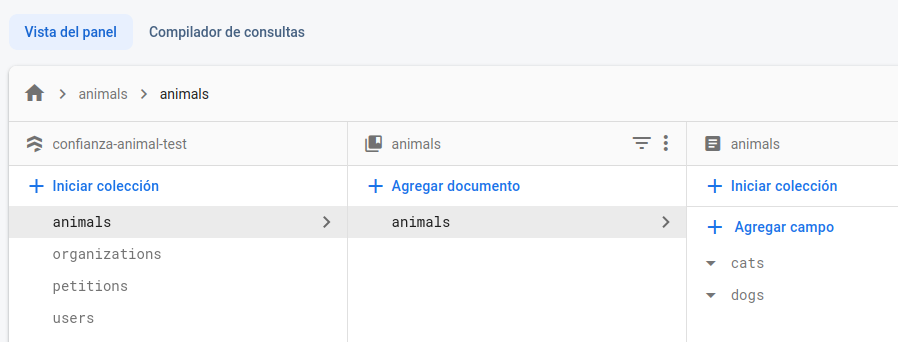
\includegraphics[width=0.9\textwidth]{imgs/database-test.png}
    \caption{Ejemplo de estructura de la base de datos de desarrollo}
    \label{fig:database}
\end{figure}

\newpage

\subsubsection{Datos}\label{subsubsec:datos}

Firebase cuenta con una gran variedad de tipos de datos que se pueden utilizar para almacenar información en la base de datos.
A parte de los tipos de datos básicos como texto, número o booleano, Firebase cuenta con tipos de datos más complejos como
imágenes y archivos que se han utilizado para almacenar las imágenes de los animales, usuarios y organizaciones,
datos de geolocalización en tiempo real o fechas y horas. \\

En este proyecto se han utilizado todo tipo de datos para almacenar la información de los animales, usuarios y organizaciones.
Por ejemplo, para almacenar la información de un animal se ha utilizado el siguiente formato:

\begin{table}[H]
\begin{tabular}{ll}
\textit{\textbf{Variable}} & \textit{\textbf{Tipo de dato}} \\
Nombre                     & \textit{string}                \\
Años                       & \textit{int}                   \\
Meses                      & \textit{int}                   \\
Género                     & \textit{string}                \\
Fotos                      & \textit{photo{[}{]}}             \\
Peso                       & \textit{float}                 \\
Tamaño                     & \textit{string}                \\
Provincia                  & \textit{string}                \\
Castrado                   & \textit{booleano}              \\
Sano                       & \textit{booleano}              \\
Vacunado                   & \textit{booleano}              \\
Fecha de nacimiento        & \textit{datetime}              \\
Microchip                  & \textit{booleano}              \\
Actividad                  & \textit{string}                \\
Urgente                    & \textit{booleano}              \\
Raza                       & \textit{string}                \\
Descripción                & \textit{string}
\end{tabular}
\end{table}

\newpage

\subsubsection{Reglas}\label{subsubsec:reglas}

El sistema de reglas de \textbf{Firebase} son una parte fundamental para la seguridad de la base de datos. Estas reglas
permiten limitar el acceso a la base de datos a usuarios que cumplan una serie de condiciones y se basan en el
lenguaje de expresiones de \textbf{Firebase} (\textit{Firebase's expression language}) que se configuran en
el archivo \textit{firestore.rules} que se encuentra en la raíz del proyecto. \\

Existen dos tipos de reglas: las reglas de validación y las reglas de seguridad. La primera de ellas se encarga de
validar los datos que se van a almacenar en la base de datos y la segunda se encarga de limitar el acceso a la base de datos.
En nuestro caso, como las validaciones se realizan en el \textit{backend} de la aplicación, las reglas de validación
se han dejado vacías y las reglas de seguridad se han configurado en función del entorno de la aplicación. \\

Para la base de datos de desarrollo se quiere que cualquier usuario pueda acceder a la misma, por lo que las reglas
de seguridad permiten el acceso de lectura y escritura a cualquier usuario autenticado:

\begin{lstlisting}
{
    "rules": {
    ".read": "request.auth != null",
    ".write": "request.auth != null"
    }
}
\end{lstlisting}

Para la base de datos de producción las reglas son más estrictas para proteger la información de los usuarios.
De esta forma, solo se permite el acceso a usuarios autenticados y se limita el acceso a la base de datos
en función del tipo de usuario que se haya autenticado y de la colección a la que quiera acceder. Por ejemplo, un usuario normal
puede escribir y leer en su colección de usuario pero no puede escribir en la colección de organizaciones.:

\newpage

\begin{lstlisting}
{
"rules": {
        "Animals": {
            ".read": "request.auth != null",
            ".write": "request.auth != null"
        },
        "Users": {
            "$uid": {
                ".read": "request.auth != null",
                ".write": "request.auth != null && request.auth.uid == $uid"
            }
        },
        "Organization": {
            "$uid": {
                ".read": "request.auth != null",
                ".write": "request.auth != null && request.auth.uid == $uid"
            }
        },
        "Petitions": {
            ".read": "request.auth != null",
            ".write": "request.auth != null"
        }
    }
}

\end{lstlisting}



\subsection{Sprints 5-8}\label{subsec:sprints-5-8}

Una vez que se han completado las tareas que permiten el desarrollo e implementación de la página web y la API, durante los
cuatro siguientes \textit{sprints} se han llevado a cabo las tareas que han permitido la implementación de la página web y la API
así como la realización de los tests y despliegues de ambas:

\begin{itemize}
    \item Creación de \textit{endpoints} para la API.
    \item Creación de componentes para la página web.
    \item Creación de servicios para la página web.
    \item Creación de \textit{tests} para la API y la página web.
\end{itemize}

\subsubsection{Endpoints}\label{subsubsec:endpoints}

Una vez que se ha definido la estructura de la API y conocemos las diferentes clases que se van a utilizar, podemos
pasar a definir e implementar los diferentes \textit{endpoints} para cumplir con los requisitos de la API.\\

Un \textit{endpoint} es un punto de entrada de la API que permite realizar una acción concreta. Es decir,
se refiere a la ruta que se va a utilizar para acceder a un recurso concreto. Por ejemplo, si queremos acceder a la
información de un usuario concreto, la ruta que se utilizaría sería \textit{/users/{user\_id}} siendo \textit{use\_id}
el identificador del usuario. A continuación se van a mostrar los diferentes \textit{endpoints} que se han definido para
el proyecto: \\

\textbf{Ruta:} \textit{/auth}

\begin{itemize}
    \item \textbf{/reset-password}: \textit{POST} \\
    Permite reestablecer la contraseña de un usuario u organización por medio de un correo electrónico que se envía
    a la dirección de correo electrónico registrada en el sistema.
\end{itemize}

\textbf{Ruta:} \textit{/organizations}

\begin{itemize}
    \item \textbf{/me}: \textit{GET} \\
    Permite obtener toda la información de la organización que ha iniciado sesión en el sistema (correo, nombre, foto, etc.).
    \item \textbf{/dogs}: \textit{GET} \\
    Permite obtener todos los perros de la organización que ha iniciado sesión en el sistema en forma de lista.
    \item \textbf{/cats}: \textit{GET} \\
    Permite obtener todos los gatos de la organización que ha iniciado sesión en el sistema en forma de lista.
    \item \textbf{/}: \textit{GET} \\
    Permite obtener una información reducida de todas las organizaciones registradas en el sistema: nombre, correo, foto y provincia.
    \item \textbf{/{organization\_name}}: \textit{GET} \\
    Dado un nombre de organización existente en el sistema, permite obtener toda la información de la organización: nombre, correo, foto, provincia, etc.
    \item \textbf{/dog}: \textit{POST} \\
    Permite crear un nuevo perro en la organización que ha iniciado sesión en el sistema pasando como parámetros los atributos del perro.
    \item \textbf{/cat}: \textit{POST} \\
    Permite crear un nuevo gato en la organización que ha iniciado sesión en el sistema pasando como parámetros los atributos del gato.
    \item \textbf{/register}: \textit{POST} \\
    Permite registrar una nueva organización en el sistema pasando como parámetros los atributos de la organización: nombre, correo, contraseña, teléfono y provincia.
    \item \textbf{/login}: \textit{POST} \\
    Permite iniciar sesión en el sistema pasando como parámetros el correo y la contraseña de la organización.
    \item \textbf{/upload/photo}: \textit{POST} \\
    Permite subir una foto de perfil para la organización que ha iniciado sesión en el sistema.
    \item \textbf{/enable}: \textit{POST} \\
    Permite activar la cuenta de la organización que ha iniciado sesión en el sistema siempre y cuando haya sido desactivada previamente.
    \item \textbf{/dog/{dog\_id}}: \textit{PUT} \\
    Permite modificar los atributos de un perro de la organización que ha iniciado sesión en el sistema pasando como parámetros los atributos del perro.
    \item \textbf{/cat/{cat\_id}}: \textit{PUT} \\
    Permite modificar los atributos de un gato de la organización que ha iniciado sesión en el sistema pasando como parámetros los atributos del gato.
    \item \textbf{/update}: \textit{PUT} \\
    Permite modificar los atributos de la organización que ha iniciado sesión en el sistema pasando como parámetros los atributos a actualizar: teléfono y provincia.
    \item \textbf{/disable}: \textit{DELETE} \\
    Permite desactivar la cuenta de la organización que ha iniciado sesión en el sistema. Una vez desactivada, la organización no podrá iniciar sesión en el sistema.
\end{itemize}

\textbf{Ruta:} \textit{/users}

\begin{itemize}
    \item \textbf{/me}: \textit{GET} \\
    Permite obtener toda la información del usuario que ha iniciado sesión en el sistema (correo, nombre, foto, etc.).
    \item \textbf{/favorites}: \textit{GET} \\
    Permite obtener todos los perros y gatos favoritos del usuario que ha iniciado sesión en el sistema en forma de lista.
    \item \textbf{/favorites/{animal\_id}}: \textit{GET} \\
    Dado un identificador de perro o gato, devuelve si el animal es favorito del usuario que ha iniciado sesión en el sistema.
    \item \textbf{/{user\_id}}: \textit{GET} \\
    Dado un identificador de usuario, permite obtener toda la información del usuario: nombre, correo, foto, etc.
    \item \textbf{/favorites/{animal\_id}}: \textit{POST} \\
    Permite añadir un perro o gato a la lista de favoritos del usuario que ha iniciado sesión en el sistema.
    \item \textbf{/update}: \textit{PUT} \\
    Permite modificar los atributos del usuario que ha iniciado sesión en el sistema pasando como parámetros los atributos a actualizar: nombre, teléfono, provincia...
    \item \textbf{/documentation/{petition\_id}}: \textit{POST} \\
    Permite al usuario simular el envío de documentación a la organización dado un identificador de petición de adopción.
    \item \textbf{/register}: \textit{POST} \\
    Permite registrar un nuevo usuario en el sistema pasando como parámetros los atributos del usuario: correo, nombre y contraseña.
    \item \textbf{/login}: \textit{POST} \\
    Permite iniciar sesión en el sistema pasando como parámetros el correo y la contraseña del usuario.
    \item \textbf{/enable}: \textit{POST} \\
    Permite activar la cuenta del usuario que ha iniciado sesión en el sistema siempre y cuando haya sido desactivada previamente.
    \item \textbf{/upload/photo}: \textit{POST} \\
    Permite subir una foto de perfil para el usuario que ha iniciado sesión en el sistema.
    \item \textbf{/update-documentation/{petition\_id}}: \textit{POST} \\
    Permite al usuario simular la actualización de la documentación de una petición de adopción dado un identificador de petición de adopción
    siempre y cuando la misma haya sido rechazada por la organización previamente.
    \item \textbf{/disable}: \textit{DELETE} \\
    Permite desactivar la cuenta del usuario que ha iniciado sesión en el sistema. Una vez desactivada, el usuario no podrá iniciar sesión en el sistema.
    \item \textbf{/favorites/{animal\_id}}: \textit{DELETE} \\
    Permite eliminar un perro o gato de la lista de favoritos del usuario que ha iniciado sesión en el sistema.
\end{itemize}

\textbf{Ruta:} \textit{/animals}

\begin{itemize}
    \item \textbf{/}: \textit{GET} \\
    Permite obtener todos los perros y gatos registrados en el sistema en forma de lista.
    \item \textbf{/dog/{dog\_id}}: \textit{GET} \\
    Dado un identificador de perro, permite obtener toda la información del perro: nombre, edad, raza, etc.
    \item \textbf{/cat/{cat\_id}}: \textit{GET} \\
    Dado un identificador de gato, permite obtener toda la información del gato: nombre, edad, raza, etc.
    \item \textbf{/dog}: \textit{GET} \\
    Permite obtener todos los perros registrados en el sistema en forma de lista por medio de filtros que se pueden combinar entre sí:
        \begin{itemize}
            \item \textbf{\textit{province}}: Permite filtrar los perros por provincia.
            \item \textbf{\textit{size}}: Permite filtrar los perros por tamaño: mini, pequeño, mediano, grande o gigante.
            \item \textbf{\textit{raze}}: Permite filtrar los perros por raza.
            \item \textbf{\textit{years}}: Permite filtrar los perros por edad numérica.
            \item \textbf{\textit{greater\_or\_equal}}: Booleano que permite filtrar los perros por edad numérica mayor o igual que la especificada en el filtro anterior (\textit{years}).
            \item \textbf{\textit{gender}}: Permite filtrar los perros por género: macho o hembra.
            \item \textbf{\textit{activity}}: Permite filtrar los perros por nivel de actividad: bajo, medio o alto.
            \item \textbf{\textit{is\_urgent}}: Booleano que permite filtrar los perros en caso de ser su adopción urgente o no.
        \end{itemize}
    \item \textbf{/cat}: \textit{GET} \\
    Permite obtener todos los gatos registrados en el sistema en forma de lista por medio de los mismo filtros mencionados anteriormente para el caso de los perros.
    \item \textbf{/dog/{dog\_id}/photos}: \textit{POST} \\
    Permite subir una o varias fotos para un perro dado su identificador.
    \item \textbf{/cat/{cat\_id}/photos}: \textit{POST} \\
    Permite subir una o varias fotos para un gato dado su identificador.
    \item \textbf{/dog/{dog\_id}}: \textit{DELETE} \\
    Permite eliminar un perro del sistema dado su identificador. Sólo válido para organizaciones que además tengan ese animal en su lista.
    \item \textbf{/cat/{cat\_id}}: \textit{DELETE} \\
    Permite eliminar un gato del sistema dado su identificador. Sólo válido para organizaciones que además tengan ese animal en su lista.
    \item \textbf{/dog/{dog\_id}/photo}: \textit{DELETE} \\
    Permite eliminar una foto de un perro dado su identificador y el identificador de la foto.
    \item \textbf{/cat/{cat\_id}/photo}: \textit{DELETE} \\
    Permite eliminar una foto de un gato dado su identificador y el identificador de la foto.
\end{itemize}


\textbf{Ruta:} \textit{/petitions}

\begin{itemize}
    \item \textbf{/user}: \textit{GET} \\
    Permite obtener todas las peticiones de adopción realizadas por el usuario que ha iniciado sesión en el sistema.
    \item \textbf{/{petition\_id}/user}: \textit{GET} \\
    Permite obtener la información de una petición de adopción dado su identificador al usuario que ha iniciado sesión en el sistema.
    \item \textbf{/user/visibles}: \textit{GET} \\
    Permite obtener todas las peticiones de adopción visibles realizadas por el usuario que ha iniciado sesión en el sistema.
    \item \textbf{/user/invisibles}: \textit{GET} \\
    Permite obtener todas las peticiones de adopción invisibles realizadas por el usuario que ha iniciado sesión en el sistema.
    \item \textbf{/organization}: \textit{GET} \\
    Permite obtener todas las peticiones de adopción realizadas a la organización que ha iniciado sesión en el sistema.
    \item \textbf{/dog/{dog\_id}}: \textit{POST} \\
    Permite realizar una petición de adopción para un perro dado su identificador.
    \item \textbf{/cat/{cat\_id}}: \textit{POST} \\
    Permite realizar una petición de adopción para un gato dado su identificador.
    \item \textbf{/{petition\_id}/user}: \textit{POST} \\
    Permite cambiar la visibilidad de una petición de adopción dado su identificador al usuario que ha iniciado sesión en el sistema (visible o invisible).
    \item \textbf{/organization/{petition\_id}}: \textit{POST} \\
    Permite cambiar el estado de una petición de adopción dado su identificador a la organización que ha iniciado sesión en el sistema. El flujo de estados
    se puede ver en la figura~\ref{fig:flujo-peticion}.
    \item \textbf{/{petition\_id}/organization/documentation}: \textit{POST} \\
    Permite actualizar el estado de la petición una vez que el usuario ha subido la documentación requerida para la adopción por parte de la organización.
    \item \textbf{/{petition\_id}/organization/accept-information}: \textit{POST} \\
    Permite actualizar el estado de la petición para indicar que la organización ha aceptado la información aportada por el usuario para una petición de adopción concreta.
    \item \textbf{/{petition\_id}/organization/reject-information}: \textit{POST} \\
    Permite actualizar el estado de la petición para indicar que la organización ha rechazado la información aportada por el usuario para una petición de adopción concreta.
    \item \textbf{/{petition\_id}/organization}: \textit{POST} \\
    Permite actualizar el estado de la petición para indicar que la organización ha aceptado la petición de adopción por parte del usuario.
    \item \textbf{/{petition\_id}/user}: \textit{DELETE} \\
    Permite actualizar el estado de la petición a rechazada por parte del usuario.
    \item \textbf{/{petition\_id}/organization}: \textit{DELETE} \\
    Permite actualizar el estado de la petición a rechazada por parte de la organización.
\end{itemize}

\newpage

\textbf{Ruta:} \textit{/filters}

\begin{itemize}
    \item \textbf{/provinces}: \textit{GET} \\
    Permite obtener todas las provincias que se encuentran en el sistema (Madrid, Barcelona, etc.)
    \item \textbf{/gender}: \textit{GET} \\
    Permite obtener todos los géneros que se encuentran en el sistema (macho, hembra).
    \item \textbf{/activity}: \textit{GET} \\
    Permite obtener todas las actividades que se encuentran en el sistema (baja, media, alta).
    \item \textbf{/size}: \textit{GET} \\
    Permite obtener todos los tamaños que se encuentran en el sistema (pequeño, mediano, grande, etc.)
    \item \textbf{/cat-raze}: \textit{GET} \\
    Permite obtener todas las razas de gatos que se encuentran en el sistema (siamés, persa, etc.)
    \item \textbf{/dog-raze}: \textit{GET} \\
    Permite obtener todas las razas de perros que se encuentran en el sistema (pastor alemán, labrador, etc.)
    \item \textbf{/all}: \textit{GET} \\
    Permite obtener todos los filtros que se encuentran en el sistema (todos los anteriores).
\end{itemize}

\newpage

\subsubsection{Componentes}\label{subsubsec:componentes}

Si ponemos el ejemplo y pensamos que una aplicación web es una casa, los componentes serían las diferentes habitaciones de la casa. Cada componente
se encarga de una tarea concreta y se puede reutilizar en diferentes partes de la aplicación. A su vez, están formados por un fichero \textit{.ts}
que contiene la lógica del componente, un fichero \textit{.html} que contiene la parte visual del componente, un fichero \textit{.scss}
que contiene los estilos del componente y un fichero \textit{.spec.ts} que contiene los tests del componente. \\

Para diferenciar los componentes, en Angular son clases TypeScript decoradas con el decorador \textit{@Component}. Este decorador
es el que define los metadatos del componente como el selector, la plantilla, los estilos, etc. Un ejemplo de componente sería el siguiente:

\begin{lstlisting}
import { Component, OnInit } from '@angular/core';

@Component({
  selector: 'app-home',
  templateUrl: './home.component.html',
  styleUrls: ['./home.component.scss']
})

export class HomeComponent implements OnInit {

  constructor() { }

  ngOnInit(): void {
  }

}
\end{lstlisting}

En este ejemplo se puede observar que el componente se define con el decorador \textit{@Component} y que se le pasan los metadatos
correspondientes. En este caso, el selector del componente es \textit{app-home} y la plantilla y los estilos se encuentran en los ficheros
\textit{home.component.html} y \textit{home.component.scss} respectivamente. \\

Para utilizar un componente en otro, solo es necesario importarlo en la plantilla del componente que se desee. Por ejemplo, si se quiere
utilizar el componente \textit{home} en el componente \textit{app.component}, solo es necesario importarlo en la plantilla del componente
\textit{app.component} de la siguiente forma:

\begin{lstlisting}
<app-home></app-home>
\end{lstlisting}

En el proyecto de la página web se han utilizado los siguientes componentes:

\begin{itemize}
    \item \textbf{app.component}: este componente es el componente principal de la aplicación. Este componente se carga al iniciar la aplicación
    y contiene la llamada al resto de componentes.
    \item \textbf{home.component}: este componente es el componente que se carga al iniciar la aplicación. Este componente contiene la página principal
    de la aplicación.
    \item \textbf{login.component}: este componente contiene la página de inicio de sesión de la aplicación.
    \item \textbf{register.component}: este componente contiene la página de registro de la aplicación.
    \item \textbf{profile.component}: este componente contiene la página de perfil de la aplicación.
    \item \textbf{restore-password.component}: este componente contiene la página de recuperación de contraseña de la aplicación.
    \item \textbf{animals.component}: este componente contiene la página de animales de la aplicación.
    \item \textbf{cat-profile.component}: este componente contiene la página de perfil de un gato de la aplicación.
    \item \textbf{dog-profile.component}: este componente contiene la página de perfil de un perro de la aplicación.
    \item \textbf{cat-view.component}: este componente contiene la página de visualización de un gato de la aplicación.
    \item \textbf{dog-view.component}: este componente contiene la página de visualización de un perro de la aplicación.
    \item \textbf{new-animal.component}: este componente contiene la página de creación de un animal de la aplicación.
\end{itemize}

\newpage

\subsubsection{Servicios}\label{subsubsec:servicios}

Los servicios son clases que se utilizan para organizar y compartir métodos y datos entre diferentes componentes de la aplicación. Estos servicios
se pueden inyectar en los componentes que se deseen y suelen utilizarse para realizar peticiones HTTP a la API.
Para crear un servicio, en Angular se utiliza el decorador \textit{@Injectable}. Este decorador
es el que define los metadatos del servicio como el nombre del servicio, los servicios que se van a inyectar en el servicio, etc. Un ejemplo de servicio
sería el siguiente:

\begin{lstlisting}
import { Injectable } from '@angular/core';

@Injectable({
  providedIn: 'root'
})

export class AuthService {

  constructor() { }
}
\end{lstlisting}

En este ejemplo se puede observar que el servicio se define con el decorador \textit{@Injectable} y que se le pasan los metadatos
correspondientes. En este caso, el servicio se inyecta en el \textit{root} de la aplicación. Los servicios que se han utilizado en el proyecto
de la página web son los siguientes:

\begin{itemize}
    \item \textbf{auth.service}: este servicio se utiliza para realizar las peticiones HTTP relacionadas con la autenticación de la aplicación (inicio de sesión, registro, etc.)
    \item \textbf{user.service}: este servicio se utiliza para realizar las peticiones HTTP relacionadas con los usuarios (organizaciones) de la aplicación.
    \item \textbf{animals.service}: este servicio se utiliza para realizar las peticiones HTTP relacionadas con los animales de la aplicación (crear un animal, obtener todos los animales, etc.)
    \item \textbf{auth.guard}: este servicio se utiliza para comprobar si un usuario está autenticado o no. Este servicio se utiliza para proteger las rutas de la aplicación y
    en caso de que un usuario no esté autenticado, se le redirige a la página de inicio de sesión.
    \item \textbf{filter.service}: este servicio se utiliza para almacenar los filtros que se aplican en la página de animales de la aplicación (raza del animal, tamaño, etc.)
\end{itemize}

\newpage

\subsubsection{Testing}\label{subsubsec:testing}

Con la funcionalidad implementada, se ha procedido a realizar las pruebas necesarias (\textit{tests}) para comprobar que el sistema funciona correctamente.
Esta práctica se considera una de las más importantes a la hora de desarrollar software, ya que permite detectar errores en el sistema de forma
rápida, ayudar a entender cómo funciona el sistema y facilitar el desarrollo del mismo.

Dependiendo de la parte del sistema que se quiera probar, existen diferentes tipos de pruebas como las unitarias, de integración,
de aceptación, rendimiento, etc. En este caso, se han realizado pruebas unitarias para comprobar que las diferentes
partes del sistema funcionan correctamente y pruebas de integración para comprobar que varias partes del sistema funcionan correctamente
cuando se llaman de forma conjunta. \\

También existen diferentes técnicas de desarrollar software en base al desarrollo de pruebas como el \textit{Test Driven Development} (TDD) o
\textit{Behavior Driven Development} (BDD). Estas técnicas consisten en desarrollar las pruebas antes de desarrollar el código, de forma que
se desarrolla el código para que las pruebas pasen. En nuestro caso, no se ha hecho uso de ninguna de estas técnicas debido a la falta de tiempo, pero
se ha realizado un esfuerzo para desarrollar diferentes pruebas que comprueben que el sistema funciona correctamente y que
recojan un gran porcentaje del código escrito (más del 80\%). \\

Todas estas pruebas se pueden realizar de forma manual o de forma automática por medio de herramientas que facilitan el proceso.
En este caso, para la API se ha utilizado la herramienta \href{https://pytest.org/}{pytest} para realizar las pruebas de forma automática y,
gracias a librería \textbf{pytest-cov} se ha obtenido la cobertura de código de las pruebas. Para la aplicación web se ha utilizado el framework
de testing \href{https://jasmine.github.io/}{Jasmine} junto a \textbf{Karma} para automatizar la ejecución de las pruebas.

Para saber en todo momento el porcentaje de código que se está probando
y tener una estadísticas de los \textit{tests}, se ha utilizado la herramienta \textit{pytest-cov} la cual es necesaria
explicar su funcionamiento antes de explicar los diferentes \textit{tests} que se han realizado. \\

\newpage

\textbf{Pytest-cov} es una extensión de \textit{pytest} que se utiliza para comprobar la cobertura de los \textit{tests} de una aplicación.
Para utilizar esta extensión, es necesario instalarla en el entorno virtual de la aplicación y añadir la
siguiente línea al fichero \textit{pytest.ini}:

\begin{lstlisting}
[pytest]
addopts = --cov=app --cov-report=html
\end{lstlisting}

En esta línea se indica que se quiere comprobar la cobertura de los \textit{tests} de la aplicación y que se quiere generar un informe en formato HTML.
En el informe se incluye información sobre la cantidad de líneas de código que se han ejecutado, la cantidad de líneas de código que no se han ejecutado,
la cantidad de líneas de código que se han omitido durante la ejecución de los \textit{tests}. \\

Ahora, ¿por qué esta herramienta es fiable para comprobar la cobertura de los \textit{tests}? Esta herramienta utiliza la
técnica conocida como "instrumentación de código" que consiste en rastrear la ejecución de un programa y comprobar si se ha ejecutado
una línea de código o no por medio un programa interno que se llama \textit{coverage.py}. Un 100\% de cobertura de los \textit{tests} no significa
que el código esté libre de errores, pero sí que es un indicador de que el código está bien probado y que es más probable que no contenga errores.
En el siguiente artículo se explica con más detalle
cómo funciona esta técnica y por qué aumenta la calidad y fiabilidad de los \textit{tests}: \href{https://www.codemag.com/article/1701081/Improve-Code-Quality-Using-Test-Coverage}{Pytest Code Coverage} \\

En las siguientes imágenes se puede observar el informe de cobertura de los \textit{tests} de la API:

\begin{figure}[H]
    \centering
    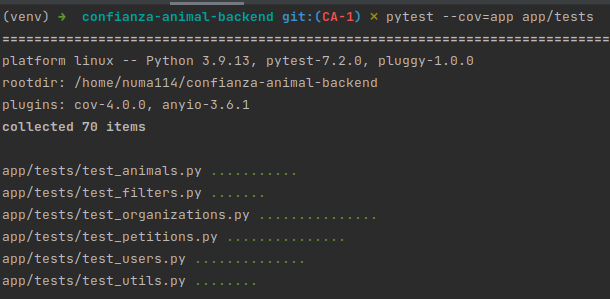
\includegraphics[width=0.8\textwidth]{imgs/coverage2-big.png}
    \caption{Informe de cobertura de los tests de la API}
    \label{fig:coverage2}
\end{figure}

\begin{figure}[H]
    \centering
    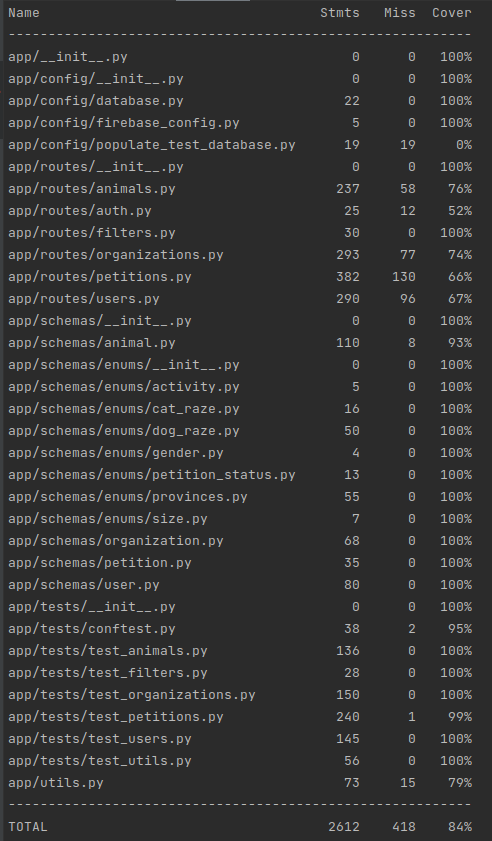
\includegraphics[width=0.8\textwidth]{imgs/coverage1.png}
    \caption{Informe de cobertura de los tests de la API}
    \label{fig:coverage1}
\end{figure}

\newpage

Como se puede observar en las imágenes, la \textbf{cobertura} de los \textit{tests} de la API es del 84\%, la cual se ha obtenido
a partir de la ejecución de 70 \textit{tests} diferentes a lo largo de los diferentes ficheros que se van a explicar
a continuación y que abordan las diferentes casuísticas que se puedan dar en el \textit{endpoint} así como en la base de datos
incluyendo los errores que se puedan producir: \\

\textbf{test\_animals.py}: este fichero contiene los \textit{tests} relacionados con los endpoints de la ruta \textit{/animals} de la API:

\begin{itemize}
    \item \textbf{test\_get\_all\_animals}: este \textit{test} comprueba que se obtienen todos los animales de la base de datos correctamente
    \item \textbf{test\_get\_dog\_by\_id}: este \textit{test} comprueba que se obtiene un perro dado su identificador correctamente.
    \item \textbf{test\_get\_cat\_by\_id}: este \textit{test} comprueba que se obtiene un gato dado su identificador correctamente.
    \item \textbf{test\_get\_dog\_by\_filters}: este \textit{test} comprueba que se obtienen todos los perros que cumplen con los filtros
    especificados por el usuario correctamente (raza, tamaño, etc.) y las diferentes casuísticas que se pueden dar.
    \item \textbf{test\_get\_cat\_by\_filters}: este \textit{test} comprueba que se obtienen todos los gatos que cumplen con los filtros
    especificados por el usuario correctamente (raza, tamaño, etc.) y las diferentes casuísticas que se pueden dar.
    \item \textbf{test\_upload\_dog\_photos}: este \textit{test} comprueba que se suben las fotos de un perro correctamente.
    \item \textbf{test\_upload\_cat\_photos}: este \textit{test} comprueba que se suben las fotos de un gato correctamente.
    \item \textbf{test\_delete\_dog\_photo}: este \textit{test} comprueba que se borra una foto de un perro correctamente.
    \item \textbf{test\_delete\_cat\_photo}: este \textit{test} comprueba que se borra una foto de un gato correctamente.
    \item \textbf{test\_delete\_dog\_by\_id}: este \textit{test} comprueba que se borra un perro dado su identificador correctamente.
    \item \textbf{test\_delete\_cat\_by\_id}: este \textit{test} comprueba que se borra un gato dado su identificador correctamente.
\end{itemize}

\textbf{test\_filters.py}: este fichero contiene los \textit{tests} relacionados con los endpoints de la ruta \textit{/filters} de la API:

\begin{itemize}
    \item \textbf{test\_get\_provinces}: este \textit{test} comprueba que se obtienen todas las provincias correctamente.
    \item \textbf{test\_get\_gender}: este \textit{test} comprueba que se obtienen todos los géneros de los animales correctamente.
    \item \textbf{test\_get\_activity}: este \textit{test} comprueba que se obtienen todas los niveles de actividad de los animales correctamente.
    \item \textbf{test\_get\_size}: este \textit{test} comprueba que se obtienen todos los tamaños de los animales correctamente.
    \item \textbf{test\_get\_cat\_raze}: este \textit{test} comprueba que se obtienen todas las razas de los gatos correctamente.
    \item \textbf{test\_get\_dog\_raze}: este \textit{test} comprueba que se obtienen todas las razas de los perros correctamente.
    \item \textbf{test\_get\_all}: este \textit{test} comprueba que se obtienen todos los filtros anteriores correctamente.
\end{itemize}

\textbf{test\_users.py}: este fichero contiene los \textit{tests} relacionados con los endpoints de la ruta \textit{/users} de la API:

\begin{itemize}
    \item \textbf{test\_user\_register}: este \textit{test} comprueba que se registra un usuario correctamente.
    \item \textbf{test\_login\_user}: este \textit{test} comprueba que se loguea un usuario correctamente.
    \item \textbf{test\_get\_user\_profile}: este \textit{test} comprueba que se obtiene el perfil de un usuario correctamente.
    \item \textbf{test\_user\_favorites}: este \textit{test} comprueba que se obtienen los animales favoritos de un usuario correctamente.
    \item \textbf{test\_check\_if\_animals\_is\_in\_favorites}: este \textit{test} comprueba que se comprueba si un animal está en favoritos de un usuario correctamente.
    \item \textbf{test\_get\_user\_by\_id}: este \textit{test} comprueba que se obtiene un usuario dado su identificador correctamente.
    \item \textbf{test\_envy\_user\_documentation}: este \textit{test} comprueba que se envía la documentación de un usuario correctamente.
    \item \textbf{test\_post\_user\_favorites}: este \textit{test} comprueba que se añade un animal a favoritos de un usuario correctamente.
    \item \textbf{test\_enable\_user}: este \textit{test} comprueba que se habilita un usuario correctamente.
    \item \textbf{test\_disable\_user}: este \textit{test} comprueba que se deshabilita un usuario correctamente.
    \item \textbf{test\_upload\_profile\_photo}: este \textit{test} comprueba que se sube la foto de perfil de un usuario correctamente.
    \item \textbf{test\_update\_user}: este \textit{test} comprueba que se actualiza un usuario correctamente.
    \item \textbf{test\_update\_user\_documentation}: este \textit{test} comprueba que se actualiza la documentación de un usuario correctamente.
    \item \textbf{test\_delete\_favorite}: este \textit{test} comprueba que se borra un animal de favoritos de un usuario correctamente.
\end{itemize}

\textbf{test\_organizations.py}: este fichero contiene los \textit{tests} relacionados con los endpoints de la ruta \textit{/organizations} de la API:

\begin{itemize}
    \item \textbf{test\_organization\_register}: este \textit{test} comprueba que se registra una organización correctamente.
    \item \textbf{test\_login\_organization}: este \textit{test} comprueba que se loguea una organización correctamente.
    \item \textbf{test\_post\_cat}: este \textit{test} comprueba que se añade un gato correctamente a una organización.
    \item \textbf{test\_post\_dog}: este \textit{test} comprueba que se añade un perro correctamente a una organización.
    \item \textbf{test\_get\_organization\_profile}: este \textit{test} comprueba que se obtiene el perfil de una organización correctamente.
    \item \textbf{test\_get\_dogs\_from\_organization}: este \textit{test} comprueba que se obtienen todos los perros de una organización correctamente.
    \item \textbf{test\_get\_cats\_from\_organization}: este \textit{test} comprueba que se obtienen todos los gatos de una organización correctamente.
    \item \textbf{test\_get\_organizations}: este \textit{test} comprueba que se obtienen todas las organizaciones correctamente.
    \item \textbf{test\_get\_organization\_by\_name}: este \textit{test} comprueba que se obtiene una organización dado su nombre correctamente.
    \item \textbf{test\_upload\_profile\_photo\_organization}: este \textit{test} comprueba que se sube la foto de perfil de una organización correctamente.
    \item \textbf{test\_modify\_cat}: este \textit{test} comprueba que se actualizan los datos de un gato correctamente.
    \item \textbf{test\_modify\_dog}: este \textit{test} comprueba que se actualizan los datos de un perro correctamente.
    \item \textbf{test\_enable\_organization}: este \textit{test} comprueba que se habilita una organización correctamente.
    \item \textbf{test\_disable\_organization}: este \textit{test} comprueba que se deshabilita una organización correctamente.
    \item \textbf{test\_update\_organization}: este \textit{test} comprueba que se actualizan los datos de una organización correctamente.
\end{itemize}

\textbf{test\_petitions.py}: este fichero contiene los \textit{tests} relacionados con los endpoints de la ruta \textit{/petitions} de la API:

\begin{itemize}
    \item \textbf{test\_ask\_for\_dog}: este \textit{test} comprueba que la solicitud de un perro se realiza correctamente.
    \item \textbf{test\_ask\_for\_cat}: este \textit{test} comprueba que la solicitud de un gato se realiza correctamente.
    \item \textbf{test\_get\_petitions\_by\_user}: este \textit{test} comprueba que se obtienen todas las solicitudes de un usuario correctamente.
    \item \textbf{test\_get\_petition\_by\_id\_user}: este \textit{test} comprueba que se obtiene una solicitud dado su identificador y el identificador de un usuario correctamente.
    \item \textbf{test\_get\_petitions\_by\_organization}: este \textit{test} comprueba que se obtienen todas las solicitudes de una organización correctamente.
    \item \textbf{test\_reject\_petition\_by\_user}: este \textit{test} comprueba que se rechaza una solicitud por parte de un usuario correctamente.
    \item \textbf{test\_reject\_petition\_by\_organization}: este \textit{test} comprueba que se rechaza una solicitud por parte de una organización correctamente.
    \item \textbf{test\_accept\_petition\_by\_organization}: este \textit{test} comprueba que se acepta una solicitud por parte de una organización correctamente.
    \item \textbf{test\_change\_petition\_visibility\_by\_user}: este \textit{test} comprueba que se cambia la visibilidad de una solicitud por parte de un usuario correctamente.
    \item \textbf{test\_get\_petitions\_visibles\_by\_user}: este \textit{test} comprueba que se obtienen todas las solicitudes visibles de un usuario correctamente.
    \item \textbf{test\_get\_petitions\_invisibles\_by\_user}: este \textit{test} comprueba que se obtienen todas las solicitudes invisibles (archivadas) de un usuario correctamente.
    \item \textbf{test\_update\_state\_petition\_by\_organization}: este \textit{test} comprueba que se actualiza el estado de una solicitud por parte de una organización correctamente.
    \item \textbf{test\_reject\_documentation\_by\_organization}: este \textit{test} comprueba que se rechaza la documentación enviada por un usuario en una solicitud por parte de una organización correctamente.
    \item \textbf{test\_reject\_information\_by\_organization}: este \textit{test} comprueba que se rechaza la información enviada por un usuario en una solicitud por parte de una organización correctamente.
    \item \textbf{test\_accept\_information\_by\_organization}: este \textit{test} comprueba que se acepta la información enviada por un usuario en una solicitud por parte de una organización correctamente.
\end{itemize}

\textbf{test\_utils.py}: este fichero contiene los \textit{tests} relacionados con las funciones auxiliares de la API:

\begin{itemize}
    \item \textbf{test\_exists\_email\_in\_organization}: este \textit{test} comprueba si existe un email en una organización o no.
    \item \textbf{test\_exists\_phone\_in\_organization}: este \textit{test} comprueba si existe un teléfono en una organización o no.
    \item \textbf{test\_exists\_name\_in\_organization}: este \textit{test} comprueba si existe un nombre como nombre de una organización o no.
    \item \textbf{test\_exists\_id\_in\_user}: este \textit{test} comprueba si existe un identificador en un usuario o no.
    \item \textbf{test\_exists\_dog\_in\_animals}: este \textit{test} comprueba si existe un perro en la lista de animales de una organización o no.
    \item \textbf{test\_exists\_cat\_in\_animals}: este \textit{test} comprueba si existe un gato en la lista de animales de una organización o no.
    \item \textbf{test\_get\_dog\_or\_cat\_by\_filters}: este \textit{test} comprueba que se obtienen los perros o gatos que cumplen los filtros correctamente.
    \item \textbf{test\_generate\_uuid}: este \textit{test} comprueba que se genera un identificador único correctamente.
\end{itemize}

A parte de todos los \textit{tests} mencionados anteriormente, se han realizado una serie de \textit{fixtures} (datos de prueba) para poder realizar los \textit{tests} de forma correcta.
Estas \textit{fixtures} se encuentran en el fichero \textbf{conftest.py} y son para poder acceder a los \textit{endpoints} que requieren
de autenticación, por tanto existe una \textit{fixture} para la autenticación de un usuario y otra para la autenticación de una organización.
Se identifican por medio de los \textit{decorators} \@pytest.fixture y se usan directamente en los \textit{tests} que las requieren pasándolas como parámetro. \\

Un ejemplo de \textbf{test de integración} sería el \textit{test\_accept\_petition\_by\_organization} ya que
para poder realizarlo se necesita comprobar toda la funcionalidad asociada a la aceptación de una solicitud por parte de una organización:

\begin{enumerate}
    \item Se crea una organización y un usuario.
    \item Se crea una solicitud por parte del usuario a la organización.
    \item La organización actualiza el estado de la solicitud a \textit{Información pendiente de revisión}.
    \item La organización comprueba que la información aportada es correcta, acepta la información enviada por el usuario y actualiza el estado de la solicitud a \textit{Pendiente de documentación}.
    \item El usuario envía la documentación requerida por la organización.
    \item La organización acepta la documentación enviada por el usuario y actualiza el estado de la solicitud a \textit{Aceptada}.
\end{enumerate}

Es por ello que para realizar este \textit{test} es necesario completar todo el flujo de la petición (ver completo en la figura:~\ref{fig:flujo_peticion}) y comprobar que
la funcionalidad asociada a cada paso se realiza correctamente teniendo en cuenta también los posibles casos que se pueden
dar durante el proceso, como por ejemplo que la organización rechace la información enviada por el usuario y actualice el estado de la solicitud a \textit{Información rechazada}
y que el usuario envíe de nuevo la información requerida por la organización. \\

En cuanto a los tests de la aplicación web, por cada componente y servicio existe un fichero de \textit{tests} asociado bajo
la extensión \textbf{.spec.ts}. Dado que el proyecto está enfocado en el desarrollo de la API, no se han realizado demasiados
\textit{tests} en la aplicación web, pero se han realizado algunos para comprobar que los componentes y servicios funcionan correctamente. \\

Un ejemplo de \textit{test} muy básico de un componente en el que se comprueba que se crea correctamente sería el siguiente:

\begin{lstlisting}
  describe('DogViewComponent', () => {
      let component: DogViewComponent;
      let fixture: ComponentFixture<DogViewComponent>;

      beforeEach(async () => {
        await TestBed.configureTestingModule({
          imports: [
            DogViewComponent,
            HttpClientTestingModule,
            ToastrModule.forRoot(),
            StoreModule.forRoot({}),
          ],
        }).compileComponents();

        fixture = TestBed.createComponent(DogViewComponent);
        component = fixture.componentInstance;
        fixture.detectChanges();
      });

      it('should create', () => {
        expect(component).toBeTruthy();
      });
  });
\end{lstlisting}



\subsection{Sprints 9-11}\label{subsec:sprints-9-11}

En los tres últimos \textit{sprints} se han llevado a cabo las tareas que han permitido el cierre del proyecto. En concreto, se ha
llevado a cabo la finalización de los \textit{tests} pendientes, el cierre final de tareas y la finalización
y revisión de la página web, del funcionamiento de la API y de la documentación del proyecto.

\subsubsection{Documentación de la API}\label{subsubsec:documentacion-api}

La documentación de la API se ha realizado utilizando \href{https://www.swagger.io/}{Swagger}. Swagger es una herramienta que permite
documentar APIs de forma sencilla y que proporciona una interfaz gráfica para poder probar las APIs. Esta documentación
se encuentra de forma pública en el siguiente enlace: \href{https://confianza-animal-backend.onrender.com/docs}{Confianza Animal Docs}. \\

Todos los endpoints en la documentación cuentan con un ejemplo de petición: (ver en siguiente página)

\begin{figure}[H]
    \centering
    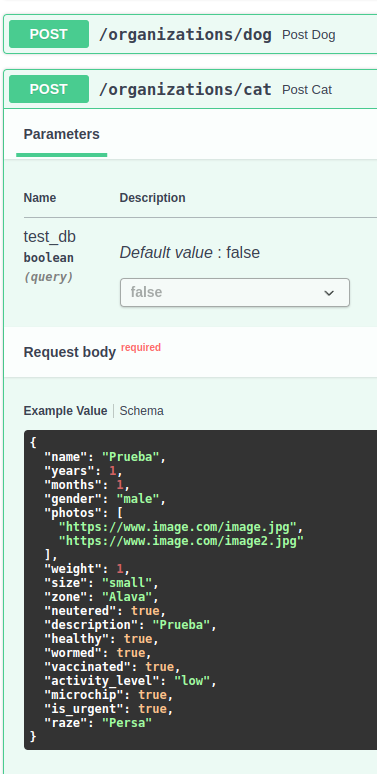
\includegraphics[width=0.5\textwidth]{imgs/swagger1.png}
    \caption{Ejemplo de petición en la documentación}
    \label{fig:endpoint-example}
\end{figure}

\newpage

Y un ejemplo de respuesta y de error: \\

\begin{figure}[H]
    \centering
    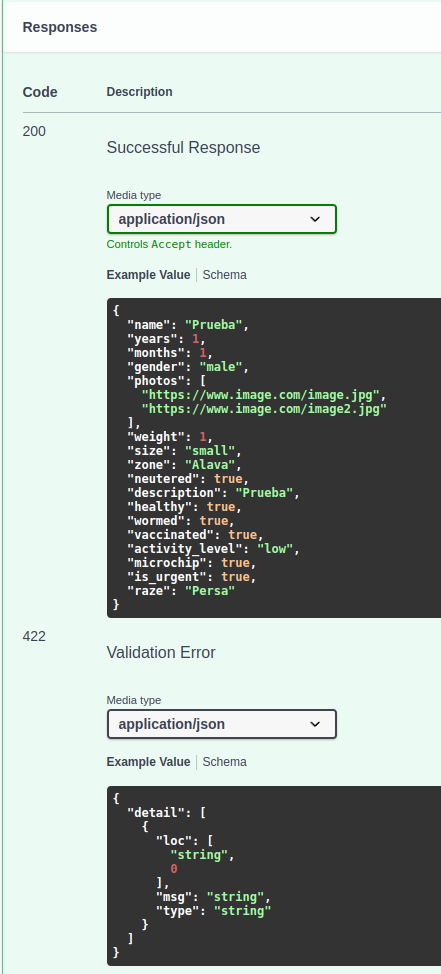
\includegraphics[width=0.5\textwidth]{imgs/swagger2.png}
    \caption{Ejemplo de respuesta y error en la documentación}
    \label{fig:endpoint-example-2}
\end{figure}

De esta forma, ayuda a los desarrolladores a entender cómo funciona la API y a realizar peticiones de forma correcta sin
necesidad de tener que leer el código. También permite a usuarios con menos conocimientos técnicos tener la oportunidad
de utilizar la API ya que la interfaz es muy intuitiva.


\section{Despliegue de la página web}\label{sec:despliegue-de-la-pagina-web}

Para el despliegue de la página web se ha utilizado \textit{Firebase Hosting}, un servicio de hosting web que permite
desplegar aplicaciones web estáticas de forma sencilla y rápida. \textit{Firebase Hosting} ofrece un plan gratuito que
incluye 10 GB de almacenamiento y 10 GB de transferencia de datos al mes, más que suficiente para el desarrollo de este
proyecto en fase de pruebas. \\

Tal y como se mencionó en la sección:~\ref{sec:eleccion-de-herramientas-y-tecnologias}, gracias a que la página web
está desarrollada con \textbf{Angular} y esta ser un framework de \textbf{Google}, la integración con \textit{Firebase}
es muy sencilla y no presenta problemas de compatibilidad a la hora de llevar a cabo el despliegue para el cual
se han seguido los siguientes pasos:

\begin{enumerate}
    \item Instalar \textit{Firebase CLI} por medio de \textit{npm} con el comando \textit{npm install -g firebase-tools}.
    \item Iniciar sesión en \textit{Firebase} con el comando \textit{firebase login}.
    \item Inicializar el proyecto con el comando \textit{firebase init}.
    \item Seleccionar la opción \textit{Hosting} y el proyecto de \textit{Firebase} que se quiere desplegar.
    \item Seleccionar la carpeta que contiene el código de la página web.
    \item Ejecutar el comando \textit{firebase deploy} para desplegar la página web.
\end{enumerate}

Es por ello que de esta forma, cada vez que se realice un cambio en el código de la página web se puede desplegar de forma automática
con el comando \textit{firebase deploy}. Otra ventaja que ofrece esta herramienta es que permite la creación de un dominio personalizado
para la página web y la configuración de certificados \textit{TSL} gratuitos para que la página web se pueda acceder por medio de
\textit{HTTPS} con el dominio personalizado. De forma predeterminada, \textit{Firebase Hosting} ofrece un dominio gratuito
con el siguiente formato: \textit{<nombre-proyecto>.web.app} que se accede por medio de \textit{HTTPS}. En este caso, la ruta
de acceso a la página web es: \url{https://confianza-animal.web.app}.

En la siguiente figura se puede ver el resultado de acceder al enlace de la página web: \\

\begin{figure}[H]
    \centering
    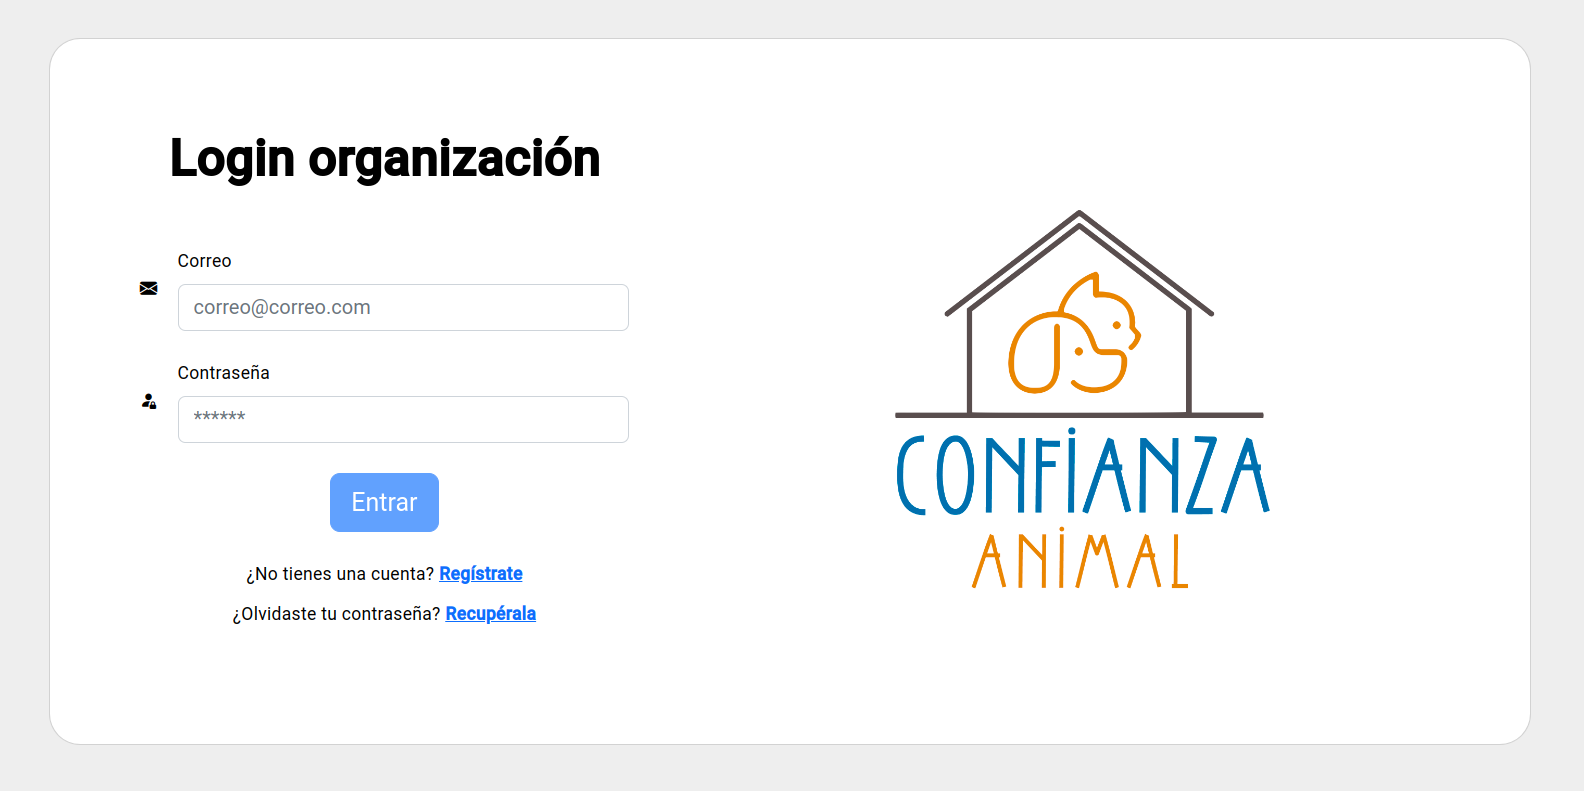
\includegraphics[width=0.9\textwidth]{imgs/despliegue-web.png}
    \caption{Despliegue de la página web en Firebase Hosting}
    \label{fig:firebase-hosting}
\end{figure}

\section{Despliegue de la API}\label{sec:despliegue-de-la-api}

Para el despliegue de la API y su documentación se ha utilizado \textbf{Render}, un servicio de hosting con certificados \textit{TSL}
gratuitos, una \textit{CDN} global, protección \textit{DDoS}, redes privadas y despliegues automáticos desde \textit{GitHub}.
Los detalles de seguridad del proyecto así como los protocolos que se utilizan para la comunicación entre el cliente y el servidor
se pueden consultar en profundidad en la sección de seguridad:~\ref{sec:seguridad}. \\

El motivo principal por el que se ha escogido Render para el despliegue de la API es por su facilidad de uso y por su
integración con \textit{GitHub}. Render permite desplegar la API de forma automática cada vez que se realiza un cambio
en el repositorio de \textit{GitHub} y permite la creación de un dominio personalizado para la API. \\

Otro tema que ha decidido la elección de esta herramienta ha sido el precio. Render ofrece un plan gratuito que incluye
750 horas de uso, 100 GB de ancho de banda y 500 minutos de \textit{build} que se renuevan cada mes. Este plan ha sido
más que suficiente para el desarrollo del proyecto pero en caso de que el proyecto se siguiera desarrollando, Render
ofrece planes de pago que permiten escalar los recursos de forma sencilla y sin necesidad de preocuparse por la
gestión de los servidores. \\

\begin{figure}[H]
    \centering
    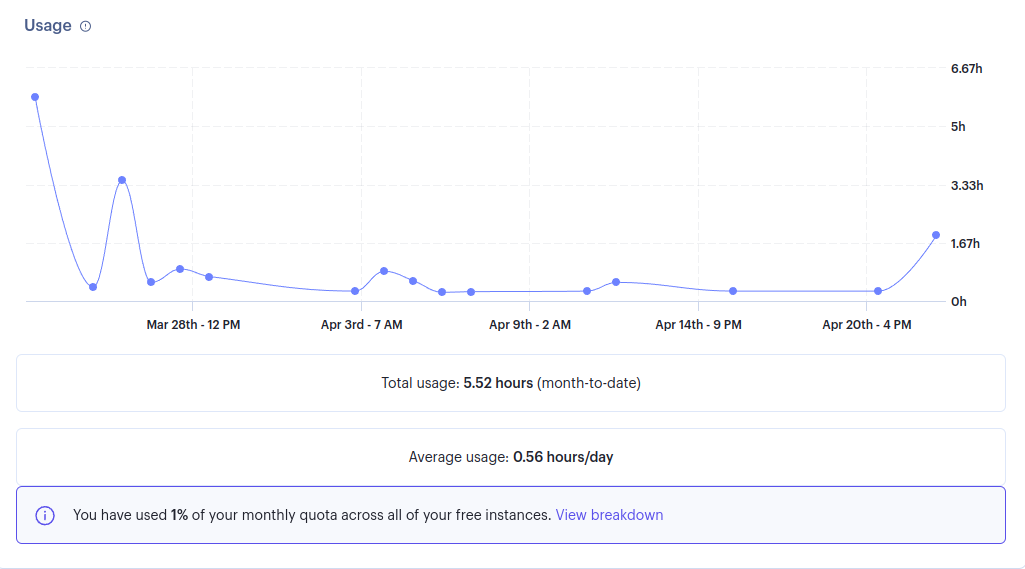
\includegraphics[width=0.9\textwidth]{imgs/usage.png}
    \caption{Uso total de la API}
    \label{fig:usage-render}
\end{figure}

\begin{figure}[H]
    \centering
    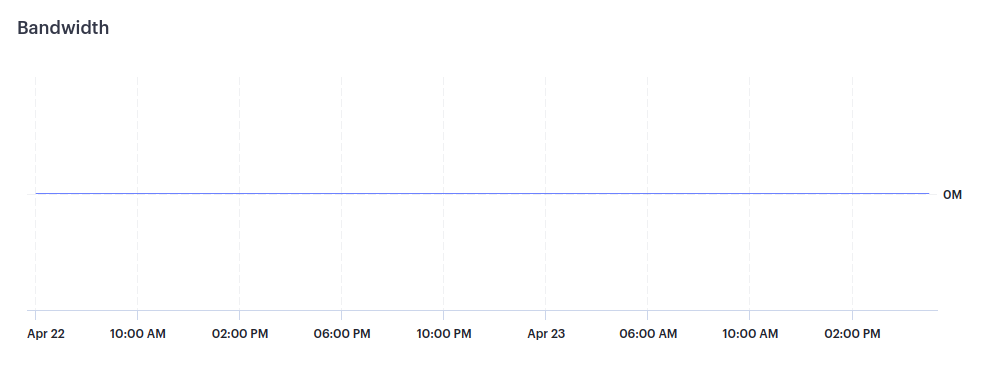
\includegraphics[width=0.9\textwidth]{imgs/bandwidth.png}
    \caption{Ancho de banda total de la API}
    \label{fig:bandwidth-render}
\end{figure}

Los pasos que se han seguido para realizar el despliegue han sido los siguientes:

\begin{enumerate}
    \item Vincular la cuenta de \textit{GitHub} con Render.
    \item Crear un nuevo servicio que se conecte a nuestro repositorio deseado.
    \item Crear un \textit{environment} (entorno) para el servicio. En este caso se han añadido las variables de entorno
    correspondientes a la base de datos y a los servicios de Firebase y tres ficheros que almacenan claves privadas:
    un json con las claves de la base de datos de producción, un json con las claves de la base de datos de test
    y el fichero \textit{.env} con todas las variables de entorno que se utilizan en el proyecto.
    \item Instalar los paquetes necesarios para el despliegue de la API. En este caso al ser un proyecto con \textit{Python}
    se ha utilizado el fichero \textit{requirements.txt} el cual por medio del comando \textit{pip install -r requirements.txt}
    se incluyen paquetes como \textit{pytest}, \textit{firebase}, \textit{FastAPI}, \textit{uvicorn}, etc.
    \item Para lanzar la API se utiliza el comando \textit{uvicorn main:app --host 0.0.0.0 --port 10000} que permite
    correr el servidor de \textit{FastAPI} en el puerto 10000 (puerto por defecto de Render).
    \item Se selecciona la rama de nuestro repositorio se quiere desplegar (\textit{main} en este caso) y la rama de
    despliegue automático cada vez que se realice un \textit{push} (cambio en el código).
\end{enumerate}

Un aspecto importante a tener en cuenta es que para el despliegue de la API se lanza el comando \textit{pytest} para
ejecutar todos los tests antes de hacer el despliegue. Esto permite asegurarnos de que nuestro código funciona correctamente
y que la funcionalidad cumple los \textit{tests} realizados en el proyecto antes de sacar una nueva versión de forma pública.

\begin{figure}[H]
    \centering
    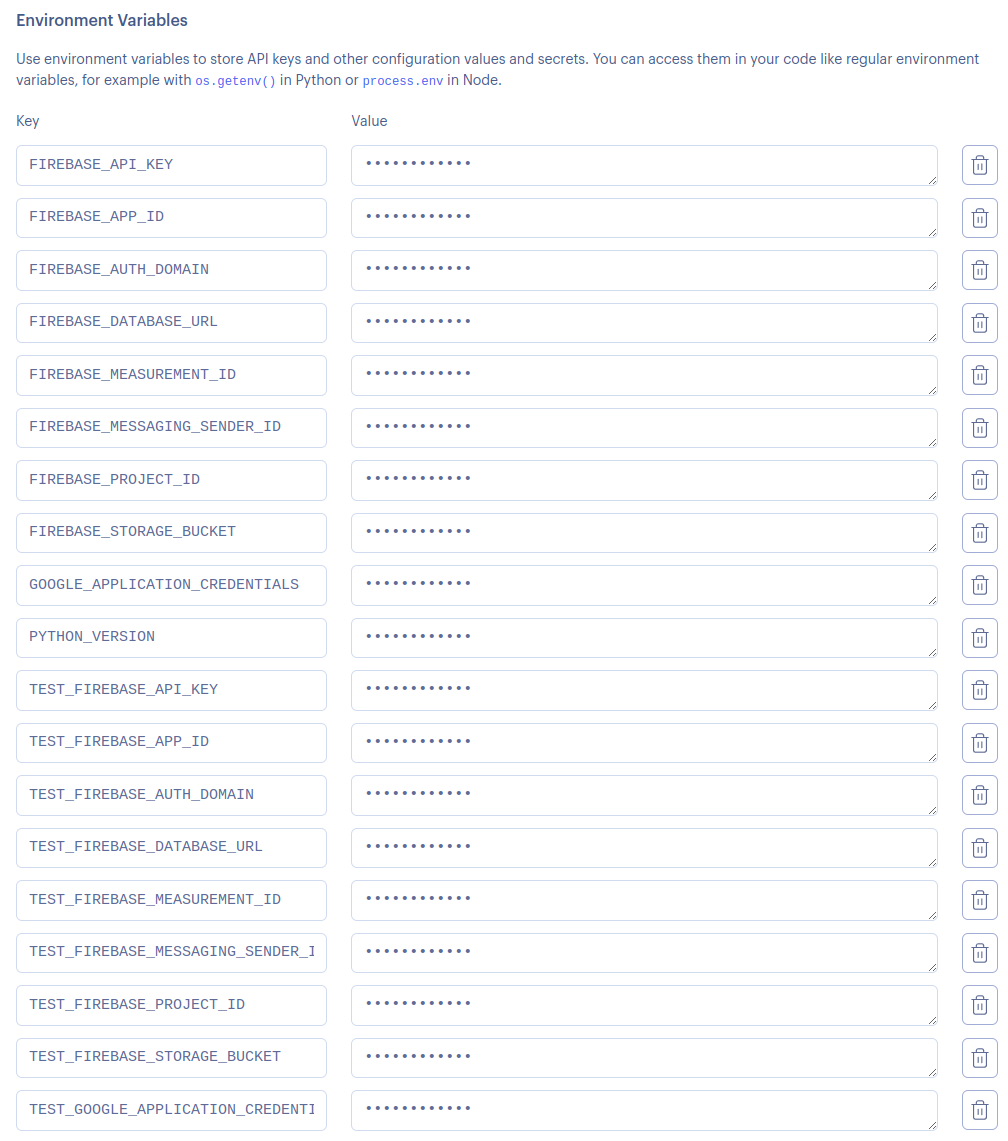
\includegraphics[width=0.8\textwidth]{imgs/env-variables.png}
    \caption{Variables de entorno}
    \label{fig:environment-variables}
\end{figure}

\begin{figure}[H]
    \centering
    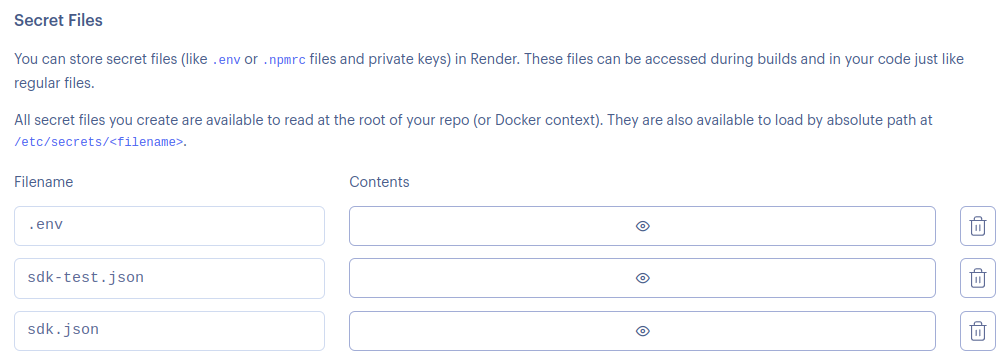
\includegraphics[width=0.8\textwidth]{imgs/secret-files.png}
    \caption{Ficheros secretos}
    \label{fig:secret-files}
\end{figure}

\newpage

    \chapter{Seguridad y ética}\label{ch:seguridad-y-etica}

La adopción de animales es un proceso que requiere de una gran responsabilidad por parte de los adoptantes. Por ello,
la seguridad de los datos es un tema importante a tener en cuenta en este proyecto para asegurar que los usuarios
se sientan cómodos y seguros a la hora de utilizar la aplicación. Para conseguirlo, se han tomado una serie de medidas
que se explicarán en este capítulo como la encriptación de datos, el registro de usuarios por medio de doble
factor de autenticación, la gestión de la información y los términos y condiciones de uso. \\

La ética también es otra consideración importante en el proyecto ya que es importante evitar que se fomente
la compra de animales, la cría irresponsable, el abandono de mascotas y la explotación animal. Las organizaciones
y asociaciones que se dedican a la adopción de animales tienen como objetivo principal el bienestar de los animales
y la concienciación de la sociedad. Por ello, es importante que la aplicación no se utilice para fines distintos
a los que se ha diseñado y que se cumplan los términos y condiciones de uso establecidos (ver sección~\ref{subsec:terminos-y-condiciones}).

\section{Seguridad}\label{sec:seguridad}

Como se ha mencionado, la \textbf{seguridad} de los datos en un proyecto de este tipo es crucial para que los usuarios no
comprometan su información personal. Por ello, se han tomado una serie de medidas para garantizar la seguridad
de los mismos tanto en la \textbf{API} como en la página web y en la base de datos.

\subsection{API}\label{subsec:api}

Para el desarrollo seguro de la API se han seguido las recomendaciones de seguridad de la documentación de \textit{FastAPI}
y se han implementado las siguientes medidas:

\begin{itemize}
    \item \textbf{Encriptación de datos}: se ha utilizado la librería \textit{pycryptodome} para encriptar las contraseñas de los
    usuarios y evitar que se puedan ver en texto plano. Para ello, se ha utilizado el algoritmo \textit{AES} (Advanced Encryption Standard) con una clave
    de 32 bytes y un vector de inicialización de 16 bytes. La clave y el vector de inicialización se han generado
    aleatoriamente y se han guardado en el fichero \textit{.env} para que no se puedan ver en el código fuente. Este algoritmo
    consiste en una serie de rondas de sustitución y permutación de bits que se repiten 10, 12 o 14 veces dependiendo
    del tamaño de la clave. El tamaño de la clave se mide en bits y puede ser de 128, 192 o 256 bits. Cuanto mayor sea
    el tamaño de la clave, más segura será la encriptación. En este caso, se ha utilizado una clave de 256 bits que
    es la más segura de las tres. Fuente:~\cite{aes}
        \begin{figure}[H]
            \centering
            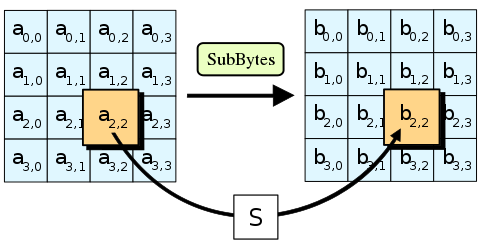
\includegraphics[width=0.8\textwidth]{imgs/aes.png}
            \caption{Encriptación de datos con AES. Fuente de imagen: \href{https://es.wikipedia.org/wiki/Advanced_Encryption_Standard}{Wikipedia}}
            \label{fig:encriptacion}
        \end{figure}
    \item \textbf{Autenticación y autorización}: se ha utilizado el protocolo estándar \textit{OAuth2} para la autenticación y autorización de usuarios.
    Este estándar permite que los usuarios autoricen a una aplicación a acceder a sus datos en otro servicio sin tener
    que compartir sus credenciales. Para ello, se ha utilizado la librería \textit{OAuth2} de \textit{FastAPI} que permite
    generar tokens de acceso y tokens de actualización. Los tokens de acceso se utilizan para acceder a los recursos
    protegidos y los tokens de actualización se utilizan para obtener nuevos tokens de acceso cuando estos han expirado.
    \item \textbf{Validaciones de datos}: se han utilizado las validaciones de datos de \textit{FastAPI} para asegurar que los datos
    que se envían a la \textbf{API} son correctos. Para ello, se han utilizado los tipos de datos de \textit{Pydantic} que permiten
    definir los tipos de datos de cada campo y las validaciones que deben cumplir. Por ejemplo, se ha definido que
    los números de teléfono deben tener el prefijo de España (+34) seguido de 9 dígitos y que los correos electrónicos deben tener el formato
    correcto. Además, se han definido los campos que son obligatorios y los que son opcionales para cada \textit{endpoint}.
    \item \textbf{Auditoría}: por medio de \textbf{Render} se ha podido monitorizar el uso de la \textbf{API} y comprobar que los usuarios
    no hacen un uso indebido de la misma. Se puede controlar el número de peticiones que se hacen a cada \textit{endpoint},
    la forma en la que se hacen las peticiones y el tiempo de respuesta de cada una de ellas. Además, se puede controlar
    el número de usuarios que se registran en la aplicación y el número de usuarios que se autentican en la misma.
    \item \textbf{Doble factor de autenticación}: para evitar que los usuarios puedan crear cuentas con datos falsos, se ha
    implementado un sistema de doble factor de autenticación. Gracias a los servicios de \textit{Firebase}, cada vez que
    un usuario u organización se registra en la aplicación, se le envía un correo electrónico con un enlace para verificar
    su cuenta. De esta forma, se evita que se puedan crear cuentas con datos falsos y se asegura que los usuarios
    que se registran en la aplicación son reales. Cuando se quiere restaurar la contraseña ocurre lo mismo, se envía
    un correo electrónico con un enlace para que el usuario pueda cambiar su contraseña.
    \item \textbf{Sistema seguro de contraseñas}: para evitar que las contraseñas de los usuarios sean vulnerables, se ha
    impuesto una serie de restricciones a la hora de crear una contraseña. Las contraseñas deben tener una longitud mínima
    de 8 caracteres y deben contener al menos una letra mayúscula, una letra minúscula, un número y un carácter especial
    \item \textbf{Vulnerabilidad en endpoints}: para evitar que un ataque de fuerza bruta pueda vulnerar la seguridad de la \textbf{API},
    los códigos de respuesta de cada \textit{endpoint} no dan información valiosa sobre el error que se ha producido. Por ejemplo,
    si se quisiera restaurar la contraseña de un usuario y se envía un correo electrónico que no está registrado en la
    aplicación, el código de respuesta sería 200 (OK) en lugar de 404 (Not Found). De esta forma, se evita que un atacante
    pueda saber si un correo electrónico está registrado en la aplicación o no.
\end{itemize}

Toda esta serie de medidas de seguridad permiten que la \textbf{API} sea en la medida de lo posible segura y que los usuarios
puedan hacer uso de ella sin tener que preocuparse por la seguridad de sus datos, lo cual garantiza la permanencia
de los mismos en el tiempo.

\subsection{Página web}\label{subsec:pagina-web}

Para la página web también se han tomado medidas de seguridad para garantizar la seguridad de los datos de las organizaciones.
En este caso, se ha utilizado el protocolo \textit{HTTPS} (Hyper Text Transfer Protocol Secure) que es la versión segura
del protocolo \textbf{\textit{HTTP}}. Este protocolo permite que los datos que se envían entre el servidor y el cliente estén encriptados
y que no puedan ser leídos por terceros. Para ello, se ha utilizado un certificado \textbf{\textit{TSL (Transport Layer Security)}} que
es un protocolo que permite la comunicación segura entre dos entidades. Es un archivo digital que se utiliza para verificar
la identidad de un sitio web o servidor y para encriptar la información que se envía entre el servidor y el cliente.
Cuando un usuario accede a un sitio web que utiliza \textbf{\textit{HTTPS}} (protocolo seguro basado en TLS), el navegador web
autentica el servidor web y luego utiliza la clave pública del servidor para encriptar la información que se envía al
servidor. El servidor web desencripta la información utilizando su clave privada y luego procesa la información. De esta
forma, se garantiza que los datos que se envían entre el servidor y el cliente están encriptados y que no pueden ser
leídos por terceros. \\

También por medio de \textbf{tokens} como \textbf{JWT} (JSON Web Token) se ha podido implementar un sistema de autenticación
y autorización seguro. Cuando un usuario se autentica en la aplicación, se le envía un token de acceso que contiene
información sobre el usuario y que tiene una duración de 15 minutos. Este token se utiliza para acceder a los recursos
protegidos de la aplicación. Cuando el token expira, se utiliza un token de actualización para obtener un nuevo token
de acceso. En la siguiente imagen se describe el proceso de login de un usuario en la aplicación:

\begin{figure}[H]
    \centering
    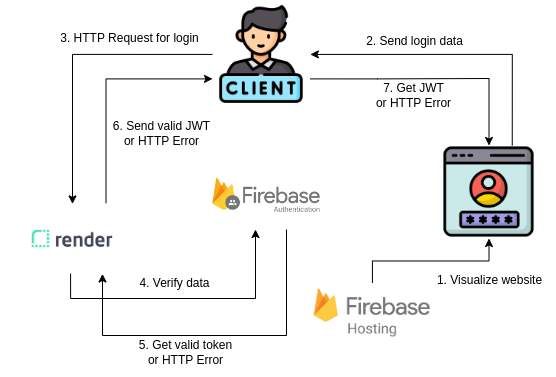
\includegraphics[width=0.8\textwidth]{imgs/login-diagrama.png}
    \caption{Proceso de login de un usuario en la aplicación}
    \label{fig:login}
\end{figure}

Como se puede observar en la imagen, cuando un usuario se autentica en la aplicación, se le envía un token de acceso
que contiene información sobre el usuario o un error en caso de que las credenciales sean incorrectas. Este token
se utiliza para acceder a los recursos protegidos de la aplicación. \\

Otra técnica que se ha utilizado para garantizar la seguridad de los datos de las organizaciones es la \textbf{protección \textit{CSRF}} (Cross-Site Request Forgery).
Esta técnica consiste en añadir un \textit{token} a cada formulario de la aplicación para evitar que un atacante pueda enviar
peticiones a la aplicación en nombre de un usuario. También por medio de los \textbf{encabezados \textit{CORS}} (Cross-Origin Resource Sharing) se ha
podido controlar el acceso a los recursos de la aplicación. Por ejemplo, se ha definido que solo se puede acceder a los
recursos de la aplicación desde la página web y no desde otras aplicaciones.

\newpage

\subsection{Base de datos}\label{subsec:base-de-datos}

La principal seguridad que se ha tomado en la base de datos ha sido la de crear reglas de seguridad de \textit{Firebase} tal
y como se ha explicado en la sección~\ref{subsec:firebase}. Estas reglas de seguridad permiten controlar el acceso a la
lectura y escritura de los datos de la base de datos. \\

\textbf{Firebase} utiliza los protocoles \textit{SSL/TLS} para cifrar las comunicaciones entre la aplicación y la base de datos. De
esta forma no se puede interceptar el tráfico de la aplicación y leer los datos que se envían a la base de datos. También
implementa protección frente a ataques de fuerza bruta, limitando el número de intentos de autenticación que se pueden hacer
en un periodo de tiempo por dirección IP. \\

Otra forma con la que \textbf{Firebase} protege los datos de la base de datos es con técnicas de prevención de inyección
de código malicioso en las consultas a la base de datos. Por ejemplo, si se intenta hacer una consulta a la base de datos
con una clave que no existe, se devuelve un error en lugar de devolver un resultado vacío. De esta forma, se evita que
un atacante pueda saber si una clave existe en la base de datos o no. \\

En resumen, gracias a todas las medidas de seguridad que implementa \textbf{Firebase}, se garantiza la seguridad de los
datos de las organizaciones y usuarios, se evita los posibles ataques contra la base de datos y hace que la aplicación
se convierta en una aplicación segura y fiable para todos los usuarios.

\section{Ética}\label{sec:etica}

Para abordar el tema de la ética en el desarrollo de la aplicación, se ha tenido en cuenta el código ético de la ACM (Association
for Computing Machinery)~\cite{acm-code-of-ethics}. Este código ético se basa en 7 principios generales que se deben tener en cuenta
a la hora de desarrollar un software. A continuación, se explica cómo se han aplicado estos principios en el desarrollo
de la aplicación web y \textbf{API}:

\begin{itemize}
    \item \textbf{Contribuir al bienestar y a la calidad de vida de los usuarios}: La aplicación se ha desarrollado con el
    objetivo de ayudar a las organizaciones a gestionar sus animales y a encontrarles un hogar. De esta forma, se contribuye
    al bienestar de los animales y a la calidad de vida de las personas que los adoptan.
    \item \textbf{Evitar daños a otros}: La aplicación no tiene ningún tipo de contenido que pueda dañar a los usuarios de
    la misma. Además, se han tomado medidas de seguridad para garantizar la seguridad de los datos de las organizaciones y
    de los usuarios.
    \item \textbf{Ser honesto y confiable}: La aplicación es honesta y confiable ya que no se ha ocultado ningún tipo de
    información a los usuarios y se ha desarrollado con el objetivo de ayudar a las organizaciones a gestionar sus animales
    y a encontrarles un hogar.
    \item \textbf{Ser justo y tomar medidas para no discriminar}: La aplicación no discrimina a ningún tipo de usuario
    siempre y cuando se cumplan las condiciones de uso de la misma.
    \item \textbf{Respetar el trabajo necesario para producir nuevas ideas, inventos, trabajos creativos y artefactos informáticos}:
    La aplicación respeta el trabajo necesario para producir nuevas ideas, inventos, trabajos creativos y artefactos informáticos
    ya que no se ha copiado ningún tipo de código de otras aplicaciones y se ha desarrollado desde cero.
    \item \textbf{Respetar la privacidad}: La aplicación respeta la privacidad de los usuarios ya que no se almacena ningún
    tipo de información personal de los usuarios y se ha implementado un sistema de autenticación y autorización seguro.
    \item \textbf{Respetar la confidencialidad}: La aplicación respeta la confidencialidad de los datos de las organizaciones
    y de los usuarios ya que se han tomado medidas de seguridad que se pueden ver en detalle en los apartados anteriores.
\end{itemize}

Para concluir con este apartado es interesante mencionar que a la hora de realizarse un registro en la aplicación web,
se necesitan aprobar los términos y condiciones de uso de la misma. En estos términos y condiciones se explica que la
aplicación no se hace responsable de los datos que se almacenan en la misma y que se pueden eliminar los datos de la
aplicación en cualquier momento. También se explica que la aplicación no se hace responsable de los daños que se puedan
ocasionar por el uso de la misma y que se pueden modificar los términos y condiciones en cualquier momento.

\subsection{Gestión de la información}\label{subsec:gestion-de-la-informacion}

En este apartado se explica cómo se ha gestionado la información de los usuarios y de las organizaciones. \\

En primer lugar, se ha tenido en cuenta la \textbf{Ley Orgánica de Protección de Datos}~\cite{ley-proteccion-datos} (LOPD) que
regula el tratamiento de los datos personales y las obligaciones que deben asumir los responsables de una web o una
aplicación web que almacene datos de carácter personal. \\

En esta ley se establece que los datos de carácter personal deben ser tratados de forma lícita, leal y transparente en
relación con el interesado y recogidos con fines determinados, explícitos y legítimos. También se establece que los datos
de carácter personal deben ser adecuados, pertinentes y limitados a lo necesario en relación con los fines para los que
son tratados. \\

Teniendo en cuenta esta ley y las diferentes medidas de seguridad que se han tomado en la aplicación, se puede afirmar
que se ha gestionado la información de los usuarios y de las organizaciones de forma correcta y que se ha cumplido con
la LOPD en todo momento durante el desarrollo de la aplicación web y \textbf{API}.

\subsection{Términos y condiciones}\label{subsec:terminos-y-condiciones}

Para realizar el registro en la aplicación web, se deben aceptar los términos y condiciones de uso de la misma. En estos
términos y condiciones es importante identificar los siguientes puntos:

\begin{itemize}
    \item \textbf{Responsabilidad}: La aplicación no se hace responsable de los datos que se almacenan en la misma y que
    se pueden eliminar los datos de la aplicación en cualquier momento.
    \item \textbf{Daños}: La aplicación no se hace responsable de los daños que se puedan ocasionar por el uso de la misma.
    \item \textbf{Modificación}: La aplicación se reserva el derecho de modificar los términos y condiciones en cualquier
    momento.
    \item \textbf{Aceptación}: La aceptación de los términos y condiciones es obligatoria para poder registrarse en la
    aplicación web.
    \item \textbf{Uso}: El uso de la aplicación web está limitado a las organizaciones que se dedican a la protección de
    animales y no a cualquier tipo de usuario que quiera registrarse en la aplicación.
    \item \textbf{Datos personales}: La aplicación no almacena ningún tipo de información personal de los usuarios.
    \item \textbf{Actualización y revisión}: La aplicación se reserva el derecho de actualizar y revisar los términos y
    condiciones en cualquier momento.
\end{itemize}

En la siguiente imagen vemos como en el registro se añade un checkbox para aceptar los términos y condiciones de uso de
la aplicación web: \\

\begin{figure}[H]
    \centering
    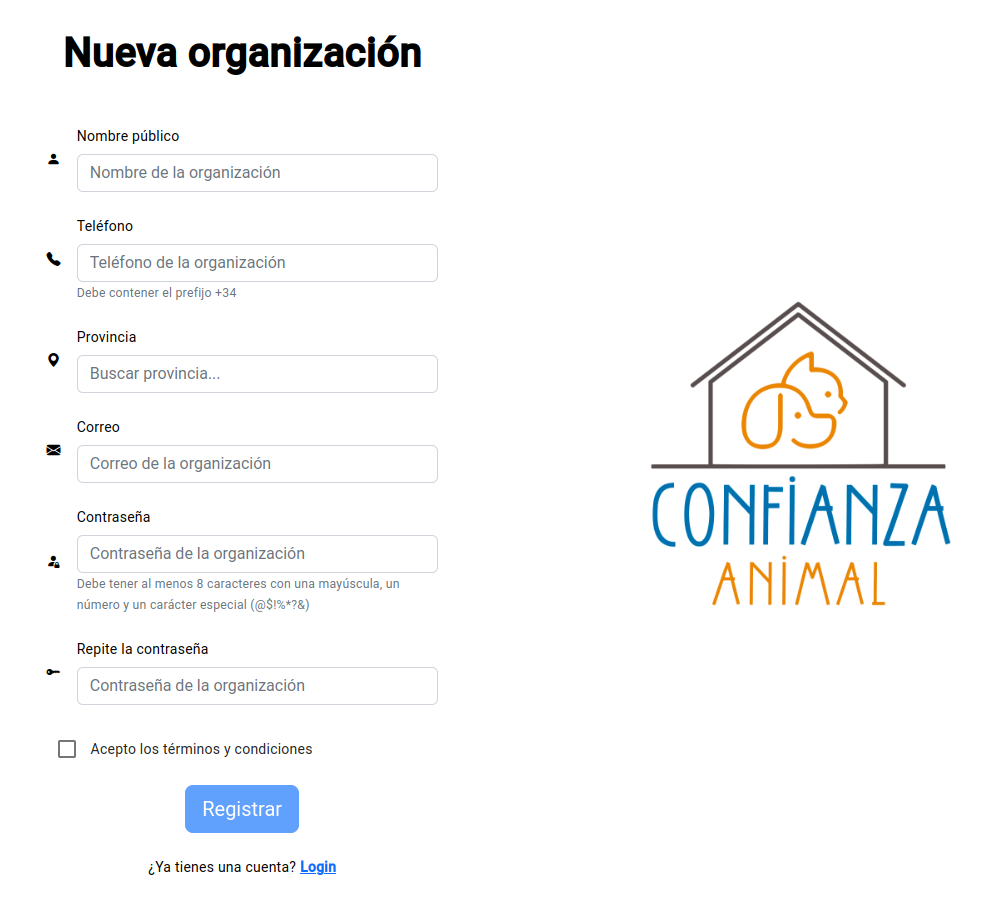
\includegraphics[width=0.9\textwidth]{imgs/registro.png}
    \caption{Registro de organizaciones en aplicación web}
    \label{fig:terminos-y-condiciones}
\end{figure}

    \chapter{Conclusiones y Trabajos Futuros}\label{ch:conclusiones-y-trabajos-futuros}

En este apartado se concluye la documentación y se proponen posibles trabajos futuros que se podrían realizar como
mejoras o ampliaciones del proyecto.

\section{Conclusiones}\label{sec:conclusiones}

Tras varios meses de trabajo, se ha conseguido desarrollar una \textbf{API} que permite la gestión de organizaciones
y sus animales en adopción y de usuarios que pueden adoptarlos. También se ha implementado una aplicación web que
comprueba el funcionamiento de la \textbf{API} y permite a las organizaciones registrar sus datos y animales en adopción
y gestionar las solicitudes de adopción de los mismos. \\

Tanto la página web como la \textbf{API} han sido desplegadas en la nube, concretamente en \textbf{Firebase} y \textbf{Render}
respectivamente. Esto permite que el trabajo realizado pueda ser utilizado por cualquier persona que quiera crear una
aplicación web o móvil que permita la gestión de animales en adopción. \\

No ha sido una tarea sencilla, ya que como en todo proyecto, se han encontrado dificultades que han hecho que el desarrollo
se haya alargado más de lo esperado. A esto se suma la falta de experiencia tanto el desarrollo de \textbf{APIs} como en
el desarrollo de aplicaciones web así como en los \textit{frameworks} que se han utilizado. \\

Para concluir, me gustaría comentar de forma personal que los conocimientos que he
adquirido a lo largo del grado me han ayudado a cumplir los objetivos que me propuse al inicio del proyecto. Además, he
aprendido a utilizar nuevas herramientas, he mejorado mis habilidades de programación y he aprendido a trabajar de forma
autónoma, organizada y responsable. Pero como el tiempo para el desarrollo del proyecto ha sido limitado, en el siguiente
apartado propongo una serie de posibles mejoras y ampliaciones que se podrían realizar en un futuro.


\section{Trabajos Futuros}\label{sec:trabajos-futuros}

Para mejorar y seguir ampliando el proyecto, se proponen las siguientes mejoras:

\begin{itemize}
    \item Permitir a los usuarios la posibilidad de notificar irregularidades en los animales en adopción de forma que se puedan
    denunciar casos de maltrato animal.
    \item Permitir a las organizaciones llevar un registro de vacunaciones y tratamientos de los animales en adopción.
    \item Añadir la posibilidad de realizar donaciones a las organizaciones.
    \item Permitir a los usuarios marcar una organización como favorita.
\end{itemize}

    \newpage
    \bibliography{bibliografia}\addcontentsline{toc}{chapter}{Bibliografía}
    \bibliographystyle{unsrt}
\end{document}
